\documentclass[
  BCOR=10mm, % Binding correction ([default=0])
  DIV=12, % Number of divisions for the page spread construction ([default=9])
  twoside, % two sided ([default='oneside'])
  headsepline, % separate head-line from content optically (horizontal row) (KOMA-Doc, Ch.'Kopf- und Fusszeilen')
  listof=totoc, % include list of tables/figures to list of content
  bibliography=totoc, % include list of literature to list of content
  index=totoc, % include index to list of content
  abstract=true, % Put an coresponding header to the abstract ([default='abstractoff'])
  numbers=noenddot, % suppress ending dot in numberations (required? -> 'pointednumbers')
]{cs-thesis}

\hyphenation{
}

\usepackage{booktabs}
\usepackage{hyperref}
\addbibresource{literature.bib}

%%%%%%%%%%%%%%%%%%%%
%%% THE DOCUMENT %%%
%%%%%%%%%%%%%%%%%%%%

\begin{document}

    %
% intro.tex
%

% start with non paging
% note: authorship itself has another empty
\pagestyle{empty}

% title (includes acknowledgment/dedication)
\maketitle

% authorship
\makeauthorship

% abstract
\makeabstract

% Zusammenfassung auf deutsch
% \cleardoubleemptypage
\makezusammenfassung

% table of contents
\cleardoubleemptypage
\pagenumbering{roman}
\pagestyle{plain}
\tableofcontents
 % Title, abstract, ToC, etc. 
    
    % prepare main document
    \ofoot[\pagemark]{\pagemark} % show page numbering on chapter starts
    \nocite{*} % show all references in bibliography, no matter if used or not
    \cleardoublepage
    \pagenumbering{arabic}
    \pagestyle{chapterstyle}
    
    \acresetall % reset acronym counter
    %
% chapter1.tex
%

\chapter{Introduction}
\label{cha:introduction}
Development in internet infrastructure has led to higher interconnectedness over the course of the last century.
Interacting with companies and governmental facilities is primarily done online.
Deploying servers, providing specific services to the public, has become common place in daily life.
With a continually growing importance of these servers, exploiting them becomes attractive for malicious actors.
Identifying threats and security breaches is required to provide consistent uptime of servers.
While traditional firewalls provide a starting point in defense against exploitation, they are not impenetrable.
Common attacks, such as a \ac{DoS} attack, can circumvent these measures by imitating genuine clients.
Draining system resources by sending illegitimate communication requests is simultaneously easy to do, and hard to protect against.

Additional monitoring of incoming traffic is done by \ac{IDSs}.
Interpreting a clients intent is done by analyzing system logs, as well as system and network resources.
To actually combat incoming attacks, an \ac{IPS} is required which actively defends system resources.
A common industry standard for such an \ac{IPS} is Fail2ban\cite{git:fail2ban}.
It scans a variety of information available on the host system, predominantly using log files as its source, technically making it a \ac{HIPS}.
Clients deemed a threat to the host system are prohibited to interact with the host.
Fail2ban achieves this by modifying the systems firewall.

However, previous work has shown that Fail2ban does not scale well when having to process a large number of log files instantaneously\cite{mikolajczak:ebpf}.
For networks with high bandwidth, a sudden influx in log messages can indicate an ongoing attack on the system.
Fail2ban being unable to efficiently perform its duties in these heavy-load scenarios has serious downfalls.
This inconsistent performance makes the system vulnerable against \ac{DoS} attacks.
It was determined that the intrinsic file-based logging approach of Fail2ban does not provide the necessary bandwidth or low latency required to repel \ac{DoS} attacks successfully.

To remedy this issue a light-weight alternative to Fail2ban was developed: Simplefail2ban\cite{raatschen:ipc}.
While inheriting the basic functionality of Fail2ban, this application provides the option to replace slow file-based logging with alternative \ac{IPC}.
During development, a shared memory \ac{IPC} type was implemented.
This allowed Simplefail2ban to outperform Fail2ban effortlessly\cite{raatschen:ipc}, but if better alternatives exist remains unclear.

The main goal of this thesis is to design and implement an \ac{IPC} mode based on UNIX domain sockets into Simplefail2ban in order to protect against \ac{DoS} attacks.
This includes an easily usable \ac{API} and the option to attach multiple reader processes to the \ac{IPC} architecture.
In order to evaluate the performance of this socket \ac{IPC}, a comparison with the already implemented shared memory and file \ac{IPC} types is conducted.

Firstly, this thesis introduces background information regarding both Fail2ban and Simplefail2ban.
An explanation of the basic concepts used for the \ac{IPC} is also included.
Following that, a chapter is dedicated to introducing the design of the UNIX socket \ac{IPC} architecture.
A separate chapter will explain the intricacies of the implementation of said \ac{IPC} type.
In addition, the design of all experiments will be explained.
To determine the performance of the socket \ac{IPC}, an extensive evaluation of the conducted measurements is included in this thesis.
Finally, a summary of the findings of this thesis and a verdict on performance of both the shared memory and socket \ac{IPC} type for Simplefail2ban is included.
    
    \acresetall % reset acronym counter
    %
% chapter2.tex
%

\chapter{Background \& Motivation}
\label{cha:background}
The following section establishes a definition for Host-based intrusion detection/prevention systems and introduces the example Fail2ban.
An introduction to an alternative solution and its necessity, Simplefail2ban, will also be discussed.
Lastly, any external tools used extensively in this thesis will also be discussed. 

\section{Host-based intrusion detection and prevention}
Intrusion detection and prevention systems are tasked with monitoring the system and ensuring that no threat is present.
The restriction to only utilize data available on the host system, differentiates a host-based intrusion detection system from other forms of IDS (TODO: Abbreviation).
In general, this includes collecting and analyzing data, identifying outliers and responding to any potential threats or unusual behavior to minimize any potential harm.
According to James P. Andersons study "Computer security threat monitoring and surveillance"(TODO: cite this) a threat is any deliberate attempt to either
\begin{itemize}
    \itemsep0em
    \item access data.
    \item manipulate data.
    \item or render a system unreliable or unusable.
\end{itemize}

With the ever present risk of a system having a previously unknown vulnerability, proactive measures must be taken to prevent malicious actors exploits.
Real-time intrusion detection systems are required to achieve this goal.
The motivation for such a system is outlined by Dorothy E. Denning (TODO: cite this):
\begin{itemize}
    \itemsep0em
    \item The majority of systems have vulnerabilities, rendering them susceptible. 
    \item Replacing systems with known vulnerabilities is difficult. Specific features may only be present in the less-secure system.
    \item Developing absolutely secure systems is difficult, since the explicit absence of vulnerabilities can rarely be proven.
    \item Secure systems remain vulnerable to insiders misusing their privileges.
\end{itemize}

For the purposes of this paper, defending against a Denial of Service, the assumption that any system is exploitable will suffice.
\noindent

Host-based intrusion detection systems generally collect data from multiple sources, freely provided by the host.
Such auditing of data needs to be tamper-proof and nonbypassable.
Low-level system calls, often containing such data, are preferred.
The anomaly based approach allows an intrusion detection system to create profiles representing legitimate behavior of clients, users and applications.
Any deviation is interpreted as an attack on the system.
This retains the advantage of not explicitly defining attack patterns, creating a more robust system which can identify new threats on its own.\cite{HIDPS}

\subsection{Fail2ban}
Fail2ban is an open-source intrusion prevention system developed in Python and runs at the user space level.
In contrast to a intrusion detection system, an IPS such as Fail2ban takes deliberate measures once a threat has been identified to stop attacks on a system early.
By default, Fail2ban scans a variety of commonly used log files using regular expressions (regex), also called filters, to identify threats.
It is therefore able to parse and monitor log data of a variety of different applications.
A client will be identified as a threat if it repeatedly fails a certain task, for example establishing a TCP connection.
Such a client is then banned by modifying the system firewall to deny any incoming traffic from banned IP addresses. TODO: Cite https://github.com/fail2ban/fail2ban/wiki/How-fail2ban-works

In detail, Fail2ban creates so called jails.
These jails are saved on persistent storage.
Therefore, restarting Fail2ban or the machine running it will not result in a loss of current jail entries.
A jail consists of a log path, a certain filter, an action and a variety of customizable parameters.
The filter requires at least one regex pattern.
These patterns define what behavior Fail2ban should tolerate or not.
An action, commonly a command or program, is to be executed once a client has been deemed a threat.
Further parameters define the time the action will be active (ban time) and how often bad behavior of a client must be identified (ban limit) in log files to issue a ban.
In practice, if a client fails to adhere to what the filter of a jail defines as proper behavior, vital information of that client would be deduced by the analyzed log messages.
This includes to IP address of the client.
A ban will then be issued and a certain action, for example dropping all traffic with the source IP of the banned client, would be performed.
To issue such a ban, temporary changes to the Linux firewall, using iptables, are performed.
iptables allows user space programs, such as Fail2ban, to modify, add and remove rules for packet filtering.
An incoming package has to pass each set of rules before reaching the destined application.
Fail2ban creates a separate rule for each banned client via iptables.
New incoming packets are checked against all rules defined by iptables, or until they infringe at least one rule.
Especially when many clients need to be banned, this is a clear deficit.
Each banned client corresponds to one additional rule future traffic has to be compared to.\cite{mikolajczak:ebpf}.

\subsection{Extended Berkeley Packet Filter}
The extended Berkeley Packet Filter (eBPF) provides to opportunity to run user-generated code in a privileged setting, such as the kernel.
Such eBPF programs are written in high-level programming languages, for example C.
Compilers convert these programs to eBPF bytecode in user space.
Successfully deploying the code requires an eBPF verifier to accept the program.
This is done exclusively in kernel space to not risk the security of the operating system.
If the eBPF program is accepted, the program will be converted to eBPF native code.
There are several hooks to which an eBPF program can be attached to.
Depending on the chosen hook, the eBPF program is deployed in or even before the network stack.
Meaning, the eBPF program receives incoming traffic while the operating system is still processing it in kernel space.\cite{mikolajczak:ebpf}

In this thesis, the XDP Driver hook is used for all eBPF programs.
Simply put, the eBPF program and its user-generated code is run before the kernel has performed its usual processing steps for incoming traffic.
Here, the program will receive each incoming packet and can decide to let it pass to the kernel unhindered, or drop it.

Since eBPF programs are event-driven, they only handle one packet at a time.
In order to communicate with other programs or even store information, eBPF Maps are used.
These maps are a key-vale store and provide persistent storage.
However, the size of eBPF maps can not be changed during runtime and needs to be defined before creating them.\cite{mikolajczak:ebpf}

This provides a significant advantage over the iptables approach of filtering packets.
With eBPF programs it is possible to drop unwanted packets before they reach the computation heavy kernel network stack.
And while eBPF programs have a variety of useful applications, for this thesis they are only used to either accept packets and pass them to the kernel or drop them to lighten the load.

\subsection{Simplefail2ban}
During research conducted by Florian Mikolajczak, it has been proven that Fail2ban performs poorly when dealing with large amounts of incoming unwanted traffic.
This issue remained even after an alternative, and competitive, method of filtering incoming traffic using eBPF programs was implemented.
To remedy this shortcoming, Simplefail2ban was developed by Paul Raatschen.
It was suspected that Fail2ban was loosing performance by exclusively utilizing traditional file-based logging.
The goal was to implement an IPS that can prohibit malicious actors from sending traffic to the host system, similarly to Fail2ban, without having to rely on file-based logging.

Simplefail2ban provides the option to use a shared memory section to receive log messages.
This proved to be a faster method to transmit log messages from an application directly to Simplefail2ban.
And whilst the method of acquisition of the log messages has changed drastically, the general requirements of banning a client has not changed compared to Fail2ban.
The IPS still monitors incoming log messages for disallowed behavior. \footnote{Since Simplefail2ban is just a prototype, the distinction between allowed and disallowed behavior is based upon the payload of incoming traffic.}
Each violation of the rules imposed by Simplefail2ban results in the clients IP being logged in a hashtable.
If the number of entries for one IP address is over the defined ban limit, that client is banned via one of the banning threads of Simplefail2ban.
This ban is facilitated by adding the IP address to a list of banned clients with the current timestamp, and an eBPF map.
An eBPF program developed by Florian Mikolajczak will check if incoming traffic should either be dropped or passed along to the kernel, depending on the eBPF map entries.
The list of banned clients is routinely checked by the unbanning thread, removing clients whose ban time has elapsed from the hashtable, ban list and eBPF map.

For more details, please refer to the work of Paul Raatschen\cite{raatschen:ipc}.

\section{Inter-process communication}
While a variety of methods for Inter-process communication exist, the nature of this thesis only necessitates the detailed explanation of both the shared memory and socket approach.
As an addendum\@: Development was conducted on a linux based system which will be reflected when discussing technical details.

\subsection{Shared memory approach by Paul Raatschen}
During the development of his thesis, Paul Raatschen initially wanted to implement multiple IPC types.
Shared memory, named pipes, sockets and message queues were all regarded as viable candidates.
Ultimately, only the shared memory approach was implemented.
It was considered most viable, because it did not require any involvement of the kernel during write or read operations.
Hence, if the synchronization overhead for the communication processes could be kept to a minimum, the IPC could almost operate at the speed of normal memory access.
Without any precedent on how to implement IPC based on shared memory, Paul Raatschen settled for an accumulation of independent segments.
Each segment consists of a single ring buffer.\cite{raatschen:ipc}

Ring buffers are common array-like data structures.
When saving data in a ring buffer, data is written in order into the buffer.
Once the buffer is filled, the writing process loops back to the beginning of the array.
Receiving data from a ring buffer works in a similar fashion.
Once the end of the array is reached, the reader index is again set to the beginning of the ring buffer.
Therefore, one can imagine a ring buffer as a circular array.

Overall, this results in data being read in a first-in first-out manner, with the index of the writing process preceding the index of the reading process.
However, due to a multitude of reasons, the writer process might catch up to the index of the reader process.
If this happens, there are two possible course of action.
Either wait for the reader index to move and then write new data into the ring buffer, or overwrite the entry not yet read by the reader process.
While overwriting the entry in the ring buffer looses data, the writer process is not slowed down by the reader process.
In the shared memory approach the desired approach can be defined by setting the option ``overwrite'' to accept data loses.\cite{raatschen:ipc}

\noindent
TODO: Add Shared Memory Ringbuffer from Paul Raatschen here.
The outlined segments are defined via a global header, dictating certain shared variables.
These included the number of ring buffers (here\@: segment count), the number of entries each ring buffer had (here\@: line count) and the size of each entry (here\@: line size).
While other components exist in the global header, they all serve to synchronize writers and readers in one way or another and are not vital in understanding the general design of the shared memory mode.
If the reader is interested in further, more technical, details on the matter, please refer to Paul Raatschens thesis\cite{raatschen:ipc}.

Once the shared memory section has been established, multiple reader processes can attach one reading thread to each segment.
Yet, per design, only one writing thread attaches to each segment.
This one-to-one mapping ensures no further synchronization between multiple writer threads is required.
Sending and receiving data can now be done by each thread individually according to the base principals of ring buffers outlined above.

\subsection{Unix Domain Sockets}
In order to explain what a unix domain socket is, one must understand regular internet sockets.
On a linux system, a socket is a file descriptor referring to an endpoint for communication\cite{man:sockets}.
While a variety of socket types exist, the actual socket (or file descriptor representing a socket) does not change.
Instead the way data is transmitted via a particular socket defines the socket type.
The most common types of sockets are stream and datagram sockets.

Stream sockets provide a reliable-two way connection between communication partners.
Not only do they guarantee that any data sent is transmitted without errors, but also preserve the order in which the data was sent.
This behavior is achieved by utilizing the transmission control protocol (TCP).\cite{beej:sockets}

The foundation of TCP is the three-way handshake in which participants negotiate the parameters required for the data exchange.
Error checking is performed on all messages.
If data is corrupted, the recipient can and will request retransmission of the same data.
A number of additional factors contribute to the complexity and depth of TPC.
However, for this thesis the knowledge that TCP's reliability is achieved via cooperation of all participating partners will suffice.

In contrast to stream sockets, connectionless sockets, also called datagram sockets, are considered unreliable.
Reason being, the usage of a different communication protocol\@: User Datagram Protocal (UDP).
Using UDP, there is not guarantee that data will arrive at its destination.
Consequently, the sequentiality of data is also not given, it may arrive in any order.
The lack of an explicit connection between communication partners, instead using a best-effort service, results in lower latency during data exchange.\cite{beej:sockets}

When a socket is only represented via a path name on a local system, it is called a unix domain socket (also known as AF\_UNIX).
Unlike the previously discussed sockets, they are used for local only inter-process communication.
Therefore, while they do inherit similar functionality as the internet sockets, they can shed slow communication protocols.
Data is never sent beyond system boundaries and only handled by the kernel.
There are three socket types in the UNIX domain\cite{man:unixsockets}:
\begin{itemize}
    \itemsep0em
    \item SOCK\_STREAM\@: Is a stream-oriented socket (comparable to stream sockets), establishing connections and keeping them open until explicitly closed by one communication partner.
    \item SOCK\_DGRAM\@: Is a datagram-oriented socket (comparable to datagram sockets), preserving message boundaries. Additionally, SOCK\_DGRAM is reliable and does not reorder sent data in most UNIX implementation.
    \item SOCK\_SEQPACKET\@: Is a sequence-packet socket. It is connection-oriented, preserves message boundaries and retains the order in which data was sent.
\end{itemize}

In conclusion, unix domain sockets retain the flexibility provided by traditional internet sockets with a decrease in latency at the cost of being bound to the local system.

\section{Packet generator: TRex}
TRex is an open source traffic generator developed by Cisco Systems, capable of generating both stateless and stateful traffic\cite{trex}.

TRex is based on the Data Plane Development Kit (DPDK), which is a framework promising to increase packet processing speeds for a limted number of CPU architecture.
The increase in performance is mainly attributed to the Poll Mode Drivers (PMDs), which bypass the kernel's network stack.\cite{dpdk}

Providing the ability to use multiple cores to generate traffic, TRex can send up to 200Gb/sec with hardware supported by the DPDK framework.
Utilizing Scapy, TRex is able to generate a customizable stream of traffic, allowing the user to modify any packet field.
This feature will be used in this thesis to modify the source IP of all generated packets, to simulate attacks involving a large number of clients.\cite{trex}

In the scope of this thesis, TRex is used to generate UDP traffic only.
The failure to achieve advertised traffic rates when using stateful traffic in certain scenarios was already observed by Paul Raatschen\cite{raatschen:ipc}.
When deploying Simplefail2ban incoming traffic of banned clients is dropped by the IPS before reaching the network stack of the kernel.
Therefore, no application receives any packets and consequently no reply is sent.
This results in a loss in performance for TRex, as it expects an ACK packet when sending a TCP-SYN packet.

    
    \acresetall % reset acronym counter
    %
% chapter3.tex
%

\chapter{Design}
\label{cha:design}
The following chapter discusses the design of the socket \ac{IPC} for Simplefail2ban.
While reasoning the choice of UNIX domain sockets, advantages and disadvantages are presented.

\section{Reasoning for UNIX Domain Sockets}
\label{cha:ReasoningUNIXSockets}
In order to make an informed decision on which \ac{IPC} type is suited best, requirements need to be specified.
Since the task at hand is to defend against \ac{DoS} attacks on the host system, the following aspects are considered\cite{raatschen:ipc}:

\begin{itemize}
    \item \textbf{Low latency} \\
        Responding quickly to incoming threats is key to successfully block incoming attacks.
        A quick transfer of data to the \ac{IPS} facilitates faster banning of malicious attackers, before they can overwhelm the system.
        In general, low overhead is required to achieve these goals.
    \item \textbf{High bandwidth} \\
        Considering that the host system is bombarded with millions of packets each second during an ongoing \ac{DoS} attack, high bandwidth between processes using the \ac{IPC} is crucial.
        To avoid bottlenecks between the writer and the \ac{IPS}, large amounts of data need to be transmissible at once instead of requiring separate transmissions.
    \item \textbf{Reliability} \\
        Ensuring that no crucial log messages are lost due to unreliability is desirable.
        Repeatedly missing information about malicious clients delays the response time of the \ac{IPS}, risking uptime of the system and its services.
    \item \textbf{Scalability} \\
        Log messages can come from a multitude of sources and contain a variety of information.
        Multiple applications should be able to submit log messages to the \ac{IPS} at once, and retain the possibility of providing it to other applications.
        Therefore, the option to have both multiple readers and writers should be present.
        While not necessary for the development of a host-based \ac{IPS}, the option to scale beyond the local filesystem is interesting.
    \item \textbf{Portability} \\
        Developing an \ac{IPS} requires it to actually be usable with already existing applications.
        Whereas this thesis aims at presenting a fully functioning proof of concept, potential future development may still require some flexibility.
        A well defined \ac{API} that can realistically be integrated into any application, without the need for specific hard- and software, greatly facilitates portability.
\end{itemize}

Initially, the decision by Paul Raatschen to utilize shared memory as the \ac{IPC}\cite{raatschen:ipc}.
No other \ac{IPC} method was implemented.
To ensure that the shared memory approach is the most viable, an alternative needed to be chosen to be measured against.

The choice fell on UNIX domain sockets, due to the already existing write and read \ac{API} and its support in the Posix standard on all UNIX systems since at least 2007\cite{posix}.
Additionally, the utilization of sockets provides a great deal of flexibility during usage of the \ac{IPC}.
Since UNIX domain sockets are already an established mode of \ac{IPC}, it is suspected that they also provide the desired low latency and high bandwidth.
Furthermore, they are reliable\cite{man:unixsockets} and theoretically provide the opportunity to replace them with traditional internet sockets to scale beyond the local system.

\section{Design and abstractions}
\label{sec:Design_and_abstractions}
During the design process of the socket architecture it was decided that supporting attachment of multiple readers was essential, as already discussed in section \ref{cha:ReasoningUNIXSockets}.
Each reader should receive all log messages sent by any writers.
These restrictions led to the design illustrated in figure \ref{fig:socket:architecture}.

\begin{figure}[h!]
    \centerline{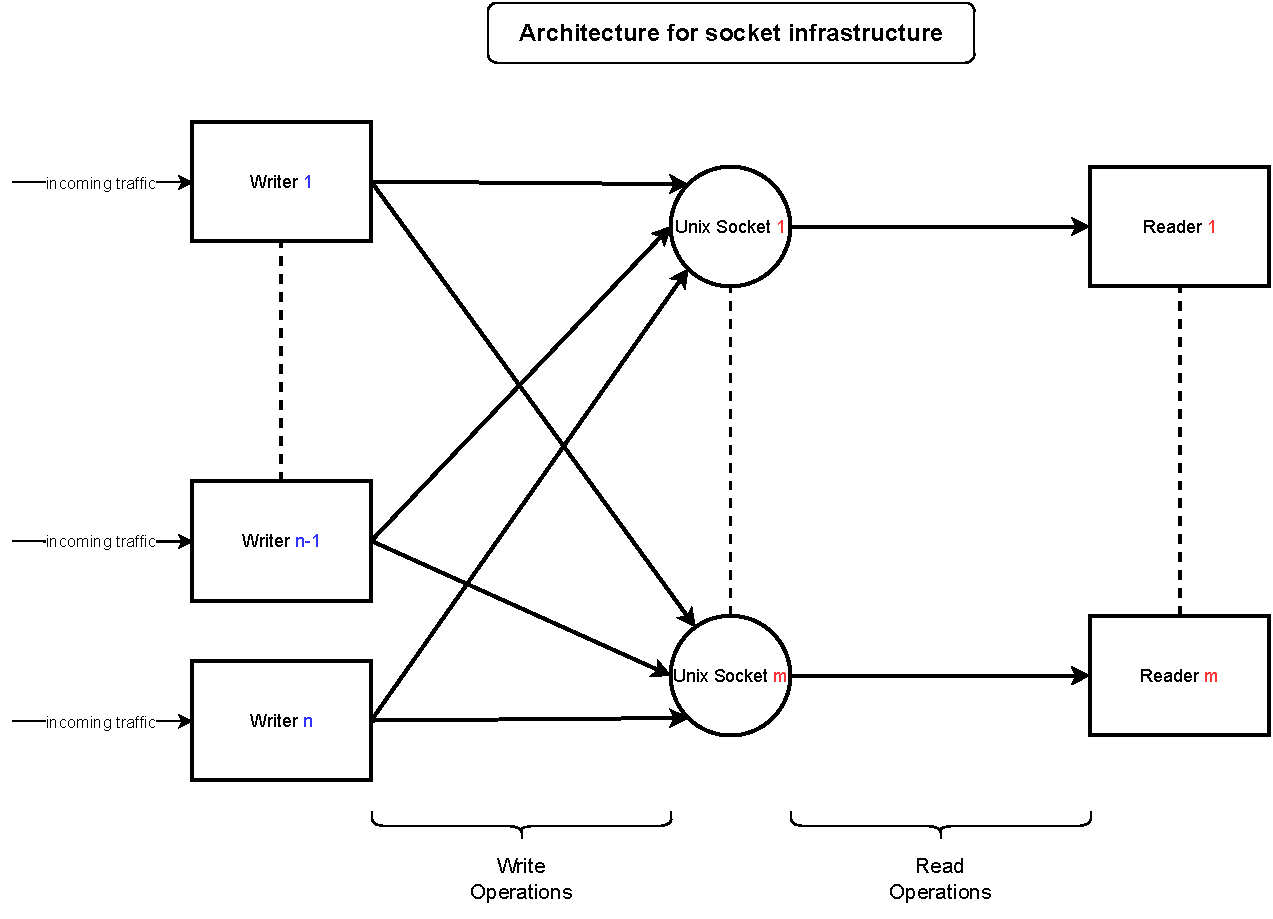
\includegraphics[width=1.2\textwidth]{images/SocketArchitecture.pdf}}
    \caption[General design of socket architecture]{
        Architecture for a n-reader and m-writers scenario using UNIX domain sockets.}
	\label{fig:socket:architecture}
\end{figure}

This figure displays the general data flow using the socket \ac{IPC} type.
Each reader application creates its own UNIX domain socket.
Sockets are bound to a filesystem pathname.
Readers can receive data from their own socket without having to compete or synchronize with other readers for data thanks to the one-to-one mapping between socket and reader.
Meanwhile, writers can also independently write data into sockets without having to communicate with other writer processes.
In order to guarantee that readers receive all data being sent via the socket \ac{IPC} architecture, writers need to periodically recheck for newly opened sockets and always send their data to all available sockets.
This results in the writers having a significant portion of the overhead, needing to resend identical data multiple times.
Minimizing overhead on the reader side is important to maximize the limited computational time that crucial services, such as the \ac{IPS} Simplefail2ban, have available to process incoming log messages.

To preserve the integrity of log messages, the UNIX domain socket needs to retain message boundaries, ruling out the SOCK\_STREAM UNIX domain socket presented in section \ref{cha:UNIXDomainSockets}.
Without the absolute guarantee of reliable behavior in regard to reordering of messages - only present in most UNIX implementations, but not all\cite{man:unixsockets} - SOCK\_DGRAM is unappealing as well.
Therefore, the socket type choice falls on SOCK\_SEQPACKET, a connection-oriented option that retains message-boundaries and sequence.
    
    \acresetall % reset acronym counter
    %
% chapter4.tex
%

\chapter{Implementation}
\label{cha:implementation}
In this chapter, the implementation of the previously discussed design (Reference\@: \ref{sec:Design_and_abstractions}) for the unix domain socket architecture is presented.
This includes an explanation of the write and read API.
All error codes are numeric and defined the file \texttt{io\_ipc.h}

\section{Auxiliary functions and structures}
When utilizing the socket IPC type, some shared resources seen in \ref{alg:variables:shared} need to be set up.
None of these are modified during runtime.

\begin{algorithm}[h!]
    \lstinputlisting[language=c, firstline=18, lastline=22]{code/sock_comm.h}
    \caption[Socket: Shared variables]{Parameters shared between readers and writers.}
    \label{alg:variables:shared}
\end{algorithm}

To ensure that no writer gets stuck continually checking for new sockets, the global variable \texttt{MAX\_AMOUNT\_OF\_SOCKETS} is defined.
This also acts as an upper limit in regards to the amount of reader processes that can attach to the unix domain socket IPC.
The unix domain sockets were bound to the filesystem, resulting in a common path to the location of all sockets needing to be supplied to both readers and writers.
However, this \texttt{SOCKET\_NAME\_TEMPLATE} is not the full path to each socket.
During runtime, each reader process trying to attach will append this name template with their own reader ID.
The reader ID is determined by claiming the first ID not already in use.
Since the length of the reader ID being appended to the \texttt{SOCKET\_NAME\_TEMPLATE} can vary, a maximum length for this template is defined in \texttt{SOCKET\_TEMPLATE\_LENGTH}.

Separating functions utilized by both readers and writers results in an unwieldy API.
Shared usage of functions by both sides is achieved by supplying function calls with the role of the calling process, either \texttt{SOCK\_WRITER} or \texttt{SOCK\_READER}.

\begin{algorithm}[h!]
    \lstinputlisting[language=c, firstline=88, lastline=89]{code/sock_comm.h}
    \caption[Socket: Socket initialization]{Initialization function for both reader and writer processes.}
    \label{alg:sock:init}
\end{algorithm}

Therefore the function initializing communication between processes, \texttt{sock\_init} displayed in \ref{alg:sock:init} only requires a structure of parameters and the role of the calling process.
Defining a union containing both writer and reader structures as seen in \ref{alg:sock:union} allows the user of the API to provide either one as a parameter for the same function.
The actual purpose of \texttt{sock\_init} is to enable connection between writer and readers.
Writers are provided with a list of possible locations of unix domain sockets belonging to reader processes.
Meanwhile, readers are assigned a path, in which they create a unix domain socket.
All sockets are set to be of the type SOCK\_SEQPACKET.

\begin{algorithm}[h!]
    \lstinputlisting[language=c, firstline=75, lastline=78]{code/sock_comm.h}
    \caption[Socket: Union for flexible function calling]{Union containing either the parameters of a writer or reader process.}
    \label{alg:sock:union}
\end{algorithm}

While other IPC types such as shared memory required an orderly detachment of writers and readers, this is not necessary for the socket approach.
Instead, when terminating a reader process, only closure of the corresponding unix domain socket is necessary.
Stopping a writer process currently results in deconstructing the entire unix domain socket architecture.
This results in the functions \texttt{socket\_finalize} and \texttt{socket\_cleanup}, as shown in \ref{alg:sock:finalize} and \ref{alg:sock:cleanup} respectively, being identical in behavior.
In fact, \texttt{socket\_finalize} simply calls \texttt{socket\_cleanup} and was only provided in the socket API to make a seamless replacement of other finalize-style functions when switching IPC types possible.

\begin{algorithm}[h!]
    \lstinputlisting[language=c, firstline=125, lastline=125]{code/sock_comm.h}
    \caption[Socket: Socket finalization]{Initializes cleanup of socket IPC.}
    \label{alg:sock:finalize}
\end{algorithm}

\begin{algorithm}[h!]
    \lstinputlisting[language=c, firstline=135, lastline=135]{code/sock_comm.h}
    \caption[Socket: Socket cleanup]{Cleanup of socket IPC.}
    \label{alg:sock:cleanup}
\end{algorithm}

\section{Write API}
The write API consists out of a single, versatile function \texttt{sock\_writev}.
See \ref{alg_sock} for its definition.

It requires four arguments:
\begin{itemize}
    \item A pointer to an instance of the structure \texttt{sock\_writer\_arg\_t} which will be introduced shortly.
    \item A pointer to an array of \texttt{iovec} structures.
            Each \texttt{iovec} structure defines a separate memory region of variable size, acting as a buffer.
            An entire array of such structures can be represents a vector of memory regions\cite{man:iovec}.
    \item The integer \texttt{invalid\_count} represents the number of log messages located in the iovec array.
    \item Finally, the maximum number of receiving sockets is given via the parameter \texttt{maxNumOfSocks}.
\end{itemize}

\begin{algorithm}[h!]
    \lstinputlisting[language=c, firstline=101, lastline=103]{code/sock_comm.h}
    \caption[Socket: Write API]{Write API for the unix domain socket architecture}
    \label{alg:sock}
\end{algorithm}

When calling \texttt{sock\_writev} the first thing being performed is a check for available unix domain sockets.
This can be considered analogous to checking for new reader because of the strict one-to-one mapping between sockets and readers.
If new sockets were identified, a connection with that socket is established and saved for future calls of this function.
Then, all sockets with an existing connection are sent the data located in the iovec structures using the function \texttt{write}.
On success, the function returns the number of sent messages via the socket IPC.


\section{Read API}
Read API

\section{Features}
Features
    
    \acresetall % reset acronym counter
    %
% chapter5.tex
%

\chapter{Experiments}\label{cha:experiments}
Paul Raatschen has performed a study\cite{raatschen:ipc} concluding that the original Fail2ban process can be improved upon.
It was determined that especially with many clients, Fail2ban struggled to keep up with high incoming traffic rates.
To remedy this issue, a more performant program, Simplefail2ban, was implemented and measured.
An increase in performance was evident.
Simplefail2ban supported two modes of \ac{IPC}.
The disk/file mode was akin to traditional file logging, while the shared memory approach would use a shared memory section to exchange data between processes.
A direct comparison between the already outlined socket approach and previously supported \ac{IPC} types necessitates the measurements in this chapter.

The following chapter details the measurements performed, outlining specifics according to Jain's
``The Art of Computer Systems Performance Analysis: Techniques For Experimental Design, Measurement, Simulation, and Modeling, NY\@: Wiley''\cite{jain:measurement} chapter 2.2.

\section{Test environment}
Two machines, both identical in hardware and software, were used in these experiments.
The first machine, the \ac{DUT}, ran Simplefail2ban and a test application responsible for receiving incoming traffic and reporting clients.
The second machine generated and sent traffic, consisting of both valid and invalid traffic, to the \ac{DUT} using TRex.

\begin{table}[b!]
    \renewcommand{\arraystretch}{1.5}
    \caption[Testbed specs]{Table of Hardware and Software parameters of the testbed.
    The first machine serves as the \ac{DUT}.
	The second machine generates traffic to be sent to the \ac{DUT} via TRex.}\label{tab:specs}
    \centering
    \small
    \begin{tabular}{ll}
        \toprule
        \multicolumn{2}{l}{\textbf{Hardware}} \\ \midrule
        CPU     & 16 $\times$ Intel(R) Xeon(R) Silver 4314 \ac{CPU} @ 2.40GHz \\
        NIC     & Mellanox Technologies MT2892 Family [ConnectX-6 Dx] \\
        RAM     & 128 GB \\ \bottomrule

        \multicolumn{2}{l}{\textbf{Software}} \\ \midrule
        OS          & Debian \ac{GNU}/Linux 11 \\
        Kernel      & 5.10.0-28-amd64 x86\_64 \\
        NIC Driver  & mlx5\_core; Version 5.8-2.0.3 \\
        TRex        & 2.99 (Stateless) \\ \bottomrule
    \end{tabular}
\end{table}

\section{Experimental design}
In his thesis\cite{raatschen:ipc}, Paul Raatschen showed that the shared memory mode of Simplefail2ban outperforms the traditional Fail2ban.
However, it remains unclear if the implementation of this \ac{IPC} type is more performant than other alternatives.
Specifically, the possibility of using UNIX domain sockets as a mode of inter-process communication was not explored.
The following experiments enable a direct comparison between the two \ac{IPC} types.

\noindent
In general, the experiments consist of two participants and a one-sided data exchange.
The \ac{DUT}, or more specifically the application udp\_server, receives a stream of both wanted and unwanted data.
Identifying desired traffic is done by analyzing the message payload.
This is a crude and unrealistic approach to filtering malicious communication requests.
Such a simplification allows the application udp\_server to quickly generate log messages.
Since the goal of this study is to determine the most efficient \ac{IPC} type for Simplefail2ban, it is very plausible that this abstraction does not diminish the findings of this thesis.

\noindent
To compare the differing \ac{IPC} types, a set of performance metrics needs to be established:

\bigskip
\noindent
\textbf{Performance metrics}
\begin{itemize}
    \item Total number of unwanted requests dropped (number of packets)
    \item Total number of unwanted requests dropped, relative to the total amount of unwanted requests sent (percentage)
    \item Number of log messages processed by Simplefail2ban, relative to the number of log messages sent by the test server (percentage)
    \item \ac{CPU} utilization of Simplefail2ban (seconds of \ac{CPU} time)
\end{itemize}
Higher is better for the first three metrics.
The last metric should be minimized for the \ac{DUT} so its services are continually provided to valid clients.

\bigskip
\noindent
The fixed parameters for each of the experiments are the following\@:

\bigskip
\noindent
\textbf{Fixed parameters}
\begin{itemize}
    \item Hardware and Software parameters of the testbed in this table\@:
    \begin{itemize}
        \item \ac{CPU}\@: 16 cores, no hyper-threading enabled
        \item \ac{NIC}\@: Maximum transfer unit is 1500 bytes
        \item TRex\@: One interface, 30 threads
    \end{itemize}
    \item Number of entries in \ac{eBPF} maps for IPv4 \& IPv6\@: 1M
    \item Number of receiving threads used by udp\_server\@: 16
    \item Duration of measurement\@: 300 Seconds
    \item Amount of valid traffic sent\@: 50000 \ac{PPS}
    \item Number of clients sending valid traffic\@: 254
    \item \textbf{Simplefail2ban} parameters\@:
    \begin{itemize}
        \item Number of hash table bins used\@: 6000011
        \item Ban threshold for clients\@: 3
        \item Ban time for clients\@: 30 seconds
        \item Enabling the \ac{Regex} Matching feature of Simplefail2ban (the current implementation does not ban clients correctly when disabled)
        \item For \textbf{shared memory} specifically\@:
        \begin{itemize}
            \item Number of banning threads used\@: 16
            \item Line count for the shared memory buffer segments\@: 1M
            \item Segment count for the shared memory buffer\@: 16
            \item Overwrite feature enabled
            \item Workload stealing feature disabled
        \end{itemize}
        \item For \textbf{sockets} specifically\@:
        \begin{itemize}
            \item Number of banning threads used\@: 16
            \item Number of sockets\@: Same as number of reader processes (either one, or two when utilizing a second reader)
            \item Using default path to sockets created by the application\@: \texttt{tmp/}
            \item Using default socket receive and send buffer size configured on the system\@: 212992 Bytes
        \end{itemize}
        \item For \textbf{file} specifically\@:
        \begin{itemize}
            \item Number of banning threads used\@: 1 (file mode only supports one banning threads)
            \item Buffer size for uring\_getlines\@: 2048
        \end{itemize}
    \end{itemize}
\end{itemize}

\bigskip
\noindent
The factors, or variable parameters, during these experiments were the following\@:

\bigskip
\noindent
\textbf{Factors and their levels}
\begin{itemize}
    \item \ac{IP} stack: IPv4, IPv6 and IPv4/IPv6 mixed
    \item Effects of differing amount of invalid traffic sent: 100k, 1M, 10M, 20M, 30M \ac{PPS}
    \item Effects of differing number of clients sending invalid data: 65534 and 131068
    \begin{itemize}
        \item Range used for 65534 clients: 10.4.0.1 to 10.4.255.254 resulting in clients stemming from 256 subnets (using offset\_fixup of 5 for IPv6 in TRex script).
        \item Range used for 131068 clients: 10.4.0.1 to 10.5.255.252 resulting in clients stemming from 512 subnets (using offset\_fixup of 5 for IPv6 in TRex script).
        \item When using the IPv4/IPv6 \ac{IP} stack, the range for 65534 client is being used twice to generate both a IPv4 and IPv6 stream.
    \end{itemize}
    \item Differing \ac{IPC} type\@: FILE (traditional file-based logging), SHM (using shared memeory), SOCK (using UNIX domain sockets)
    \item For shared memory specifically:
    \begin{itemize}
        \item No 2nd Reader/ Enabling 2nd Reader
    \end{itemize}
    \item For sockets specifically:
    \begin{itemize}
        \item No 2nd Reader/ Enabling 2nd Reader
    \end{itemize}
\end{itemize}

\bigskip
\noindent
To generate the traffic being sent to the \ac{DUT}, TRex scripts are used.
These scripts provide the option to modify the sent traffic according to the factors outlined above.
During these measurements, adapted versions of Paul Raatschens\cite{raatschen:ipc} scripts were used.
To measure most performance metrics, an adaptation of the xdp\_ddos01\_blacklist\_cmdline program was used.
This application originally stems from Florian Mikolajczak master's thesis\cite{mikolajczak:ebpf} and routinely polls the number of dropped and passed packets from a specific \ac{eBPF} map.
It was modified by Paul Raatschen to output values as a \ac{csv} file.
The polled \ac{eBPF} map is ultimately used by Simplefail2ban to ban clients.
\ac{CPU} time was measured via the command top.

\section{Established Simplefail2ban \ac{IPC} types}
Software version changes warrant remeasurement of the shared memory and file \ac{IPC} mode for Simplefail2ban.
These will also be used to evaluate the newly implemented socket mode.

\subsection{Experiment 1a: Simplefail2ban Logfile}
It has already been shown that the file \ac{IPC} type of Simplefail2ban is outperformed by the shared memory mode.
Pure IPv4, IPv6 and a mixed IPv4/IPv6 \ac{IP} stack will be used.
File logging is expected to perform worse than the other \ac{IPC} types discussed in this thesis, and acts as a baseline for the other \ac{IPC} types.
In total, 25 unique measurements were conducted for this experiment.

\subsection{Experiment 1b: Simplefail2ban Shared Memory}
The newly implemented socket approach is intended to be a valid alternative to the shared memory mode of Simplefail2ban.
To enable a direct comparison, measurements for the shared memory mode need to be done under high enough loads, since with lower loads both the socket and shared memory mode are suspected to be performant enough.
All levels of invalid traffic rates are measured individually.
Again, either a pure IPv4, IPv6 or mixed IPv4/IPv6 \ac{IP} stack is utilized.
The most performant features will be used, meaning overwrite is enabled and workload stealing is disabled.
No second reader process is being employed here.
In total, 25 unique measurements were conducted for this experiment

\section{Measuring the socket \ac{API}}
In the following section, thorough variations of factors and their levels are used to evaluate the performance of the socket mode.
Also, heavy workloads are employed to determine how the socket mode performs in worst case scenarios.
This will allow for a direct comparison between socket and shared memory mode.
The data flow in the \ac{DUT} can be seen in \ref{fig:socket:measurement}.

\begin{figure}[h!]
    \centerline{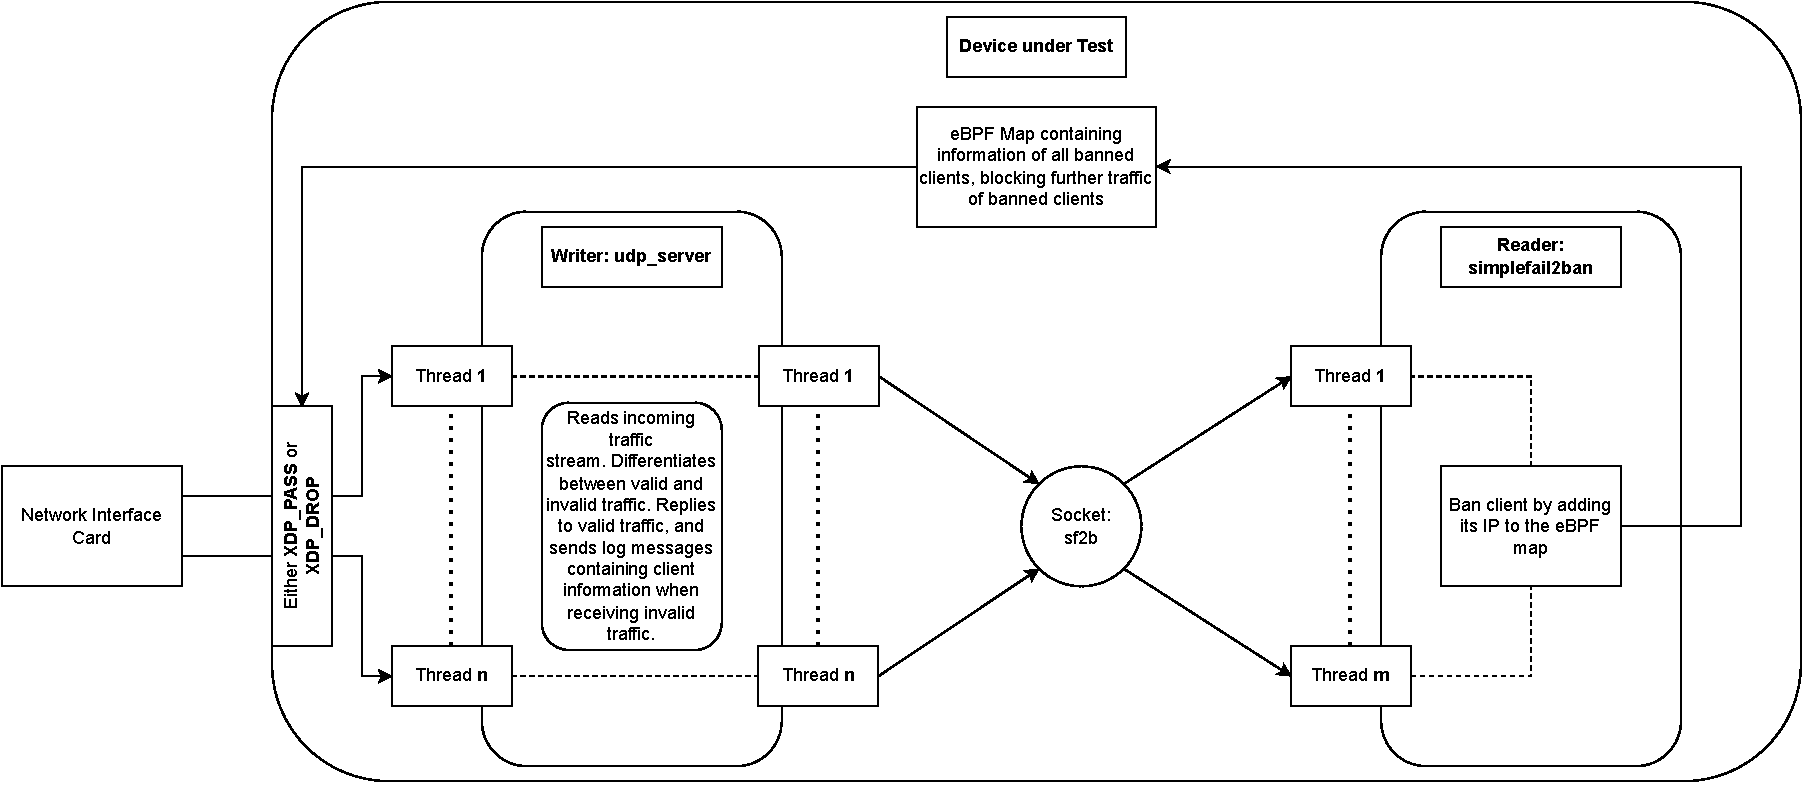
\includegraphics[width=1.2\textwidth]{images/MeasurementArchitecture.pdf}}
    \caption[\ac{DUT} during socket measurements]{
        displays the data flow (left to right) on the \ac{DUT} when enabling sockets as the \ac{IPC} type.
        A packet can either be passed (XDP\_PASS) to the kernel or dropped (XDP\_DROP) before ever reaching the kernel.}
	\label{fig:socket:measurement}
\end{figure}


\subsection{Experiment 2: Simplefail2ban Sockets}
To establish a baseline for the performance of the socket mode, all factors are set to all possible levels in every combination.
The only exception being the possibility of using a second reader process, which will have its own section later.
In total, 25 unique measurements were conducted for this experiment.

\subsection{Experiment 3a: Replication of Simplefail2ban Shared Memory with 2nd Reader}
In order to later compare the socket mode and its option to have a second reader, a baseline measurement needs to be established.
This experiment will be performed with 131068 clients sending invalid data only and no pure IPv4 or IPv6 \ac{IP} stack.
Again, the overwrite feature is enabled while workload stealing is disabled.
The second reader process logs all messages it receives in a log file.
In total, 5 unique measurements were conducted for this experiment.

\subsection{Experiment 3b: Simplefail2ban Sockets with 2nd Reader}
This experiment closely mirrors the experiment 3a.
A total of 131068 clients will send invalid data to the \ac{DUT} with no pure IPv4 or IPv6 \ac{IP} stack.
The shared memory mode inherently supports the possibility of adding a second reader to the shared memory section to read log messages.
There is no such inherent support in the socket mode.
Instead in its current implementation, another read process can be started which will then be assigned its own socket.
This socket will then also receive all log messages.
Consequently, the shared memory mode will likely see a smaller performance loss, since no additional effort is required to send messages to the second reader. 
The second reader process logs all messages it receives in a log file.
In total, 5 unique measurements were conducted for this experiment.

\newpage
\section{Evaluation of Experiments}
The aforementioned experiments can be logically grouped in two categories\@: Baseline measurements and utilization of a second reader.
Baseline measurements are conducted in experiments 1a, 1b and 2, second reader experiments in 3a and 3b.
With 85 performed experiments, a thorough yet not unreasonably long evaluation of each measurement is impossible.
Instead, only especially expressive data will be covered in this section, with any notable or diverging observations being explicitly mentioned.
For full measurement data on all experiments, refer to the repository provided in the sources\cite{git:repoOfThesis}.

\minisec{Meaning of data variables}
In the following section, each graph will be accompanied with an additional table.
This table contains data that is not explicitly expressed otherwise.
A total of six lines are plotted, with two of them belonging to each \ac{IPC} type.
For each \ac{IPC} type (File, Shm, Sock), the total number of packets dropped by the \ac{eBPF} program is denominated via \texttt{XDP\_DROP}.
Similarly, the number of packets passed to the kernel is displayed via \texttt{XDP\_PASS}.
The \texttt{relative drop} represents the percentage of packets dropped relative to the theoretical maximal of dropped packets (represented by \texttt{Best-case drop rate}).
Calculating the relative drop is done with the following formula:
total dropped packets $/ ($experiment duration $*$ invalid traffic rate $-$ number of ban cycles $*$ ban limit $*$ number of malicious clients$)$.
Each ban cycle lasts for 30 seconds.
\texttt{Packets received by udp\_server} lists the number of packets reaching the application udp\_server, while \texttt{Log messages} represents the number of messages sent via the chosen \ac{IPC} type.

\subsection{Baseline measurements}
For this section, data of 75 experiments have been analyzed.

\minisec{Using 65534 clients to send invalid data}
A trend displayed in \ref{fig:data:ipv4:100k:65534} remains prevalent with lower rates of invalid traffic with 65534 clients sending invalid data:
Differences in performance are difficult to spot when graphed.
The table in \ref{fig:data:ipv4:100k:65534} does provide more information.
All \ac{IPC} types perform similarly well in defending the \ac{DoS} attack.

However, one anomaly stands out.
The \texttt{relative drop} of the shared memory \ac{IPC} type is over 100\%.
This happened a total of 21 times over separate measurements, but only when measuring traffic rates of 100k \ac{PPS}.
It is suspected that TRex is unable to provide a reliable stream of packets, but only when starting each measurement call.
Once a steady stream of packets at desired rates has been established, it does remain stable.
Therefore, the number of packets that should be received are higher than the actual incoming traffic rate, resulting in slight inaccuracies when calculating the \texttt{relative drop}.
While not directly apparent at 100k \ac{PPS} due to slight rounding, this discrepancy can be detected by totaling \texttt{XDP\_DROP} and \texttt{XDP\_PASS} up and comparing it to the number of packets that should have theoretically been received.
Unfortunately, this issue is present in all data presented in this thesis and depicts a likely flaw in TRex - not the measurements.

Of note is a stark difference in \ac{CPU} time, with a clearly discernible spike when using the socket \ac{IPC} type, likely cause by extensive context-switches between kernel- and userspace.
All \ac{IPC} types have sent the same number of log messages indicating that, at lower traffic rates, all clients can be banned with the first message they send surpassing the ban limit, regardless of \ac{IPC} type.
This claim is supported by the fact that the log messages coincide with the formula:
number of ban cycles $*$ ban limit $*$ number of malicious clients;
which is the theoretical minimum number of messages needed to successfully ban all clients throughout the duration of the measurement. 
Otherwise, the results are as expected with the file \ac{IPC} type performing worst due to increased latency.

\begin{figure}[!h]
	\centering
	\scriptsize
	\begin{tabular}{c}
    	\centerline{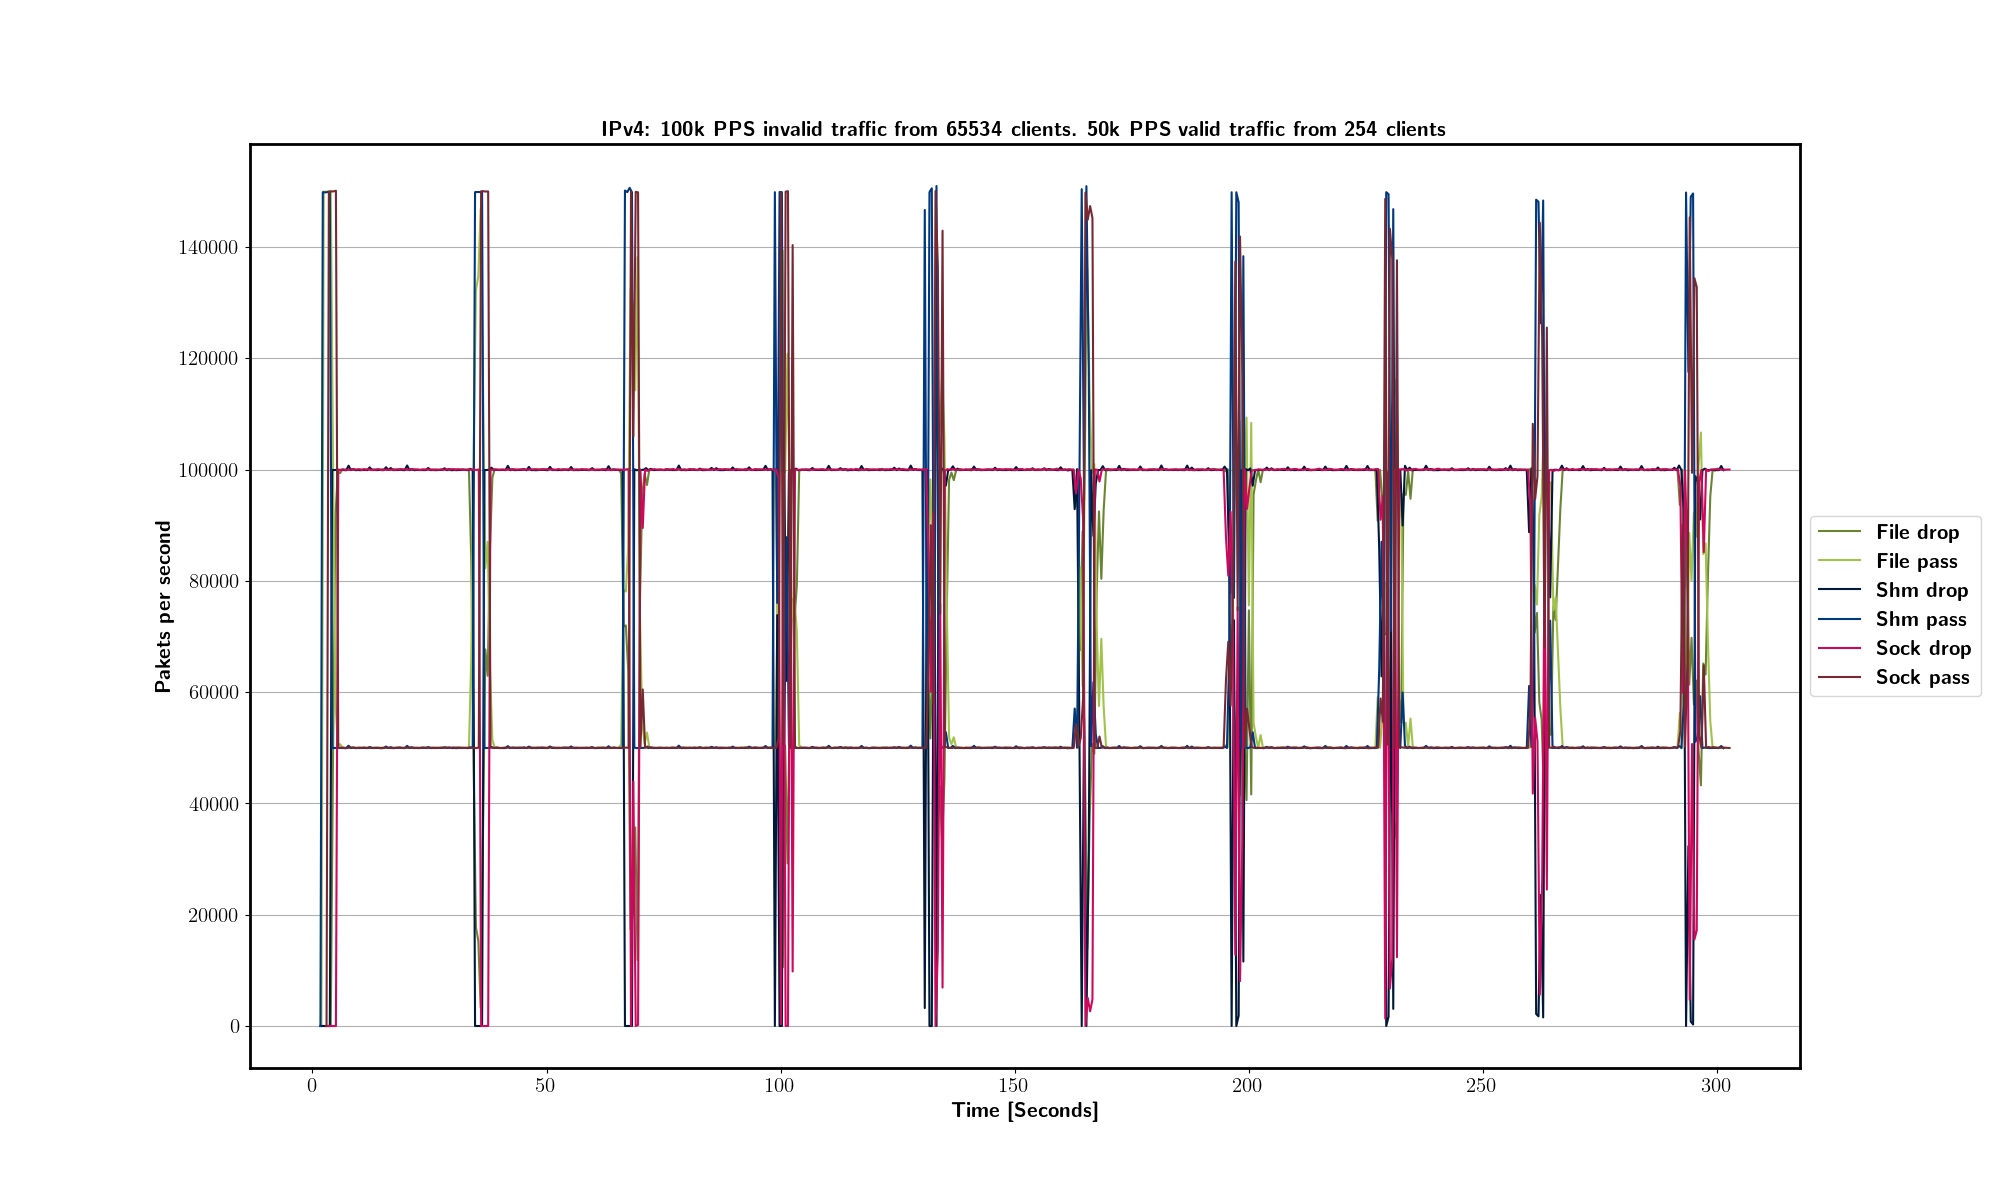
\includegraphics[width=1.2\textwidth]{images/IPv4_100k_65534_1.png}}
	\end{tabular}
	\begin{tabular}{llll}
		\toprule
		\textbf{IPC type} & \textbf{XDP\_DROP [$10^6$]} & \textbf{XDP\_PASS [$10^6$]} & \textbf{Relative drop [\%]} \\ \midrule 
		File & 27,84 & 17,16 & 99,29900071 \\
        Shm & 28,03 & 16,97 & 100,0000036 \\
        Sock & 28,02 & 16,98 & 99,93706566 \\
	\bottomrule
	\end{tabular}
    \begin{tabular}{llll}
		\toprule
		\textbf{IPC type} & \textbf{Packets received by udp\_server [$10^6$]} & \textbf{Log messages [$10^5$]} & \textbf{CPU [seconds]} \\ \midrule 
		File & 16,81 & 19,66 & 04.95 \\
        Shm & 16,97 & 19,66 & 05.94 \\
        Sock & 16,96 & 19,66 & 57.90 \\
	\bottomrule
	\end{tabular}
	\caption[Simplefail2ban, IPv4, 100k \ac{PPS}, 65534 malicious clients]{Total packets sent: 45m. Best-case drop rate: 93,4466\%}
	\label{fig:data:ipv4:100k:65534}
\end{figure}

In \ref{fig:data:ipv4:10m:65534}, the trend of shared memory clearly outperforming other \ac{IPC} types is evident.
Again, differences in plotting the number of dropped and passed packets are to small to be visually decipherable and will be omitted until this changes.
Instead, a clear difference in performance is once again mainly visible in \ac{CPU} time.
The \texttt{relative drop} also reveals that the shared memory \ac{IPC} is performing best, with a lower number of packets being passed to the kernel.
An overall drop in performance measured via \texttt{relative drop} along all \ac{IPC} types was expected.
A generous best-case scenario consists of assuming that all 65534 clients are banned in the same timespan at all incoming traffic rates.
But even then, the inherit latency (even if miniscule) of the \ac{IPS} means that an increase in invalid traffic flow directly correlates with more packets reaching the kernel during each ban cycle.
Therefore, the \texttt{relative drop} rate must inversely correlate with the invalid traffic rate.

\begin{figure}[!h]
	\centering
	\scriptsize
	%\begin{tabular}{c}
    %	\centerline{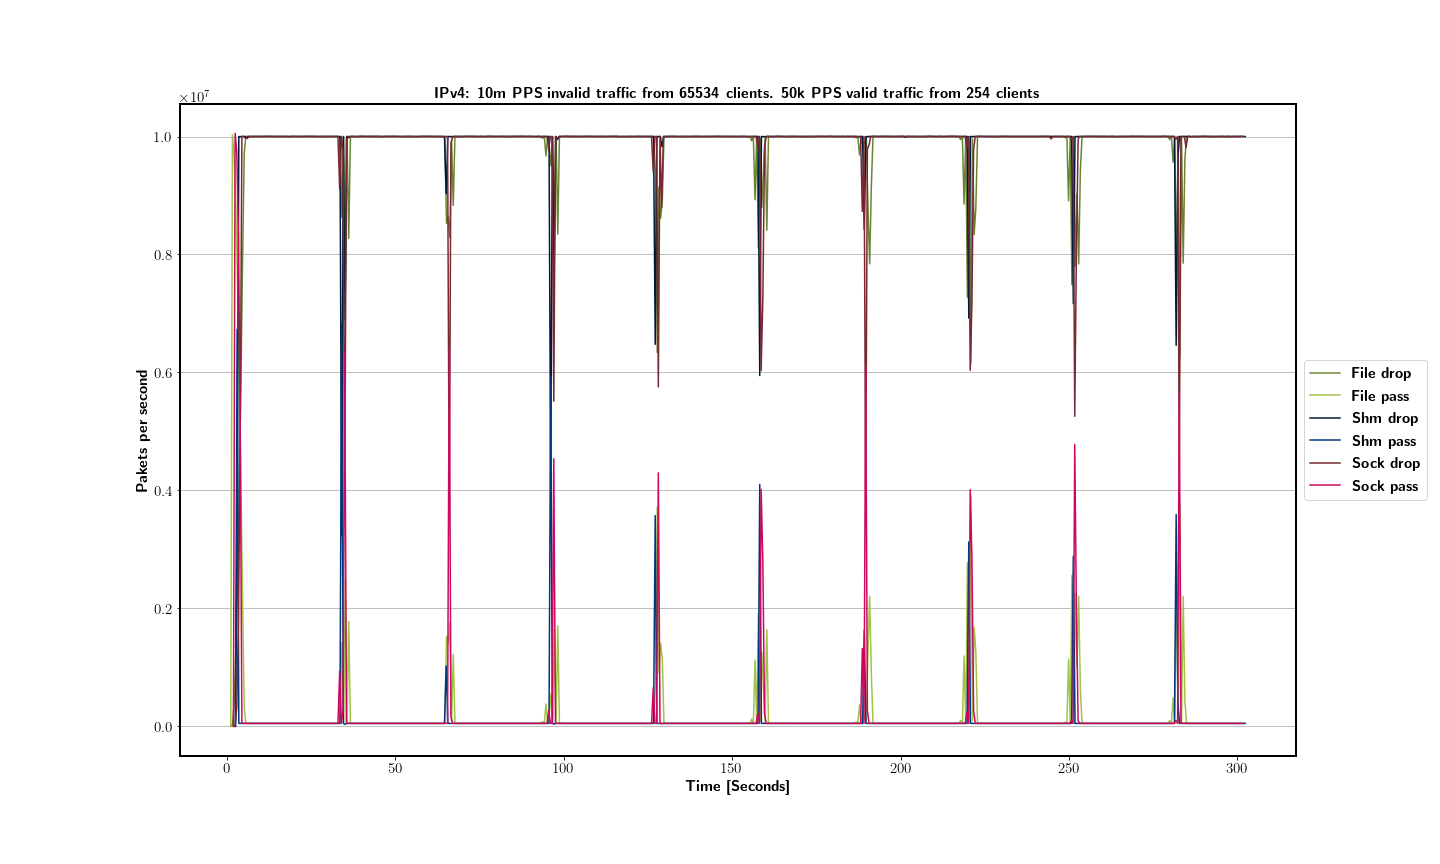
\includegraphics[width=1.2\textwidth]{images/IPv4_10m_65534_1.png}}
	%\end{tabular}
	\begin{tabular}{llll}
		\toprule
		\textbf{IPC type} & \textbf{XDP\_DROP [$10^8$]} & \textbf{XDP\_PASS [$10^6$]} & \textbf{Relative drop [\%]} \\ \midrule 
		File & 29,40 & 75,07 & 98,05973977 \\
        Shm & 29,75 & 37,49 & 99,21848407 \\
        Sock & 29,50 & 61,81 & 98,39458207 \\
	\bottomrule
	\end{tabular}
    \begin{tabular}{llll}
		\toprule
		\textbf{IPC type} & \textbf{Packets received by udp\_server [$10^6$]} & \textbf{Log messages [$10^5$]} & \textbf{CPU [seconds]} \\ \midrule 
		File & 17,51 & 35,10 & 09.69 \\
        Shm & 20,02 & 51,93 & 16.86 \\
        Sock & 17,13 & 25,52 & 76.00 \\
	\bottomrule
	\end{tabular}
	\caption[Simplefail2ban, IPv4, 10m \ac{PPS}, 65534 malicious clients]{Total packets sent: 3015m. Best-case drop rate: 99,934466\%}
	\label{fig:data:ipv4:10m:65534}
\end{figure}

Even with 30m invalid \ac{PPS}, as seen in \ref{fig:data:ipv4:30m:65534}, all \ac{IPC} types successfully defend against the \ac{DoS} attack.
The fact that the file \ac{IPC} type outperforms the socket \ac{IPC} type in terms of \texttt{relative drop} rate is especially noteworthy.
File mode also outperforms shared memory and socket mode on \ac{CPU} usage, which was not expected due to the traditionally high latency of file-based logging approaches.
With the high rate of incoming traffic during a ban cycle, the application udp\_server has to wait on the \ac{IPC} to be able to submit more log messages to Simplefail2ban.
This results in the system being unable to submit a substantial number of packets to udp\_server.
While not explicitly documented in this thesis, these numbers are available in the repository\cite{git:repoOfThesis}.
The difference in packets received by udp\_server and number of passed packets correlates exactly with this observation.
Measuring the number of packets unable to be submitted to udp\_server was done by checking the file \texttt{/proc/net/udp6} on the \ac{DUT}.

A mutual feature of these three measurements is the direct correlation between \texttt{relative drop} rate and number of \texttt{packets received by udp\_server}.
Better performing \ac{IPC} types generally receive more packets despite the fact that they block invalid traffic at an increased rate.
This is explainable through the inability of the system to supply new packets to udp\_server while it is still waiting on the \ac{IPC} architecture to deliver data to the \ac{IPS}.
\ac{IPC} types with lower latency and higher bandwidth can log more messages during the short influx of packets during each ban cycle.
Hence, udp\_server can receive more packets from the system.
These attributes also result in higher \texttt{relative drop} rates, thus causing this observation.

\begin{figure}[!h]
	\centering
	\scriptsize
	%\begin{tabular}{c}
    %	\centerline{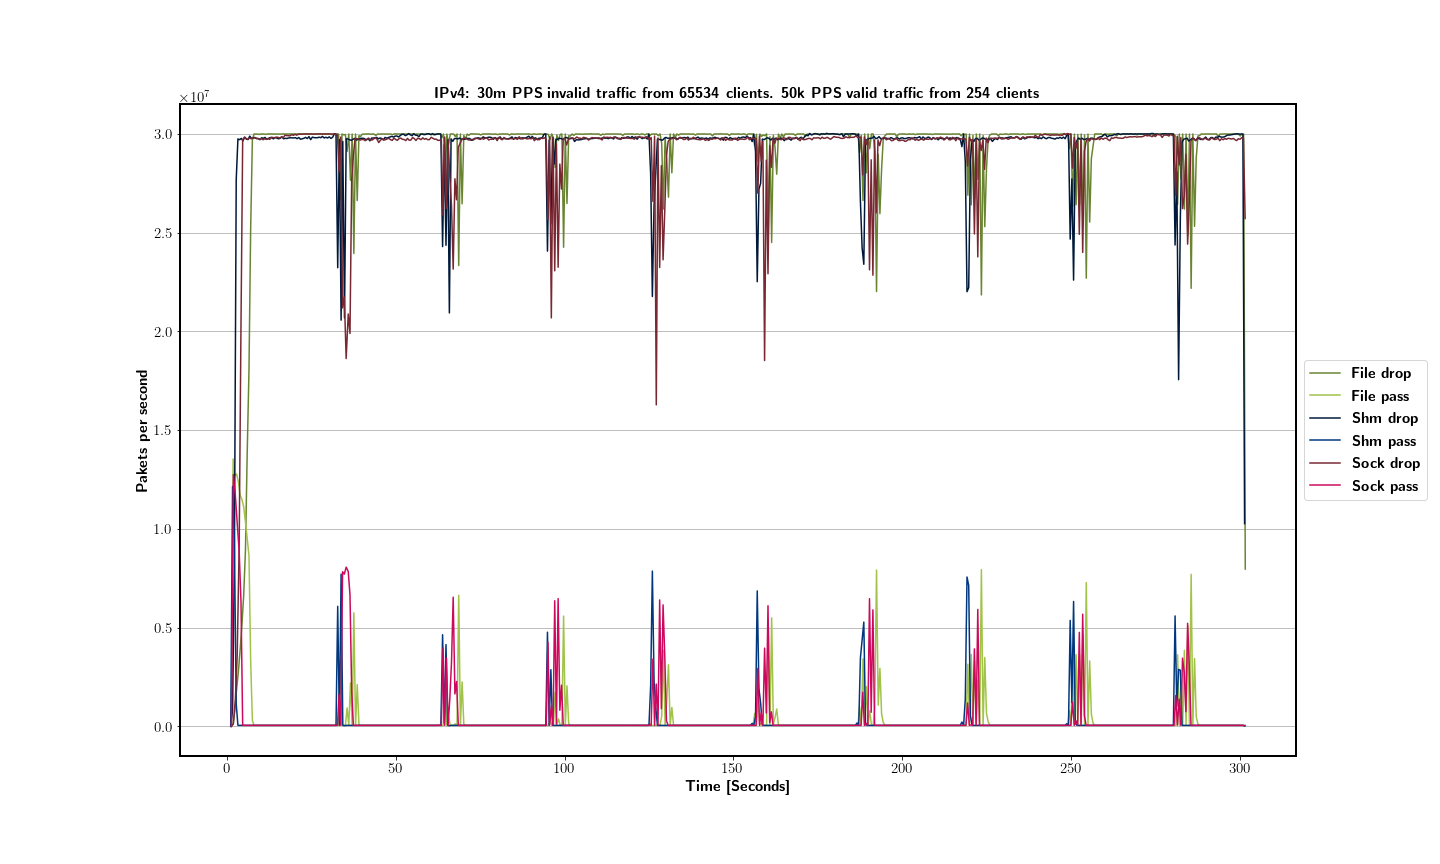
\includegraphics[width=1.2\textwidth]{images/IPv4_30m_65534_1.png}}
	%\end{tabular}
	\begin{tabular}{llll}
		\toprule
		\textbf{IPC type} & \textbf{XDP\_DROP [$10^8$]} & \textbf{XDP\_PASS [$10^6$]} & \textbf{Relative drop [\%]}\\ \midrule 
		File & 87,75 & 159,82 & 97,52375345 \\
        Shm & 88,30 & 87,23 & 98,13105047 \\
        Sock & 87,45 & 139,42 & 97,18179422 \\
	\bottomrule
	\end{tabular}
    \begin{tabular}{llll}
		\toprule
		\textbf{IPC type} & \textbf{Packets received by udp\_server [$10^6$]} & \textbf{Log messages [$10^5$]} & \textbf{CPU [seconds]} \\ \midrule 
		File & 17,48 & 40,72 & 16.55 \\
        Shm & 21,39 & 69,92 & 39.08 \\
        Sock & 16,92 & 31,62 & 138.85 \\
	\bottomrule
	\end{tabular}
	\caption[Simplefail2ban, IPv4, 30m \ac{PPS}, 65534 malicious clients]{Total packets sent: 9015m. Best-case drop rate: 99,97815533\%}
	\label{fig:data:ipv4:30m:65534}
\end{figure}

Figure \ref{fig:data:ipv6:30m:65534} displays \ac{IPC} types under 30m invalid \ac{PPS} from 65534 different clients using IPv6 addresses in contrast to the previously used IPv4 addresses.
Usage of different \ac{IP} stacks had little impact on the overall results of this thesis, which is why lower traffic rates for IPv6 are omitted.

As expected, the file \ac{IPC} type performed worst, with shared memory performing best.
However, contradicting expectations, the socket and shared memory \ac{IPC} types performed better when dealing with IPv6 instead of IPv4 addresses.
This is surprising since no changes in general behavior are expected in either udp\_server or Simplefail2ban with one exception: The \ac{Regex} matching feature.
In theory, IPv6 banning should be less performant than using IPv4, because IPv6 addresses are longer than IPv4 addresses.
Reading these addresses out of the log messages received by Simplefail2ban using the \ac{Regex} matching feature should require more time.
This idea is supported by the increase in \ac{CPU} time across all \ac{IPC} types compared to figure \ref{fig:data:ipv4:30m:65534} using IPv4.
However, an increase in performance can be measured in almost all experiments using IPv6 instead of IPv4.
What exactly causes this abnormality is unclear.

\begin{figure}[!h]
	\centering
	\scriptsize
	%\begin{tabular}{c}
    %	\centerline{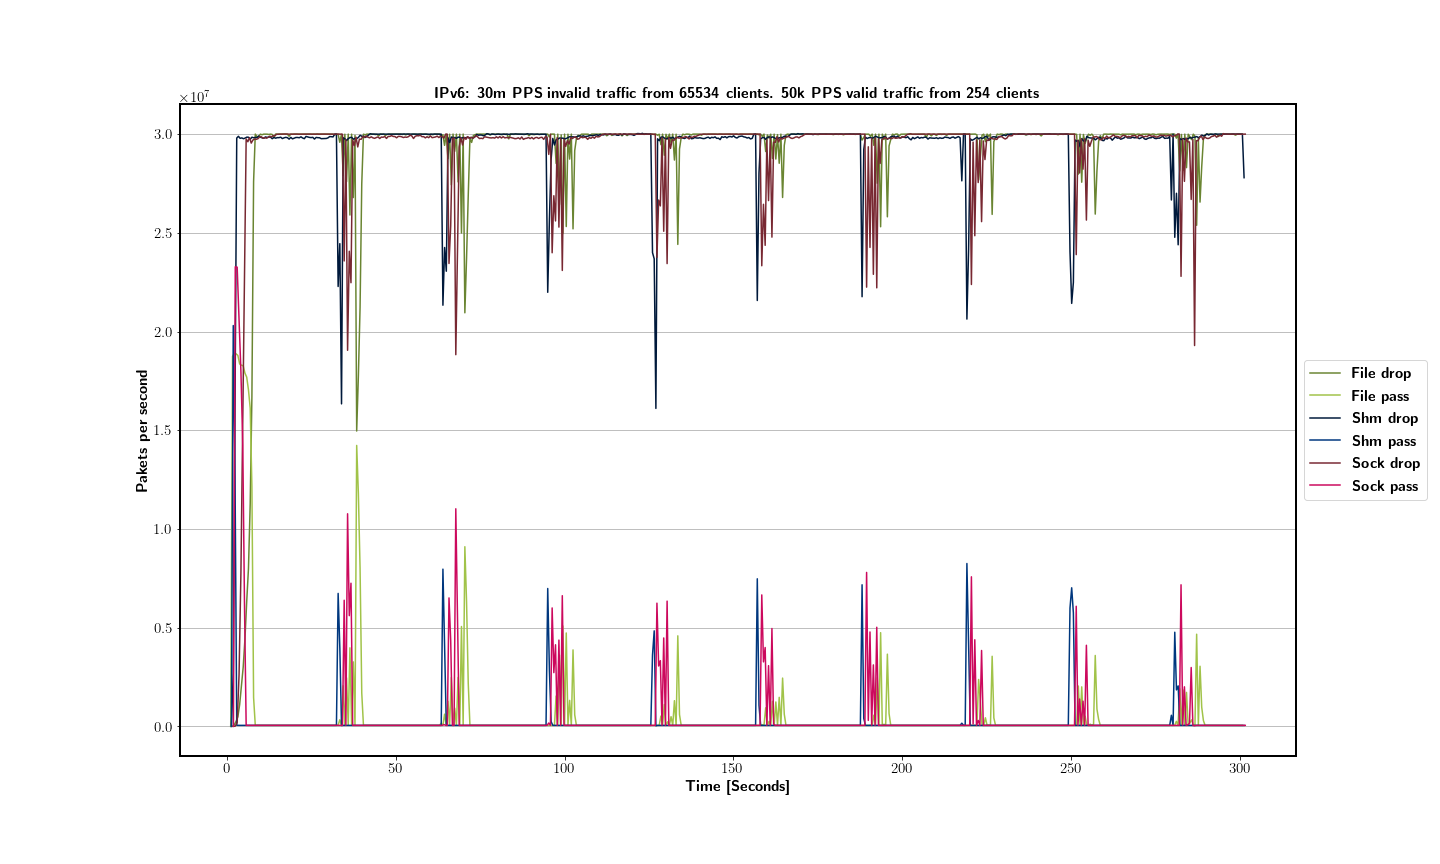
\includegraphics[width=1.2\textwidth]{images/IPv6_30m_65534_1.png}}
	%\end{tabular}
	\begin{tabular}{llll}
		\toprule
		\textbf{IPC type} & \textbf{XDP\_DROP [$10^8$]} & \textbf{XDP\_PASS [$10^6$]} & \textbf{Relative drop [\%]} \\ \midrule 
		File & 87,41 & 211,05 & 97,14091697 \\
        Shm & 88,63 & 85,55 & 98,50239609 \\
        Sock & 87,77 & 170,03 & 97,54838057 \\
	\bottomrule
	\end{tabular}
    \begin{tabular}{llll}
		\toprule
		\textbf{IPC type} & \textbf{Packets received by udp\_server [$10^6$]} & \textbf{Log messages [$10^5$]} & \textbf{CPU [seconds]} \\ \midrule 
		File & 17,20 & 38,73 & 22.51 \\
        Shm & 21,79 & 72,38 & 46.03 \\
        Sock & 16,92 & 30,04 & 149.69 \\
	\bottomrule
	\end{tabular}
	\caption[Simplefail2ban, IPv6, 30m \ac{PPS}, 65534 malicious clients]{Total packets sent: 9015m. Best-case drop rate: 99,97815533\%}
	\label{fig:data:ipv6:30m:65534}
\end{figure}

\minisec{Using 131068 clients to send invalid data}
When using 131068 clients to send invalid data, changes in performance become visible when plotted.
Figure \ref{fig:data:ipv4:100k:131068} displays only 100k invalid \ac{PPS}, yet the file \ac{IPC} type struggles to quickly ban all clients.
In contrast, both socket and shared memory seem to perform quite similarly across all statistics except for \ac{CPU} time.
Here, the socket \ac{IPC} type occupies the \ac{CPU} almost ten times longer than shared memory, again likely due to extensive context-switches between kernel- and userspace.

\begin{figure}[!h]
	\centering
	\scriptsize
	\begin{tabular}{c}
    	\centerline{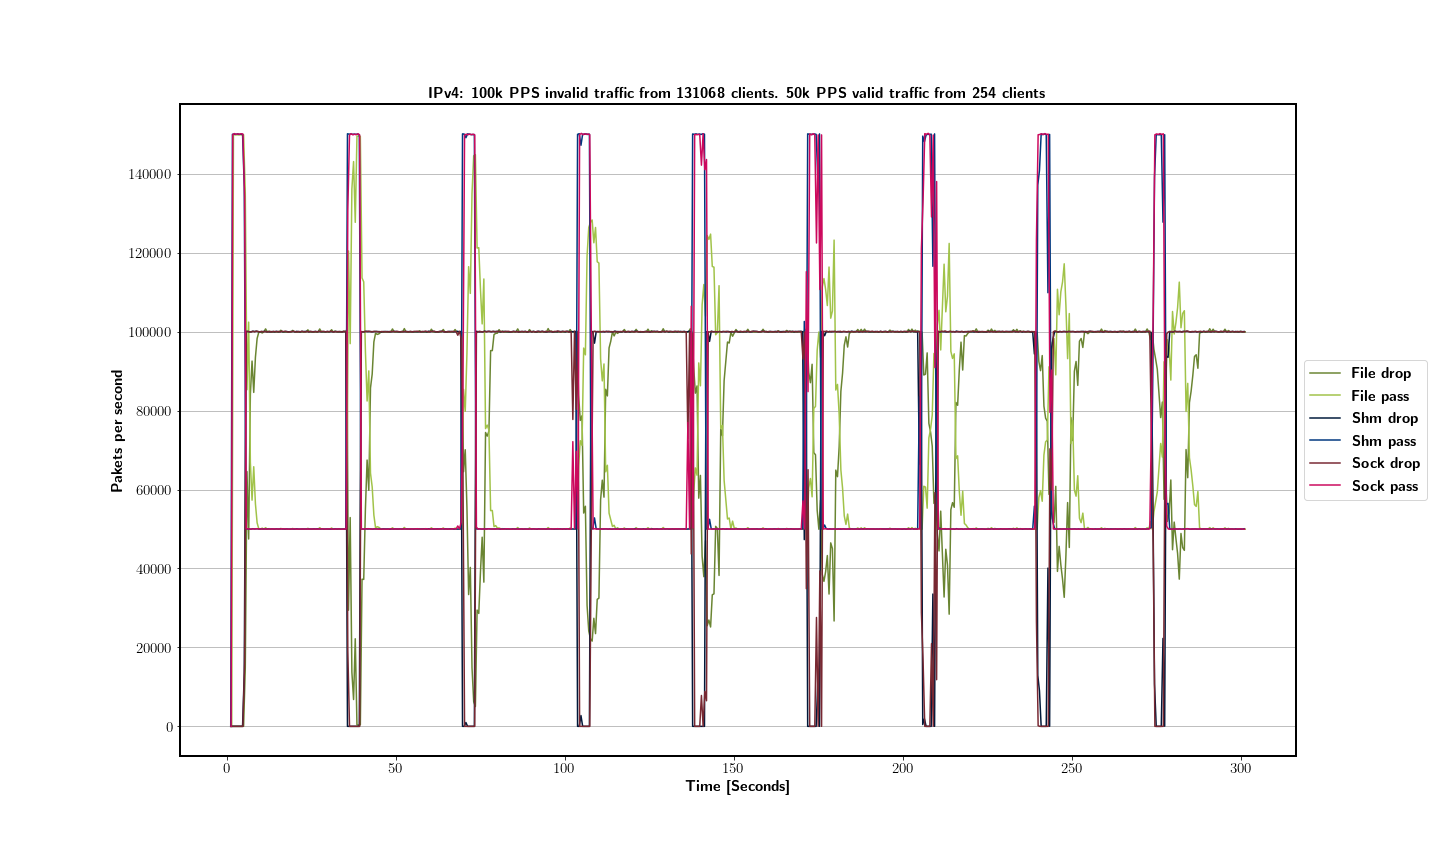
\includegraphics[width=1.2\textwidth]{images/IPv4_100k_131068_1.png}}
	\end{tabular}
	\begin{tabular}{llll}
		\toprule
		\textbf{IPC type} & \textbf{XDP\_DROP [$10^6$]} & \textbf{XDP\_PASS [$10^6$]} & \textbf{Relative drop [\%]} \\ \midrule 
		File & 25,99 & 19,01 & 99,69409958 \\
        Shm & 26,46 & 18,54 & 101,5083842 \\
        Sock & 26,44 & 18,56 & 101,4395334 \\
	\bottomrule
	\end{tabular}
    \begin{tabular}{llll}
		\toprule
		\textbf{IPC type} & \textbf{Packets received by udp\_server [$10^6$]} & \textbf{Log messages [$10^5$]} & \textbf{CPU [seconds]} \\ \midrule 
		File & 18,16 & 35,39 & 08.34 \\
        Shm & 18,54 & 35,39 & 10.14 \\
        Sock & 18,53 & 35,39 & 100.40 \\
	\bottomrule
	\end{tabular}
	\caption[Simplefail2ban, IPv4, 100k \ac{PPS}, 131068 malicious clients]{Total packets sent: 45m. Best-case drop rate: 86,8932\%}
	\label{fig:data:ipv4:100k:131068}
\end{figure}

At invalid traffic rates of 10m \ac{PPS}, displayed in figure \ref{fig:data:ipv4:10m:131068}, drastic changes are noticeable.
Firstly, shared memory does outperform both the socket and file \ac{IPC} type in \texttt{relative drop} rate.
Also, the latency of each \ac{IPC} type is clearly visible in the provided graph via their drasticly shifted spike of dropped packets each ban cycle.
The shared memory \ac{IPC} type both starts and ends its ban cycles before the socket and file \ac{IPC} type.
Unexpectedly, the socket \ac{IPC} type still outperforms the file \ac{IPC} type in \texttt{relative drop} rate.
A general delay of each ban cycle is visible too.
The second to last ban cycle, which should start at 240 seconds, starts late at about 250 seconds.
This delay is present in all \ac{IPC} types. 
It is likely caused by the unbanning thread of Simplefail2ban having to handle 131068 clients, resulting in them being banned, on average, slightly longer than the intended 30 seconds.

\begin{figure}[!h]
	\centering
	\scriptsize
	\begin{tabular}{c}
    	\centerline{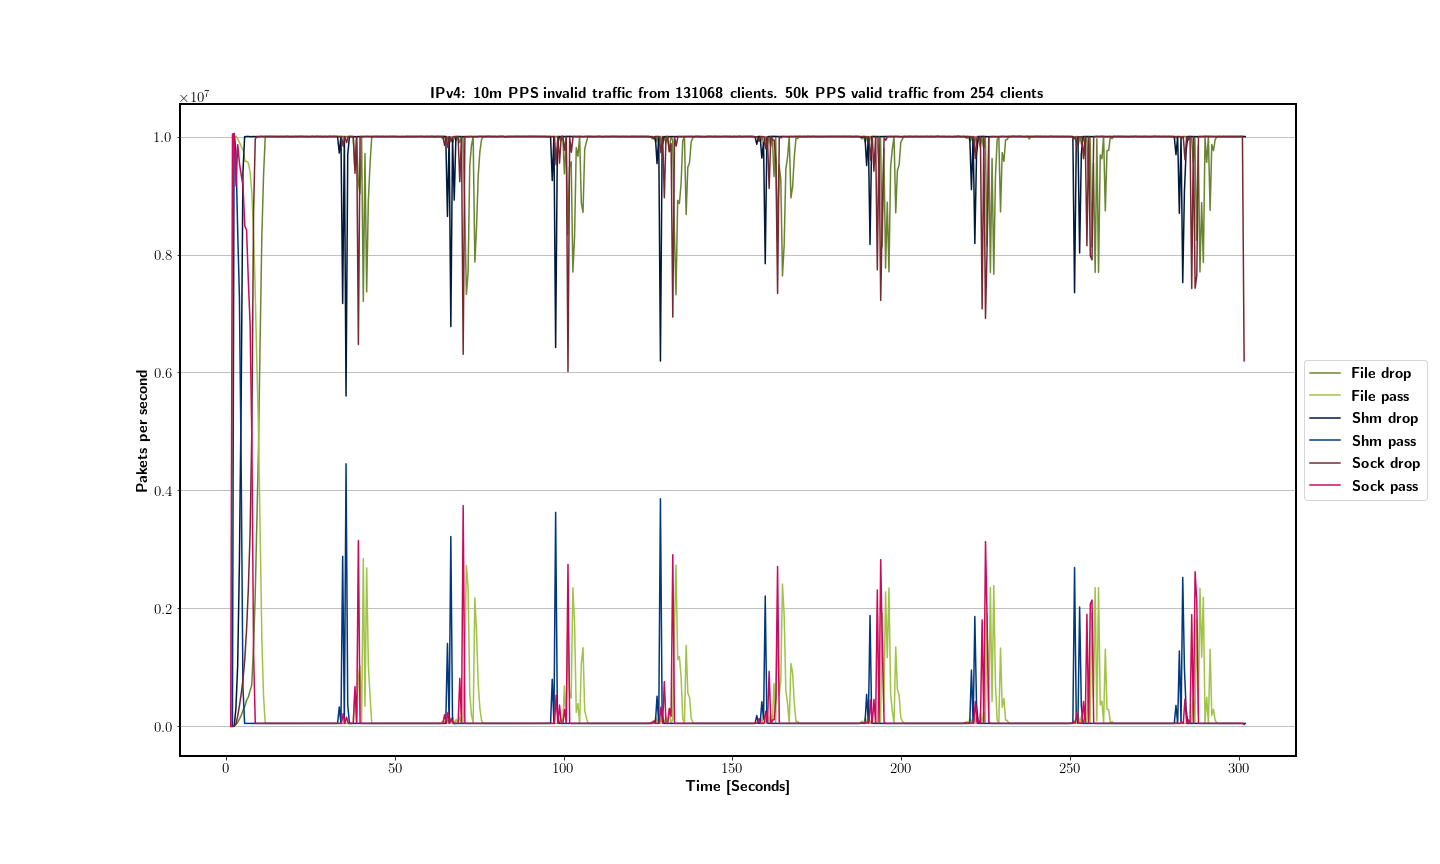
\includegraphics[width=1.2\textwidth]{images/IPv4_10m_131068_1.png}}
	\end{tabular}
	\begin{tabular}{llll}
		\toprule
		\textbf{IPC type} & \textbf{XDP\_DROP [$10^8$]} & \textbf{XDP\_PASS [$10^6$]} & \textbf{Relative drop [\%]} \\ \midrule 
		File & 28,77 & 136,15 & 96,03486581 \\
        Shm & 29,54 & 58,36 & 98,60515631 \\
        Sock & 29,16 & 95,52 & 97,33669129 \\
	\bottomrule
	\end{tabular}
    \begin{tabular}{llll}
		\toprule
		\textbf{IPC type} & \textbf{Packets received by udp\_server [$10^6$]} & \textbf{Log messages [$10^5$]} & \textbf{CPU [seconds]} \\ \midrule 
		File & 19,31 & 63,90 & 19.39 \\
        Shm & 25,40 & 107,54 & 29.47 \\
        Sock & 19,02 & 47,67 & 133.54 \\
	\bottomrule
	\end{tabular}
	\caption[Simplefail2ban, IPv4, 10m \ac{PPS}, 131068 malicious clients]{Total packets sent: 3015m. Best-case drop rate: 99,868932\%}
	\label{fig:data:ipv4:10m:131068}
\end{figure}

At 30m invalid \ac{PPS}, seen in figure \ref{fig:data:ipv4:30m:131068}, the file \ac{IPC} type starts and finishes its ban cycles later than other \ac{IPC} types.
While the shared memory and socket \ac{IPC} type start almost simultaneously, sockets require longer to finish a full ban cycle.
Differences in \ac{CPU} time are prominent, with the socket \ac{IPC} performing worst and file \ac{IPC} performing best according to the \texttt{relative drop} rate.
A general trend found in all measurements presented is the low throughput of the socket \ac{IPC} type.
Here, it is especially pronounced with the shared memory \ac{IPC} type managing to transmit almost double the amount of \texttt{log messages}.

\begin{figure}[!h]
	\centering
	\scriptsize
	\begin{tabular}{c}
    	\centerline{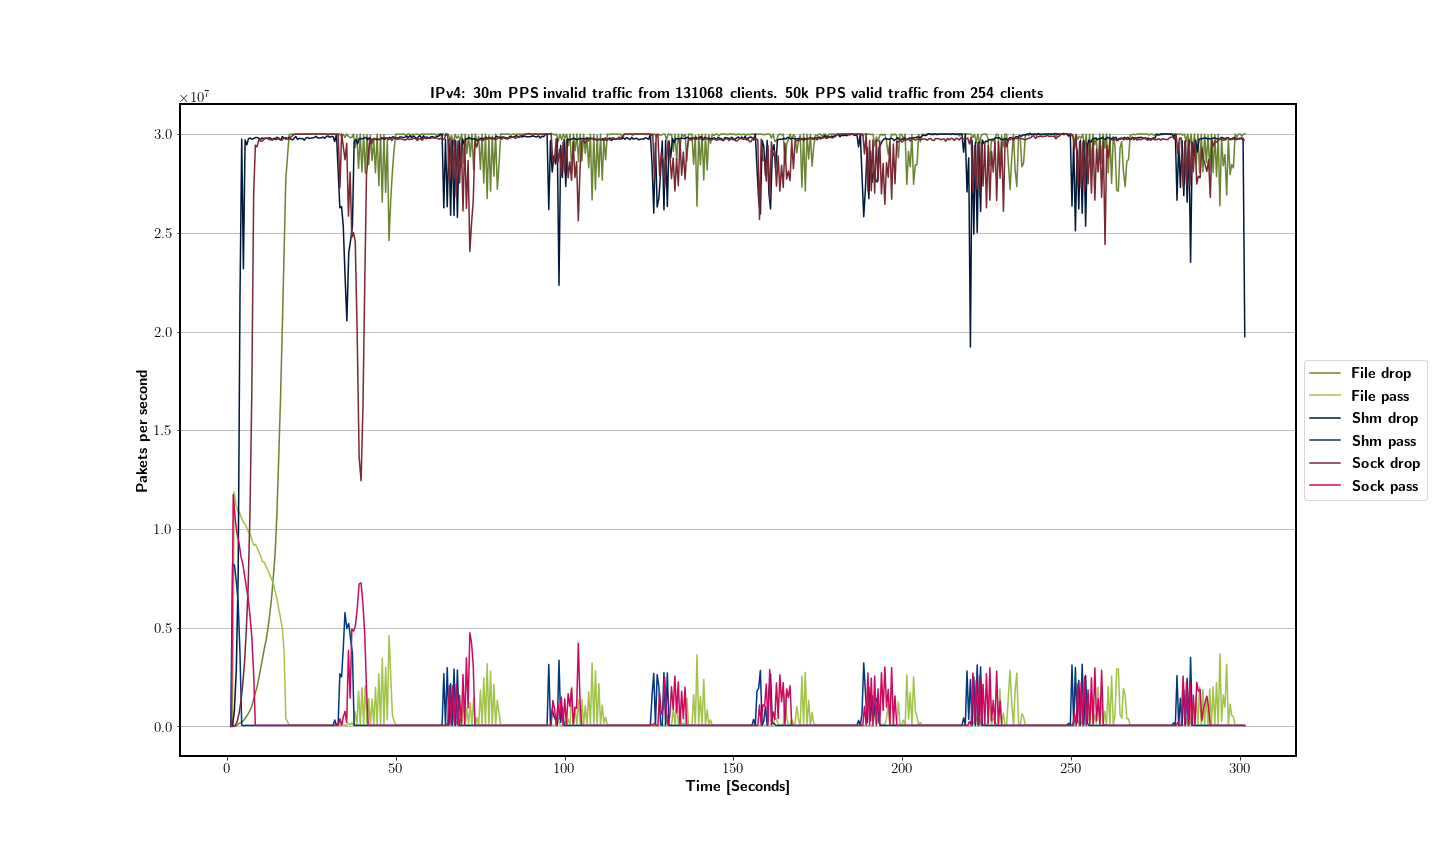
\includegraphics[width=1.2\textwidth]{images/IPv4_30m_131068_2.png}}
	\end{tabular}
	\begin{tabular}{llll}
		\toprule
		\textbf{IPC type} & \textbf{XDP\_DROP [$10^8$]} & \textbf{XDP\_PASS [$10^6$]} & \textbf{Relative drop [\%]} \\ \midrule 
		File & 85,02 & 238,30 & 94,51036756 \\
        Shm & 87,57 & 104,14 & 97,33826458 \\
        Sock & 86,12 & 180,89 & 95,73084169 \\
	\bottomrule
	\end{tabular}
    \begin{tabular}{llll}
		\toprule
		\textbf{IPC type} & \textbf{Packets received by udp\_server [$10^6$]} & \textbf{Log messages [$10^5$]} & \textbf{CPU [seconds]} \\ \midrule 
		File & 18,04 & 74,39 & 38.99 \\
        Shm & 25,32 & 115,04 & 71.92 \\
        Sock & 18,33 & 59,26 & 323.02 \\
	\bottomrule
	\end{tabular}
	\caption[Simplefail2ban, IPv4, 30m \ac{PPS}, 131068 malicious clients]{Total packets sent: 9015m. Best-case drop rate: 99,95631067\%}
	\label{fig:data:ipv4:30m:131068}
\end{figure}

Switching to IPv6 at a rate of 30m invalid \ac{PPS} does not yield any fundamentally different results: \ref{fig:data:ipv6:30m:131068}.
Again, performance of all \ac{IPC} types improves slightly, still with no known cause.
Shared memory performs best, with the file \ac{IPC} type performing worst.
The direct correlation between \texttt{relative drop} rate and \texttt{packets received by udp\_server} is also still present.

\begin{figure}[!h]
	\centering
	\scriptsize
	%\begin{tabular}{c}
    %	\centerline{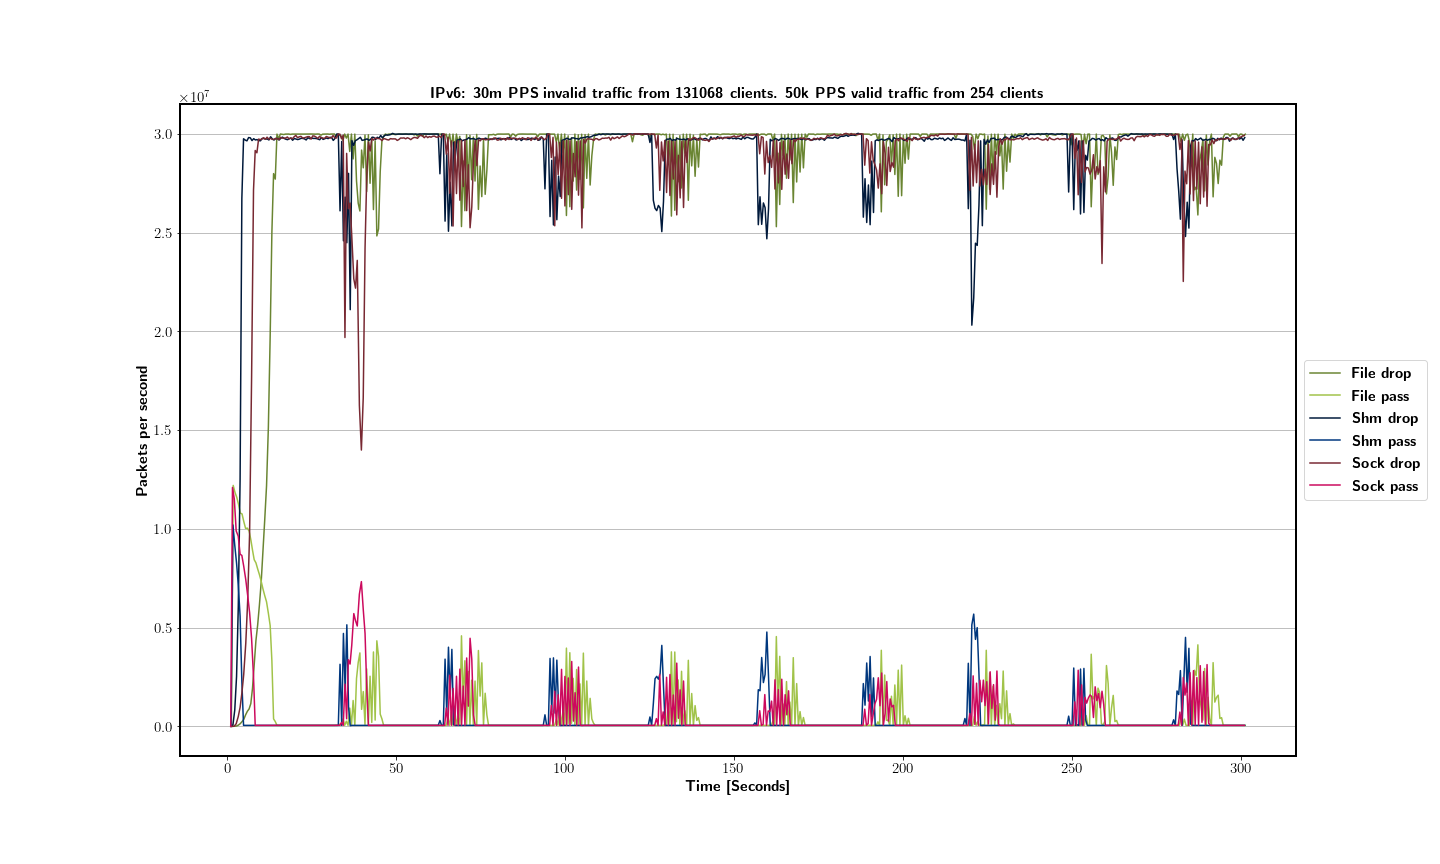
\includegraphics[width=1.2\textwidth]{images/IPv6_30m_131068_1.png}}
	%\end{tabular}
	\begin{tabular}{llll}
		\toprule
		\textbf{IPC type} & \textbf{XDP\_DROP [$10^8$]} & \textbf{XDP\_PASS [$10^6$]} & \textbf{Relative drop [\%]} \\ \midrule 
		File & 85,73 & 228,07 & 95,29278185 \\
        Shm & 87,60 & 109,08 & 97,37706621 \\
        Sock & 86,21 & 177,33 & 95,82614459 \\
	\bottomrule
	\end{tabular}
    \begin{tabular}{llll}
		\toprule
		\textbf{IPC type} & \textbf{Packets received by udp\_server [$10^6$]} & \textbf{Log messages [$10^5$]} & \textbf{CPU [seconds]} \\ \midrule 
		File & 17,90 & 69,14 & 38.41 \\
        Shm & 25,08 & 111,45 & 74.71 \\
        Sock & 18,67 & 61,84 & 317.37 \\
	\bottomrule
	\end{tabular}
	\caption[Simplefail2ban, IPv6, 30m \ac{PPS}, 131068 malicious clients]{Total packets sent: 9015m. Best-case drop rate: 99,95631067\%}
	\label{fig:data:ipv6:30m:131068}
\end{figure}

When using a mixed \ac{IP} stack, two streams of invalid data were configured in TRex: One being IPv4, the other being IPv6.
Both streams were producing exactly 50\% of the invalid traffic and consisted out of 65534 clients each.
Naturally, no single client sent both IPv4 and IPv6 packets.
The most expressive measurement is displayed in \ref{fig:data:ipv4v6:30m:131068} with 30m invalid \ac{PPS}.
Expectations were that the \texttt{relative drop} rate for all \ac{IPC} types would land firmly between the equivalent measurements using IPv4 and IPv6.
However, this is not the case.
The figure \ref{fig:data:ipv4v6:30m:131068} does not display this property.
In fact, no other measurements using a mixed \ac{IP} stack definitively exhibit this property.
Here, in figure \ref{fig:data:ipv4v6:30m:131068}, the shared memory and socket \ac{IPC} types outperform the measurement utilizing pure IPv6 displayed in \ref{fig:data:ipv6:30m:131068}.
Though, most measurements still outperform their pure IPv4 counterpart at a minimum.
But performance regarding their pure IPv6 counterpart is not definitive, the variance between measurements is too severe.

\begin{figure}[!h]
	\centering
	\scriptsize
	%\begin{tabular}{c}
    %	\centerline{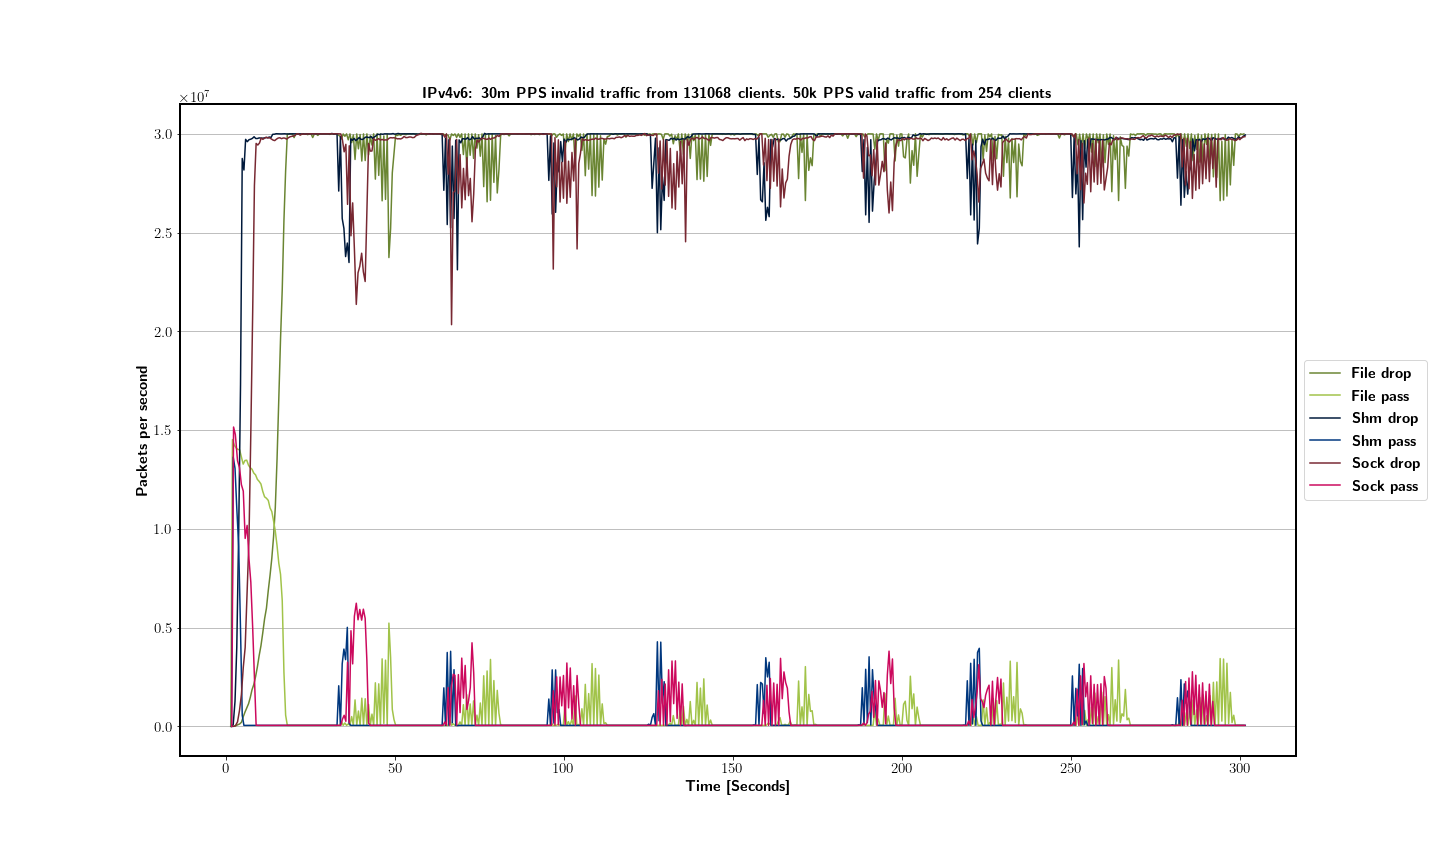
\includegraphics[width=1.2\textwidth]{images/IPv4v6_30m_131068_2.png}}
	%\end{tabular}
	\begin{tabular}{llll}
		\toprule
		\textbf{IPC type} & \textbf{XDP\_DROP [$10^8$]} & \textbf{XDP\_PASS [$10^6$]} & \textbf{Relative drop [\%]} \\ \midrule 
		File & 85,12 & 286,15 & 94,61335186 \\
        Shm & 88,02 & 105,83 & 97,84149307 \\
        Sock & 86,30 & 212,81 & 95,93428297 \\
	\bottomrule
	\end{tabular}
    \begin{tabular}{llll}
		\toprule
		\textbf{IPC type} & \textbf{Packets received by udp\_server [$10^6$]} & \textbf{Log messages [$10^5$]} & \textbf{CPU [seconds]} \\ \midrule 
		File & 17,69 & 70,65 & 47.15 \\
        Shm & 25,13 & 111,62 & 94.64 \\
        Sock & 18,00 & 59,85 & 353.34 \\
	\bottomrule
	\end{tabular}
	\caption[Simplefail2ban, IPv4v6, 30m \ac{PPS}, 131068 malicious clients]{Total packets sent: 9015m. Best-case drop rate: 99,95631067\%}
	\label{fig:data:ipv4v6:30m:131068}
\end{figure}

\subsection{2nd reader measurements}
Initially, data of 10 experiments have been analyzed for this section.
At 100k invalid \ac{PPS}, performance of both the shared memory and socket \ac{IPC} types was almost identical.
The only exception is the \ac{CPU} time in which the socket \ac{IPC} performed up to six times worse than shared memory.
The results become interesting when increasing invalid traffic rate to 1m \ac{PPS}, a seen in figure \ref{fig:data:ipv4v6:1m:131068:2nd}.
The graph displays a clear delay between the ban cycles of the shared memory and socket \ac{IPC} types.
Still, both modes are able to supply both the \ac{IPS} Simplefail2ban and a slower reader process with data while defending against the \ac{DoS} attack.
Again, \ac{CPU} time of the socket \ac{IPC} type is significantly higher than its shared memory counterpart.
The \texttt{relative drop} rate is also worse by about 2 percent (equal to 6,3M more packets reaching the kernel over the duration of the measurement), with fewer messages logged.

\begin{figure}[!h]
	\centering
	\scriptsize
	\begin{tabular}{c}
    	\centerline{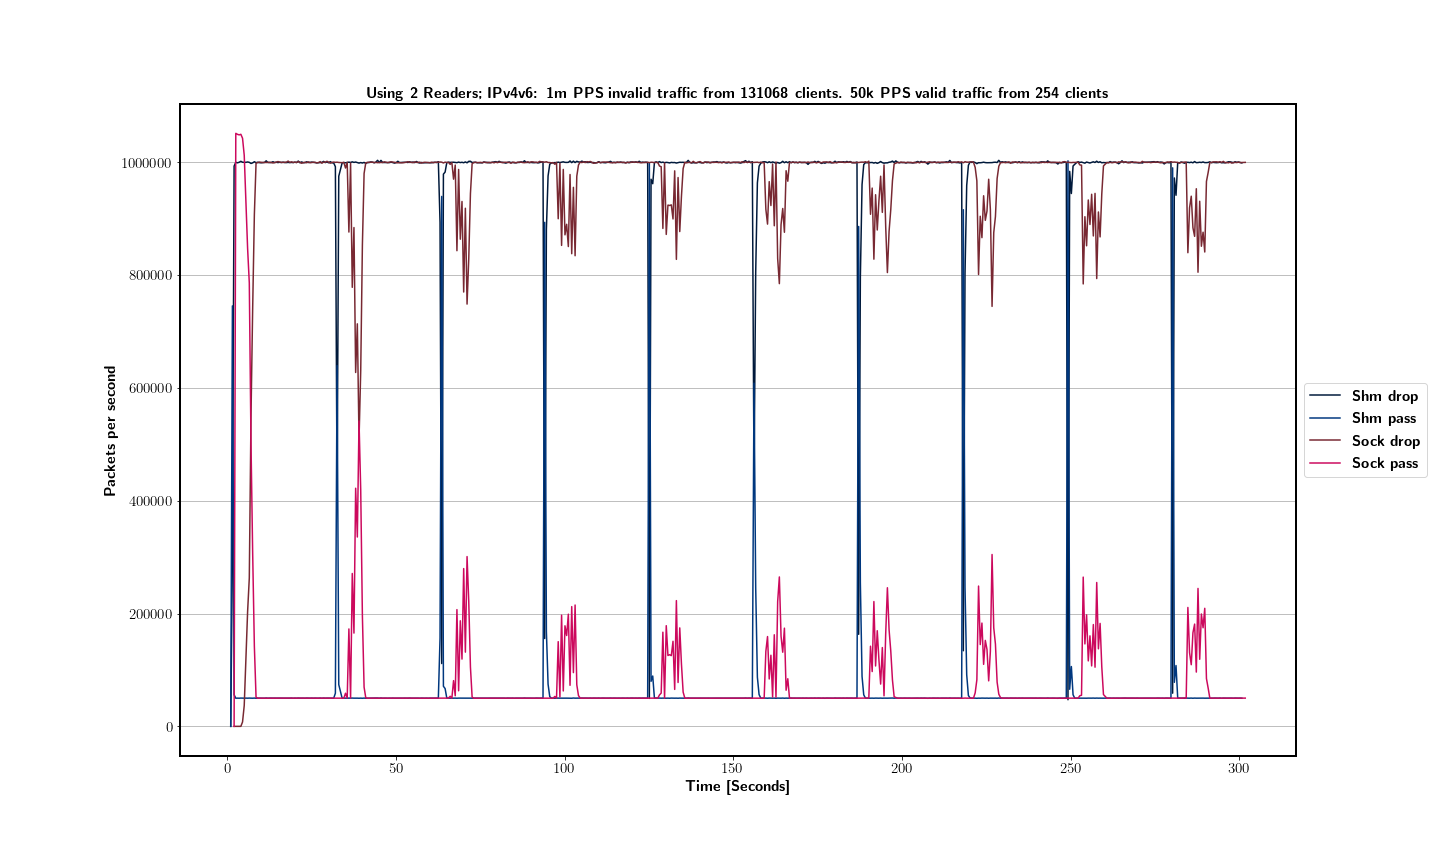
\includegraphics[width=1.2\textwidth]{images/IPv4v6_1m_2ndReader_1.png}}
	\end{tabular}
	\begin{tabular}{llll}
		\toprule
		\textbf{IPC type} & \textbf{XDP\_DROP [$10^7$]} & \textbf{XDP\_PASS [$10^6$]} & \textbf{Relative drop [\%]} \\ \midrule 
		Shm & 29,53 & 19,75 & 99,72283593 \\
        Sock & 28,91 & 25,94 & 97,6334018 \\
	\bottomrule
	\end{tabular}
    \begin{tabular}{llll}
		\toprule
		\textbf{IPC type} & \textbf{Packets received by udp\_server [$10^6$]} & \textbf{Log messages [$10^5$]} & \textbf{CPU [seconds]} \\ \midrule 
		Shm & 19,48 & 44,91 & 17.76 \\
        Sock & 18,29 & 41,47 & 80.82 \\
	\bottomrule
	\end{tabular}
	\caption[Simplefail2ban with 2nd Reader, IPv4v6, 1m \ac{PPS}, 131068 malicious clients]{Total packets sent: 315m. Best-case drop rate: 98,68932\%}
	\label{fig:data:ipv4v6:1m:131068:2nd}
\end{figure}

Figure \ref{fig:data:ipv4v6:20m:131068:2nd} shows data measured with 20m invalid \ac{PPS}.
The socket \ac{IPC} type struggles to supply both the \ac{IPS} and the second reader with \texttt{log messages}, having logged less data than the shared memory \ac{IPC} type.
The graph also displays this inability to keep up with incoming traffic during the first two ban cycles.
While shared memory was able to fully ban all malicious client in just one 30 second ban cycle, the socket mode is not.
Given enough time, the socket \ac{IPC} type is able to recover and successfully defend against the \ac{DoS} attack.

\begin{figure}[!h]
	\centering
	\scriptsize
	\begin{tabular}{c}
    	\centerline{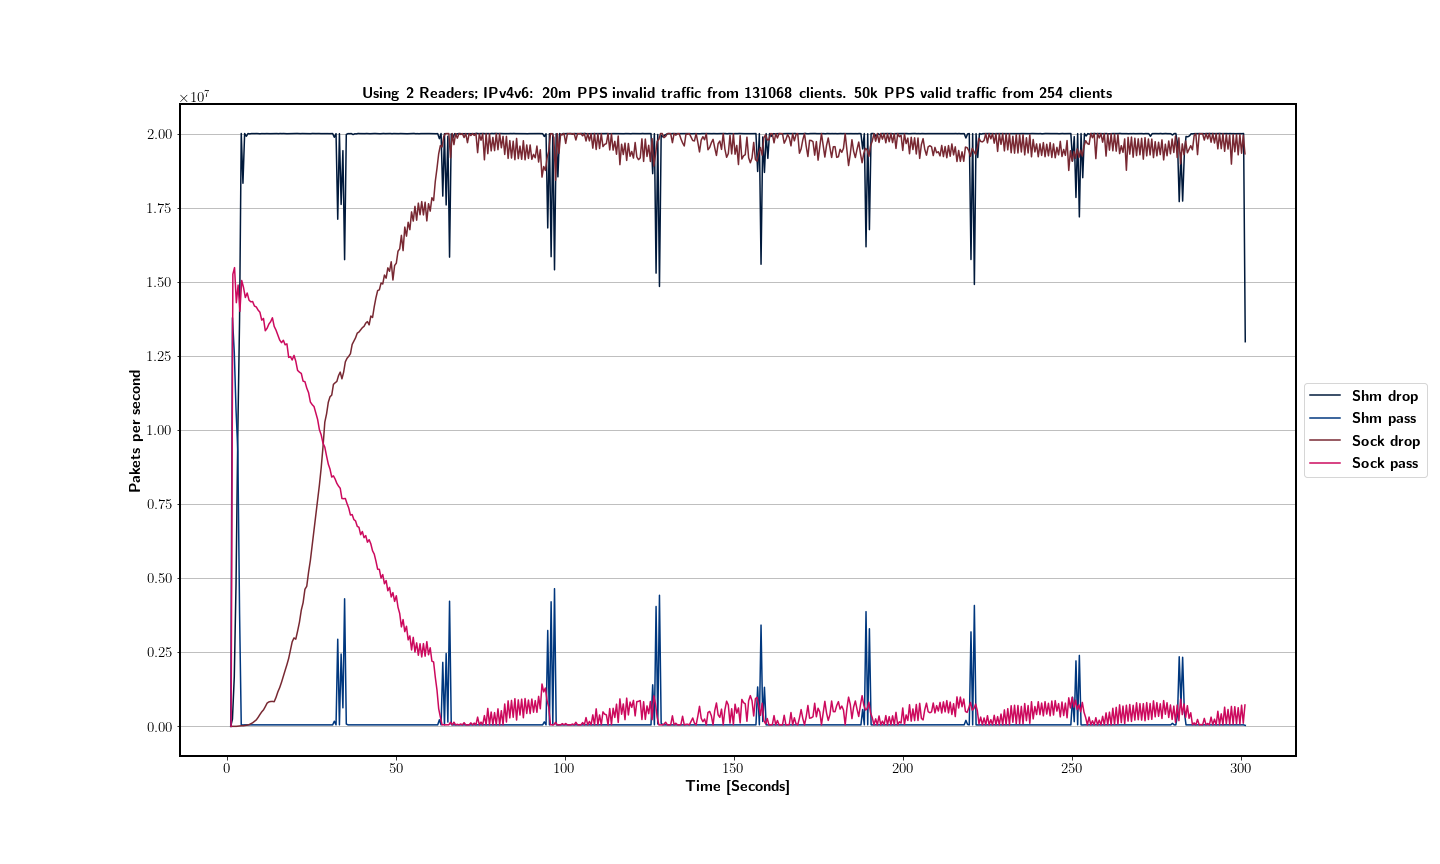
\includegraphics[width=1.2\textwidth]{images/IPv4v6_20m_2ndReader_1.png}}
	\end{tabular}
	\begin{tabular}{llll}
		\toprule
		\textbf{IPC type} & \textbf{XDP\_DROP [$10^8$]} & \textbf{XDP\_PASS [$10^6$]} & \textbf{Relative drop [\%]} \\ \midrule 
		Shm & 59,15 & 79,92 & 98,64873119 \\
        Sock & 52,45 & 624,81 & 87,47139407 \\
	\bottomrule
	\end{tabular}
    \begin{tabular}{llll}
		\toprule
		\textbf{IPC type} & \textbf{Packets received by udp\_server [$10^6$]} & \textbf{Log messages [$10^5$]} & \textbf{CPU [seconds]} \\ \midrule 
		Shm & 24,61 & 101,26 & 49.90 \\
        Sock & 11,32 & 65,01 & 251.49 \\
	\bottomrule
	\end{tabular}
	\caption[Simplefail2ban with 2nd Reader, IPv4v6, 20m \ac{PPS}, 131068 malicious clients]{Total packets sent: 6015m. Best-case drop rate: 99,934466\%}
	\label{fig:data:ipv4v6:20m:131068:2nd}
\end{figure}

That changes in figure \ref{fig:data:ipv4v6:30m:131068:2nd}.
Now, the socket \ac{IPC} type is unable to defend against the \ac{DoS} attack, and the system is overwhelmed - failing to drop all invalid traffic.  
The \texttt{relative drop} falls to approximately 54 percent, the number of messages passed to the kernel rise significantly and the application udp\_server is not able to handle the influx of incoming data.
Fewer log messages are sent to all readers and the \ac{CPU} time falls, likely due to the system not having any resources left for user space applications.
Meanwhile, the shared memory \ac{IPC} type performs just as well as in figure \ref{fig:data:ipv4v6:30m:131068}, when no second reader was attached to the \ac{IPC} architecture.

A difference of this scale was not initially expected.
However, increased performance of the shared memory \ac{IPC} type was attributed to the overwrite feature.
Enabling this feature meant that slower reader processes were ignored if they slowed down any writers.
The socket \ac{IPC} type cannot abandon slow readers, it has to wait for each reader to receive all data, unlike the shared memory \ac{IPC}.

\begin{figure}[!h]
	\centering
	\scriptsize
	\begin{tabular}{c}
    	\centerline{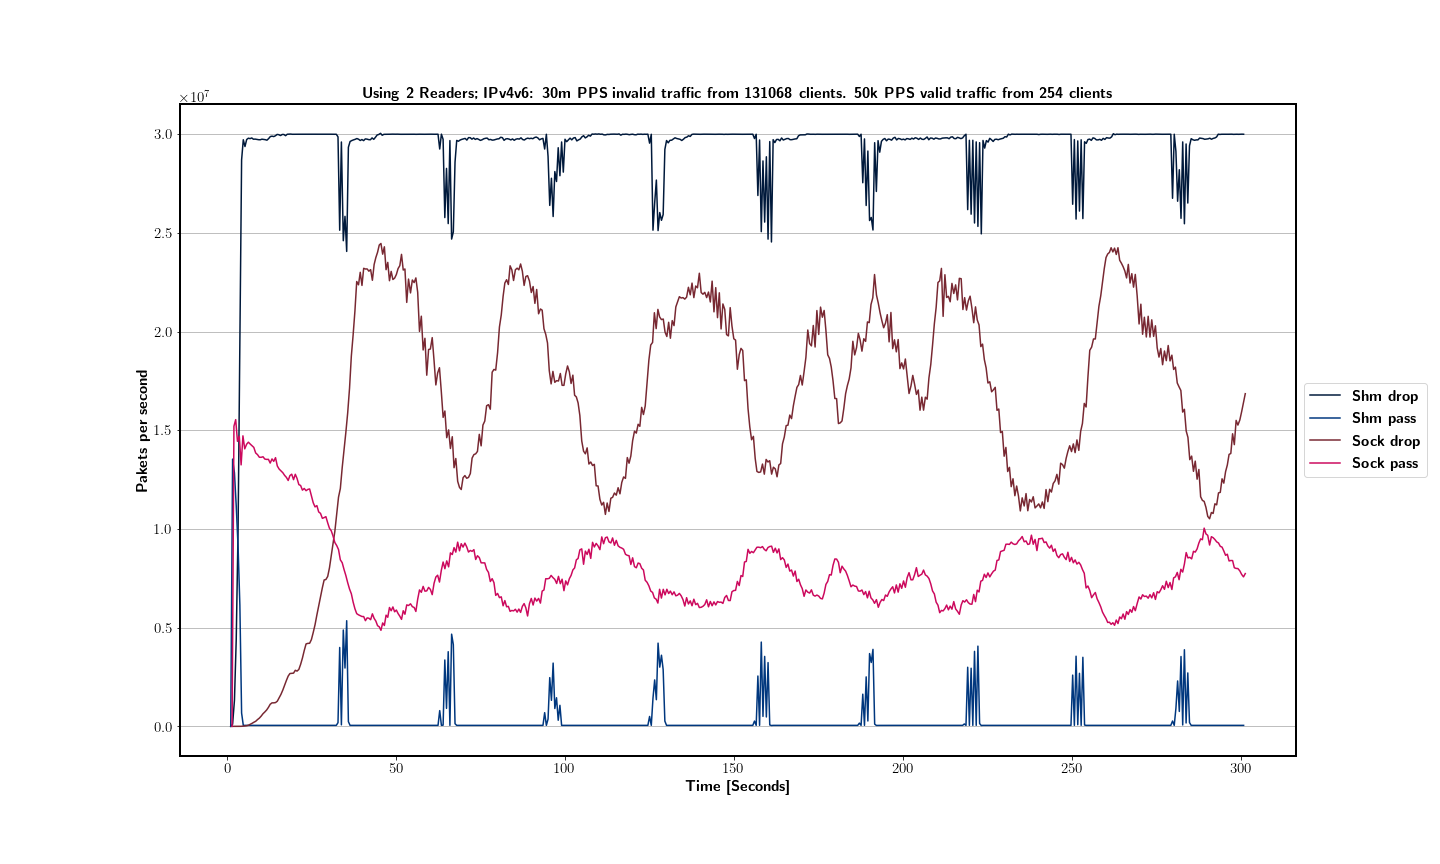
\includegraphics[width=1.2\textwidth]{images/IPv4v6_30m_2ndReader_1.png}}
	\end{tabular}
	\begin{tabular}{llll}
		\toprule
		\textbf{IPC type} & \textbf{XDP\_DROP [$10^8$]} & \textbf{XDP\_PASS [$10^6$]} & \textbf{Relative drop [\%]} \\ \midrule 
		Shm & 87,83 & 118,74 & 97,63360872 \\
        Sock & 48,80 & 2385,53 & 54,22323337 \\
	\bottomrule
	\end{tabular}
    \begin{tabular}{llll}
		\toprule
		\textbf{IPC type} & \textbf{Packets received by udp\_server [$10^6$]} & \textbf{Log messages [$10^5$]} & \textbf{CPU [seconds]} \\ \midrule 
		Shm & 24,70 & 108,17 & 94.60 \\
        Sock & 3,10 & 30,04 & 31.91 \\
	\bottomrule
	\end{tabular}
	\caption[Simplefail2ban with 2nd Reader, IPv4v6, 30m \ac{PPS}, 131068 malicious clients]{Total packets sent: 9015m. Best-case drop rate: 99,95631067\%}
	\label{fig:data:ipv4v6:30m:131068:2nd}
\end{figure}

Another experiment was conducted to confirm the link between enabling the overwrite feature and the increased performance of the shared memory \ac{IPC} type:
The shared memory \ac{IPC} type is used without having the overwrite feature enabled.
Expectations were, that having to wait for all reader processes to receive data would result in a performance decrease.
This measurement is displayed in figure \ref{fig:data:ipv4v6:30m:131068:2nd:NoOverwrite}.

No such decrease in performance was measured whatsoever.
The only logical conclusion is, that the shared memory \ac{IPC} type manages to supply multiple readers with faster data transfer than is required for even 30m incoming invalid \ac{PPS}.
The overwrite feature was not needed and had no real impact on performance.
Increased latency when using the socket \ac{IPC} type likely culminated to such a degree that supplying multiple readers with data was not feasible.

\begin{figure}[!h]
	\centering
	\scriptsize
	%\begin{tabular}{c}
    %	\centerline{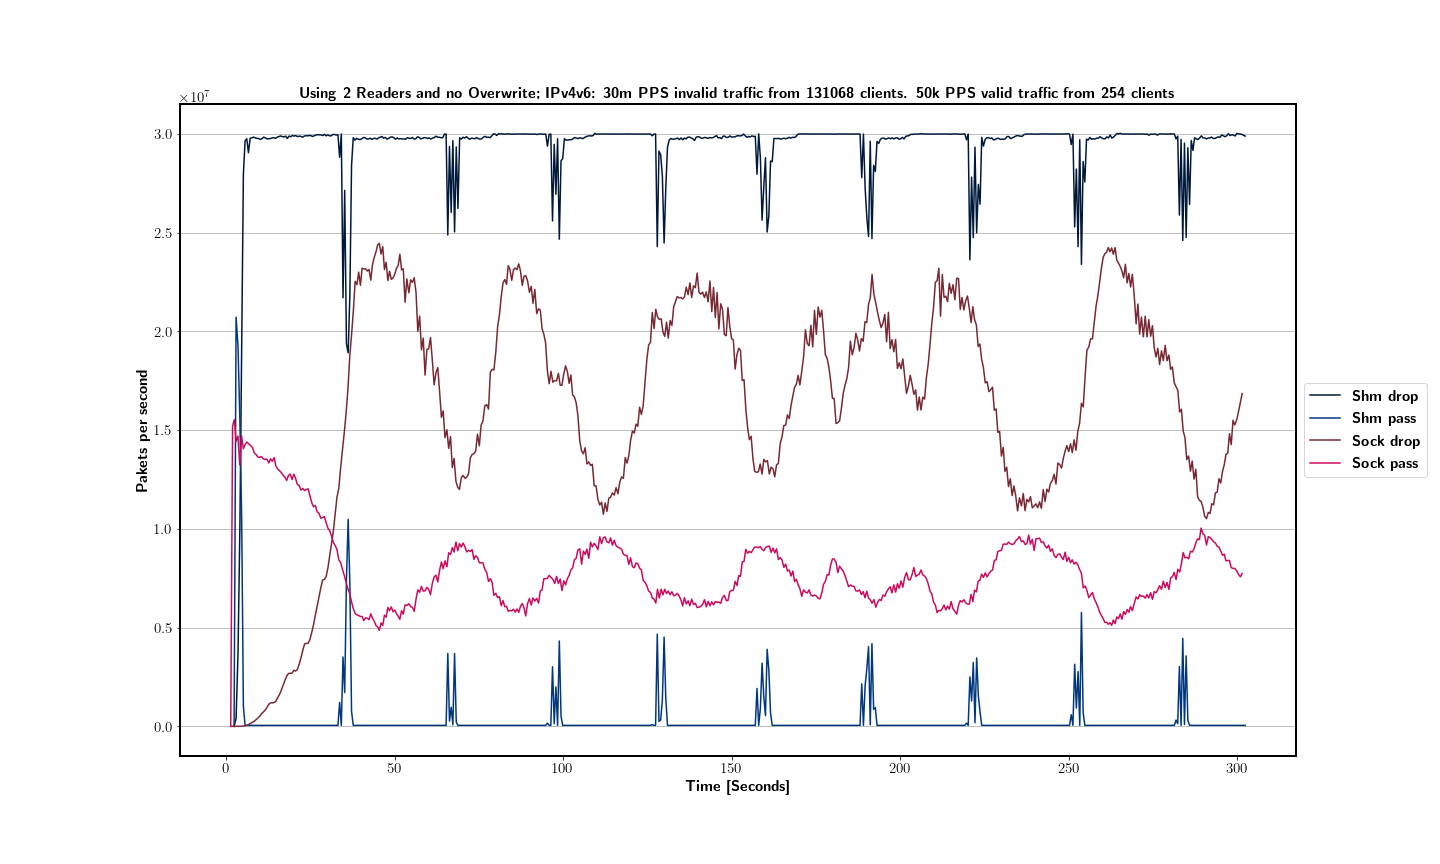
\includegraphics[width=1.2\textwidth]{images/IPv4v6_30m_2ndReaderNoOverwrite_1.png}}
	%\end{tabular}
	\begin{tabular}{llll}
		\toprule
		\textbf{IPC type} & \textbf{XDP\_DROP [$10^8$]} & \textbf{XDP\_PASS [$10^6$]} & \textbf{Relative drop [\%]} \\ \midrule 
		Shm & 87,99 & 125,56 & 97,81321365 \\
        Sock & 48,80 & 2385,53 & 54,22323337 \\
	\bottomrule
	\end{tabular}
    \begin{tabular}{llll}
		\toprule
		\textbf{IPC type} & \textbf{Packets received by udp\_server [$10^6$]} & \textbf{Log messages [$10^5$]} & \textbf{CPU [seconds]} \\ \midrule 
		Shm & 24,95 & 108,43 & 99.47 \\
        Sock & 3,10 & 30,04 & 31.91 \\
	\bottomrule
	\end{tabular}
	\caption[Simplefail2ban with 2nd Reader, IPv4v6, 30m \ac{PPS}, 131068 malicious clients]{Total packets sent: 9015m. Best-case drop rate: 99,95631067\%}
	\label{fig:data:ipv4v6:30m:131068:2nd:NoOverwrite}
\end{figure}
    
    \acresetall % reset acronym counter
    %
% chapter6.tex
%

\chapter{Conclusion \& Outlook}
In this thesis, the previously developed light-weight \ac{IPS} Simplefail2ban and its selection of \ac{IPC} was expanded to include unix domain sockets.
With it being the first kernel-based \ac{IPC} available, thorough measurements were conducted to evaluate its performance to the already implemented shared memory and file-base \ac{IPC} modes.
Expectations were that unix domain sockets would not outperform shared memory, because of a constant need for context-switches between kernel- and userspace.
This initial hypothesis turned out to be true.
The socket \ac{IPC} type was beat in all analyzed metrics (number of unwanted requests dropped, number of log messages sent and \ac{CPU} time) by the shared memory mode of Simplefail2ban.
However, performance of the unix domain socket mode was still well up to the task.
It remained competitive in experiments utilizing only one process to receive data, performing only around 2 percent worse than its shared memory counterpart.
During less intense traffic flow, this small disadvantage in performance shrunk even further.
Data indicates that latency in the socket \ac{IPC} type was at least on par with the shared memory mode.
Rather, a lack of bandwidth and increased drain on system resources are the main causes identified for the observed decrease in performance.
Conversely, unix domain socket did consistently outperform the file-based \ac{IPC}, albeit by a small fraction: regularly being less than one percentage point in relative drop rate.
Overall, the socket \ac{IPC} type was always able to block over 95,5 percent (and 98,5 percent on average) of all incoming traffic, therefore defending against \ac{DoS} attacks successfully.

While never being an explicitly desired feature, the socket \ac{IPC} type does provide the option to attach, up to a pre-defined maximum, and detach a varying number of both writer and reader processes during runtime.
In contrast, the shared memory \ac{IPC} only provides the option to attach multiple reader processes.
This allows for, in theory, flexible reusing of the socket \ac{IPC} architecture for other applications.
Regrettably however, usage of unix domain sockets in scenarios with multiple reader processes is not recommended due to a lack of bandwidth, resulting in the socket \ac{IPC} performing significantly worse than the shared memory \ac{IPC}.
At a rate of 20m invalid \ac{PPS}, defending against a \ac{DoS} attack in a single ban cycle was unfeasible when employing unix domain sockets.
Yet, after multiple ban cycles, Simplefail2ban was able to recover and repel the incoming \ac{DoS} attack.
With 30m invalid \ac{PPS}, a recovery became impossible.
The shared memory \ac{IPC} type was able to keep its performance up even when supplying a second reader process, and disabling the overwrite feature.

Potential improvements of the socket \ac{IPC} should focus on increasing the bandwidth.
This makes it possible to react more efficiently and effectively in the event of a sudden influx of messages, primarily occurring at the beginning of a ban cycle or \ac{DoS} attack.

Overall, this thesis proved that the kernel-based unix domain sockets remain a viable option as \ac{IPC} coming reasonably close to, yet unable to surpass the higher performance of the shared memory \ac{IPC} type.
Continued development could focus on the possibility of scaling the socket \ac{IPC} beyond the local system by employing internet sockets.
Providing an improved high-level \ac{API} for easier integrability with established real-world applications, such as syslog or journald, is also worthwhile investigating.
    
    %
% $Id: outro.tex 2771 2008-10-15 16:29:47Z sliske $
%
\addtocontents{toc}{\protect\newpage}
% start the appendix (changes section numbering, and others)
\appendix
% use different page style
\pagestyle{appendixstyle}
%reset acronym counter
% \acresetall % really? (by stefan)

%list of figures
%

\listoffigures
%\cleardoublepage

%
% list of tables
%

\listoftables
%\cleardoublepage

%
% list of algorithms
%

\listofalgorithms
%\cleardoublepage

%
% list of abbreviations
%

\iflanguage{ngerman}
{
\chapter{Abkürzungsverzeichnis}
}{
\chapter{Abbreviations}
}
\begin{acronym}[skbufflonglon]
\acro{API}{Application Programming Interface}
\acro{AMQP}{Advanced Message Queue Protocol}
\acro{ARM}{Advanced \acs{RISC} Machines}
\acro{BCC}{BPF Compiler Collection}
\acro{BIND}{Berkeley Internet Name Domain Server}
 \acro{BPF}{Berkeley Packet Filter}
 \acro{BPF CORE}{BPF Compile Once Run Everywhere}
 \acro{BTF}{BPF Type Format}
 \acro{cBPF}{classical Berkeley Packet Filter}
 \acro{CPU}{Central Processing Unit}
 \acro{DNS}{Domain Name System}
 \acro{DUT}{Device under Test}
 \acro{DDIO}{Direct Data Input Output}
 \acro{DoS}{Denial of Service}
 \acro{DDoS}{Distributed Denial of Service}
 \acro{DMA}{Direct Memory Access}
 \acro{DPDK}{Data Plane Development Kit}
 \acro{eBPF}{extended Berkeley Packet Filter}
 \acro{ESP}{Encapsulating Security Payload}
 \acro{FIFO}{First in First out}
 \acro{HIDS}{Host-based Intrusion Detection System}
 \acro{HTTP}{Hypertext Transfer Protocol}
 \acro{IANA}{Internet Assigned Numbers Authority}
 \acro{IDS}{Intrusion Detection System}
 \acro{IEEE}{Institute of Electrical and Electronics Engineers}
 \acro{IP}{Internet Protocol}
 \acro{IPC}{Inter-Process Communication}
 \acro{IPS}{Intrusion Prevention System}
 \acro{IPsec}{\acs{IP} Security}
 \acro{IPv4}{Internet Protocol Version 4}
 \acro{IPv6}{Internet Protocol Version 6}
 \acro{IO}{Input / Output}
 \acro{ISP}{Internet Service Provider}
 \acro{JIT}{Just in Time}
 \acro{LLVM}{Low Level Virtual Machine}
 \acro{MAC}{Media Control Access}
 \acro{MPPS}{Million Packets Per Second}
 \acro{MTU}{Maximum Transfer Unit}
 \acro{NAPI}{New \acs{API}}
 \acro{API}{Application Programming Interface}
 \acro{NAT}{Network Address Translation}
 \acro{NIC}{Network Interface Card}
 \acro{NIDS}{Network-based Intrusion Detection System}
 \acro{NSD}{Name Server Daemon}
 \acro{pcap}{Packet Capture}
 \acro{OS}{Operating System}
 \acro{OSI}{Open Systems Interconnection}
 \acro{PCI}{Peripheral Component Interconnect}
 \acro{PoC}{Proof of Concept}
 \acro{PPS}{Packets per Second}
 \acro{RAM}{Random Access Memory}
 \acro{regex}{regular expression}
 \acro{RIPE}{Réseaux IP Européens (European \ac{IP} Networks)}
 \acro{RISC}{Reduced Instruction Set Computer}
 \acro{RFC}{Request for Comments}
 \acro{Regex}{Regular Expression}
 \acro{skbuff}[\texttt{sk\textunderscore buff}]{Socket Buffer}
 \acro{SSH}{Secure Shell}
 \acro{SIEM}{Security Information and Event Management}
 \acro{tc}[\texttt{tc}]{Traffic Control}
 \acro{TCP}{Transmission Control Protocol}
 \acro{TLS}{Transport Layer Security}
 \acro{UDP}{User Datagram Protocol}
 \acro{VM}{Virtual Machine}
 \acro{VLAN}{Virtual Local Area Network}
 \acro{XDP}{eXpress Data Path}
 \acro{RAM}{Random Access Memory}

 \acrodefplural{OS}[OS's]{Operating Systems}
 \acrodefplural{IPS}[IPS]{Intrusion Detection Systems}
 \acrodefplural{HIDS}[HIDS]{Host-based Intrusion Detection Systems}
 \acrodefplural{NIDS}[NIDS]{Network-based Intrusion Detection Systems}
 \acrodefplural{API}[APIs]{Application Programming Interfaces}


\end{acronym}
%\begingroup
%\let\clearpage\relax
\chapter{Source Files}
For the sake of not having to chop down a forest to print this thesis, no full source files will be appended.
The source code is available in a git repository at: \href{https://gitup.uni-potsdam.de/raatschen/bachelorarbeit}{https://gitup.uni-potsdam.de/raatschen/bachelorarbeit}.
Access can be requested through me, or the second supervisor Max Schrötter.
%\endgroup

\chapter{Measurements}


\begin{figure}[h!p]
	
	\centering
	\scriptsize
	\begin{tabular}{c}
    	\centerline{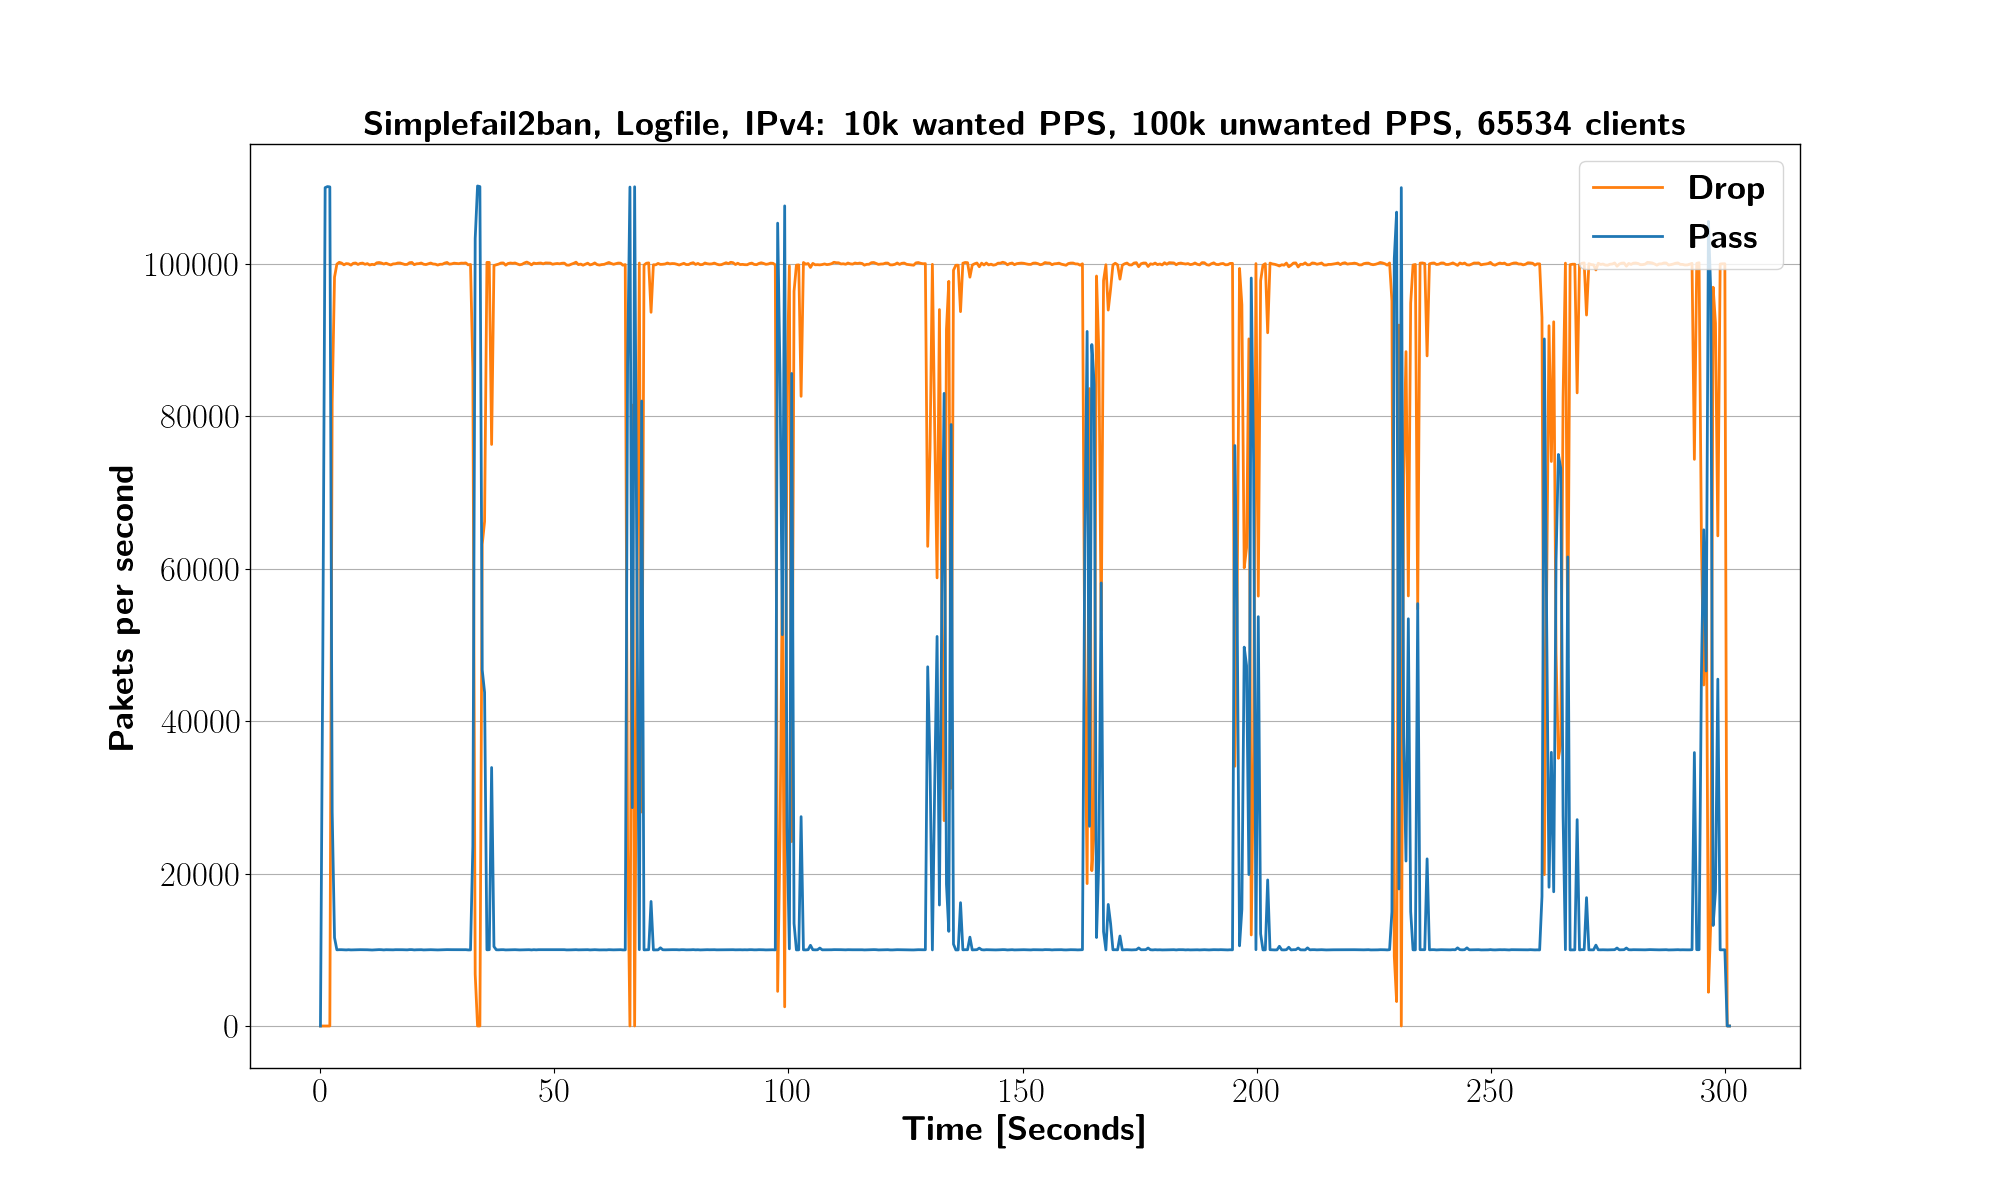
\includegraphics[width=1.2\textwidth]{images/simplefail2ban_disk_ipv4_v10k_iv100k_c65534.png}}
	\end{tabular}
	\begin{tabular}{lllll}
		\toprule
		\textbf{Total packets [$10^6$]} & \textbf{Packets dropped [$10^6$]} & \textbf{Relative drop [\%]} & \textbf{Log messages [$10^6$]} & \textbf{CPU [seconds]} \\ \midrule 
		33 & 27.93 & 99.59 & 2.07 & 10.51 \\
		\bottomrule
	\end{tabular}
	\caption[Simplefail2ban, Logfile IPv4, 100k \ac{PPS}]{Simplefail2ban Logfile \ac{IPv4}, 10 thousand unwanted \ac{PPS}, 100 thousand wanted \ac{PPS}, 65534 clients.}
	\label{fig:simplefail2ban:disk:ip4:100k}
\end{figure}

\begin{figure}[h!]
	\centering
	\scriptsize
	\begin{tabular}{c}
    	\centerline{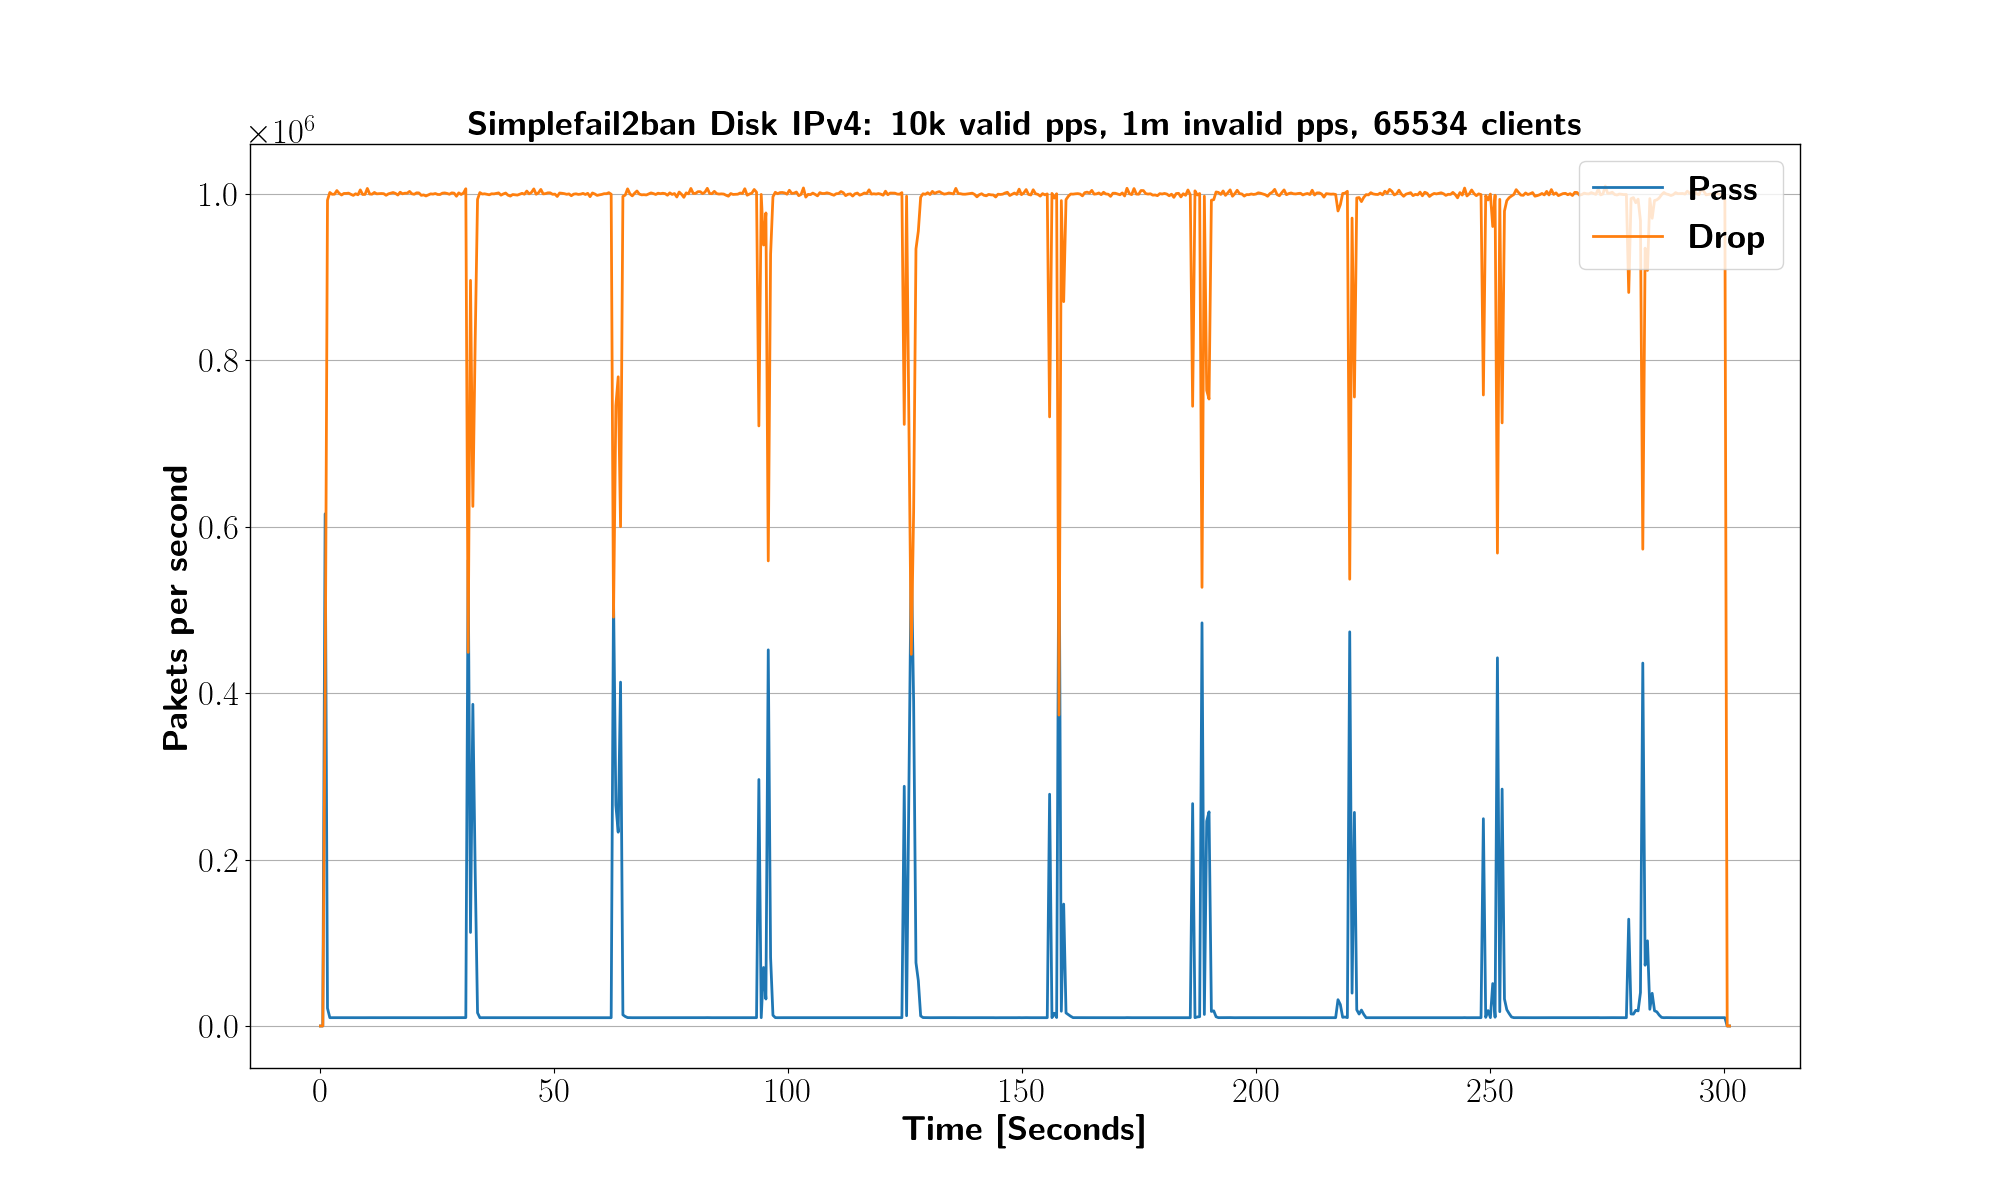
\includegraphics[width=1.2\textwidth]{images/simplefail2ban_disk_ipv4_v10k_iv1m_c65534.png}}
    \end{tabular}
	\begin{tabular}{lllll}
		\toprule
		\textbf{Total packets [$10^6$]} & \textbf{Packets dropped [$10^6$]} & \textbf{Relative drop [\%]} & \textbf{Log messages [$10^6$]} & \textbf{CPU [seconds]} \\ \midrule 
		303 & 294.43 & 98.79 & 4.7 & 14.99 \\
		\bottomrule
	\end{tabular}
	\caption[Simplefail2ban, Logfile IPv4, 1m \ac{PPS}]{Simplefail2ban Logfile \ac{IPv4}, 10 thousand unwanted \ac{PPS}, 1 million wanted \ac{PPS}, 65534 clients.}
	\label{fig:simplefail2ban:disk:ip4:1m}
\end{figure}

\begin{figure}[h!]
	\centering
	\scriptsize
	\begin{tabular}{c}
    	\centerline{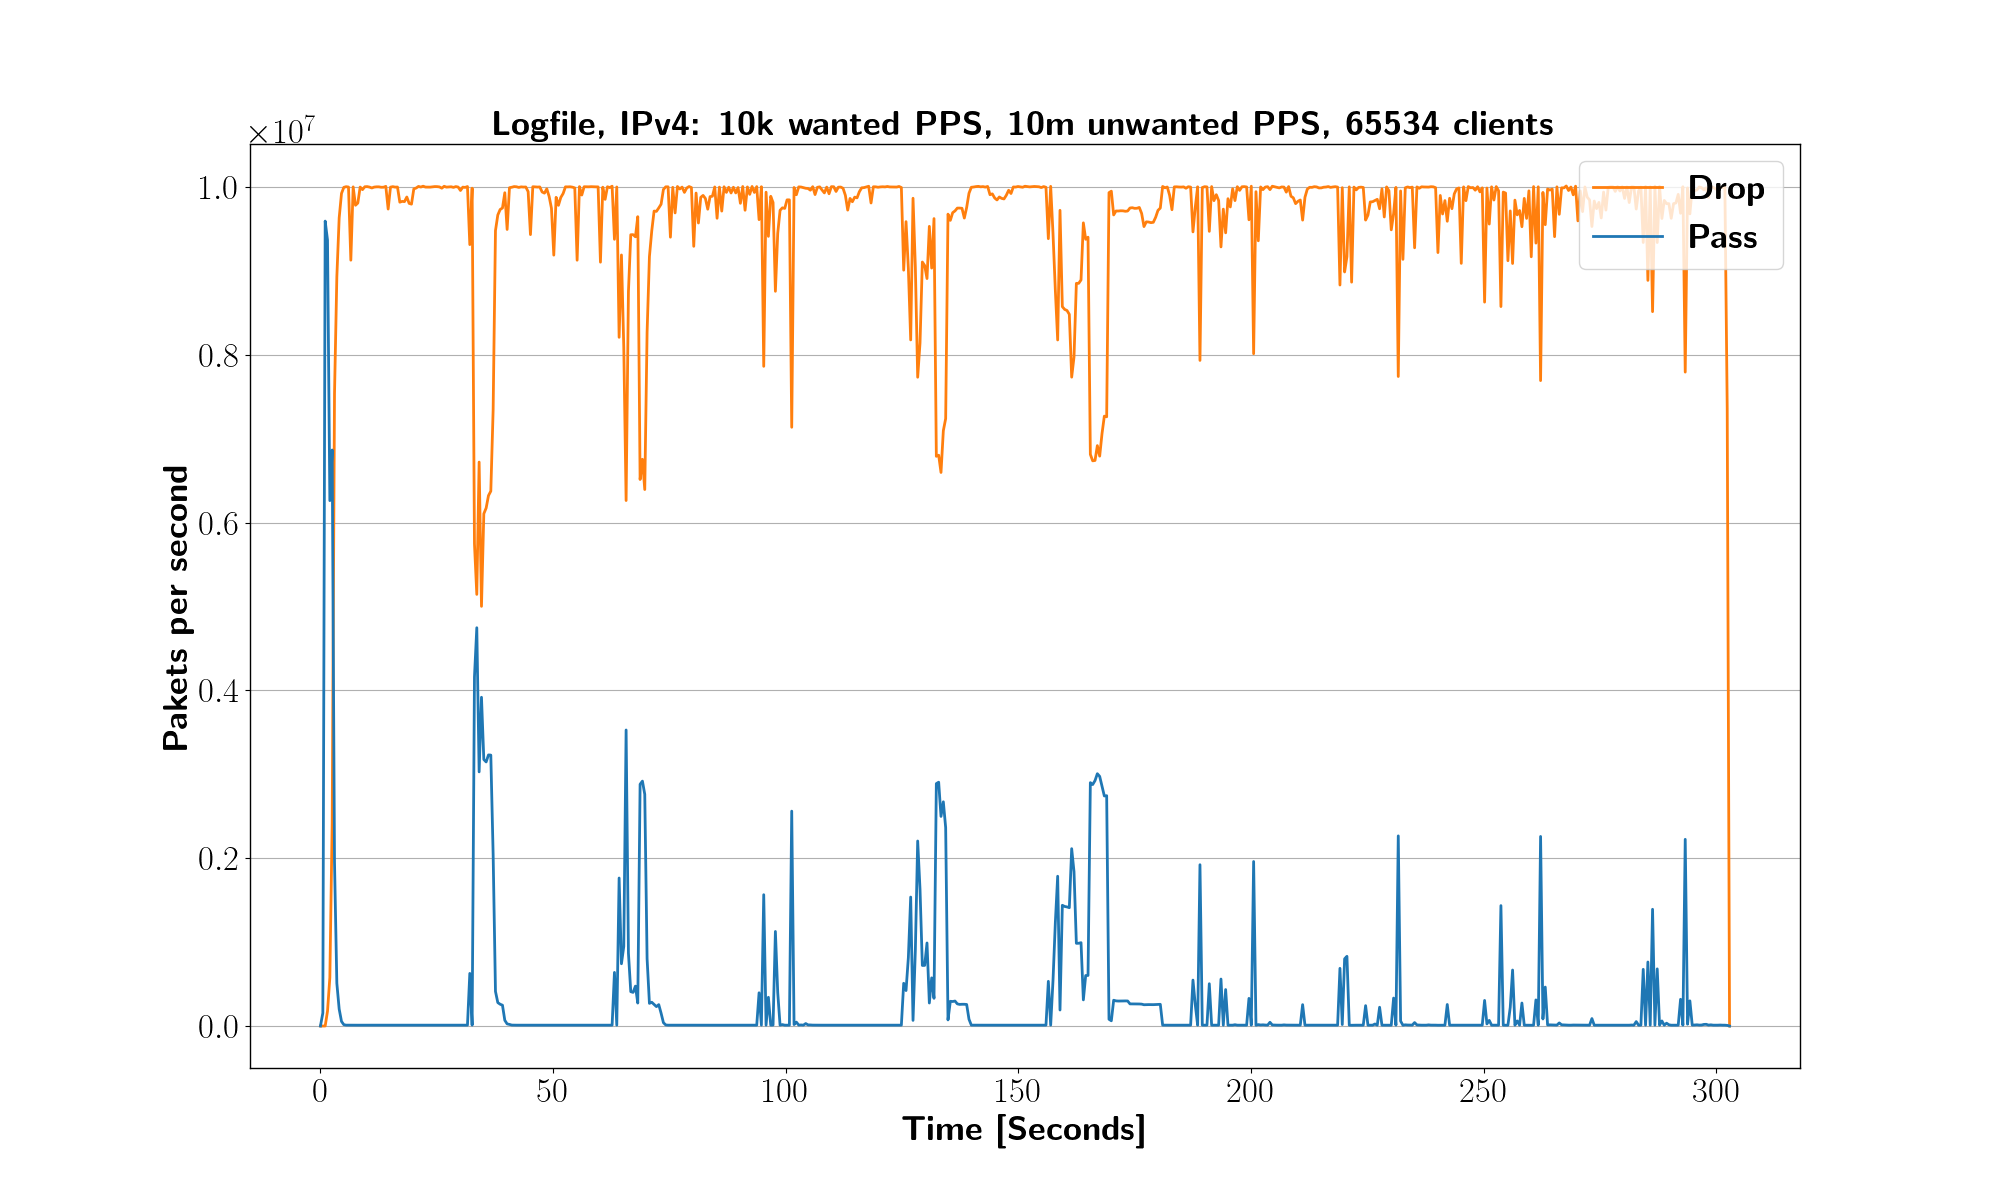
\includegraphics[width=1.2\textwidth]{images/simplefail2ban_disk_ipv4_v10k_iv10m_c65534.png}}
	\end{tabular}
	\begin{tabular}{lllll}
		\toprule
		\textbf{Total packets [$10^6$]} & \textbf{Packets dropped [$10^6$]} & \textbf{Relative drop [\%]} & \textbf{Log messages [$10^6$]} & \textbf{CPU [seconds]} \\ \midrule 
		2986.89 & 2884.14 & 96.72 & 34.39 & 83.72 \\
		\bottomrule
	\end{tabular}
	\caption[Simplefail2ban, Logfile IPv4, 10m \ac{PPS}]{Simplefail2ban Logfile \ac{IPv4}, 10 thousand unwanted \ac{PPS}, 10 million wanted \ac{PPS}, 65534 clients.}
	\label{fig:simplefail2ban:disk:ip4:10m}
\end{figure}

\begin{figure}[!h]
	\centering
	\scriptsize
	\begin{tabular}{c}
    	\centerline{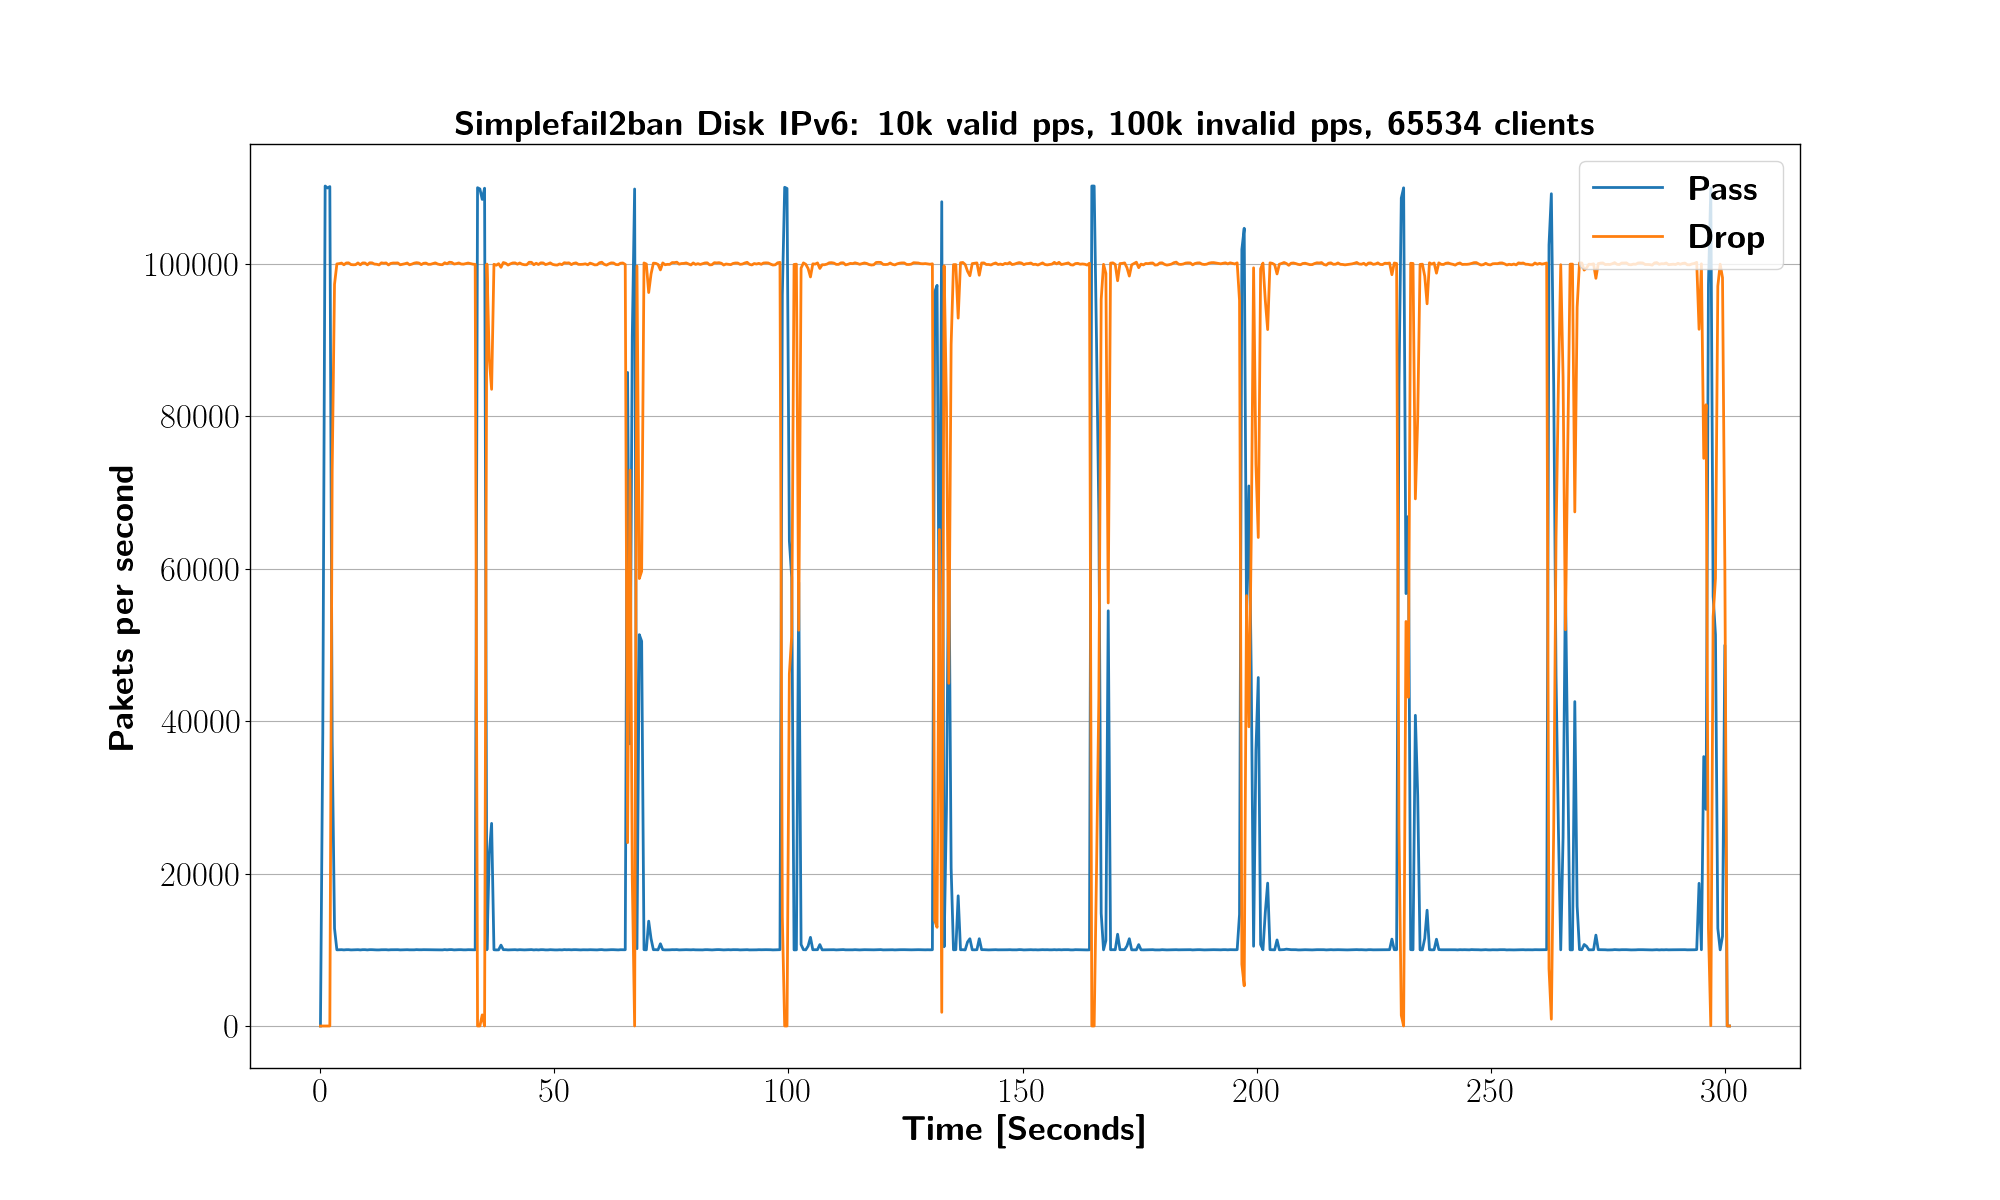
\includegraphics[width=1.2\textwidth]{images/simplefail2ban_disk_ipv6_v10k_iv100k_c65534.png}}
	\end{tabular}
	\begin{tabular}{lllll}
		\toprule
		\textbf{Total packets [$10^6$]} & \textbf{Packets dropped [$10^6$]} & \textbf{Relative drop [\%]} & \textbf{Log messages [$10^6$]} & \textbf{CPU [seconds]} \\ \midrule 
		33 & 27.96 & 99.67 & 2.04 & 11.75 \\
		\bottomrule
	\end{tabular}
	\caption[Simplefail2ban, Logfile IPv6, 100k \ac{PPS}]{Simplefail2ban Logfile \ac{IPv6}, 10 thousand wanted \ac{PPS}, 100 thousand unwanted \ac{PPS}, 65534 clients.}
	\label{fig:simplefail2ban:disk:ip6:100k}
\end{figure}

\begin{figure}[!h]
	\centering
	\scriptsize
	\begin{tabular}{c}
    	\centerline{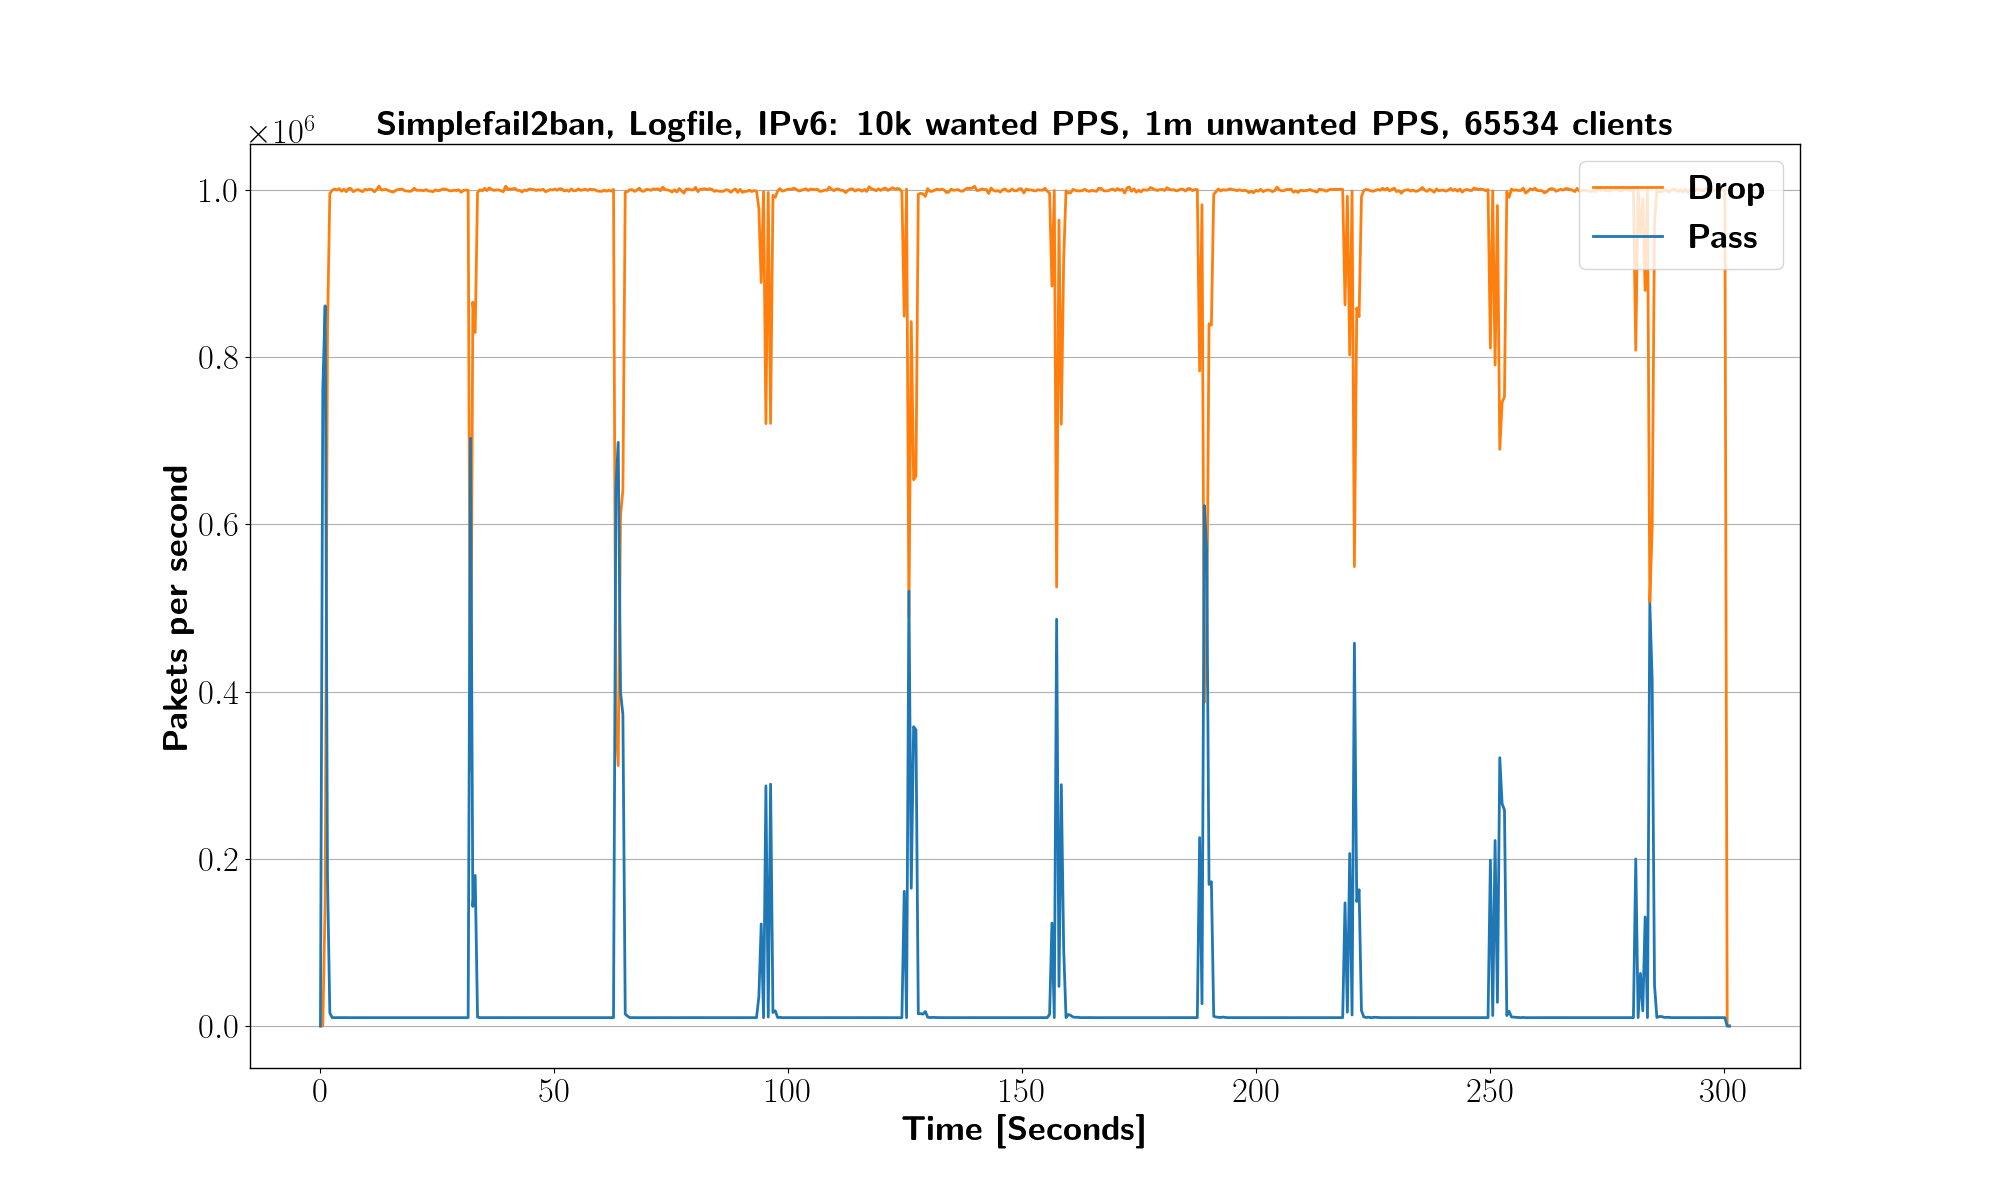
\includegraphics[width=1.2\textwidth]{images/simplefail2ban_disk_ipv6_v10k_iv1m_c65534.png}}
	\end{tabular}
	\begin{tabular}{lllll}
		\toprule
		\textbf{Total packets [$10^6$]} & \textbf{Packets dropped [$10^6$]} & \textbf{Relative drop [\%]} & \textbf{Log messages [$10^6$]} & \textbf{CPU [seconds]} \\ \midrule 
		303 & 293.49 & 98.48 & 5.58 & 21.08 \\
		\bottomrule
	\end{tabular}
	\caption[Simplefail2ban, Logfile IPv6, 1m \ac{PPS}]{Simplefail2ban Logfile \ac{IPv6}, 10 thousand wanted \ac{PPS}, 1 million unwanted \ac{PPS}, 65534 clients.}
	\label{fig:simplefail2ban:disk:ip6:1m}
\end{figure}

\begin{figure}[!h]
	\centering
	\scriptsize
	\begin{tabular}{c}
    	\centerline{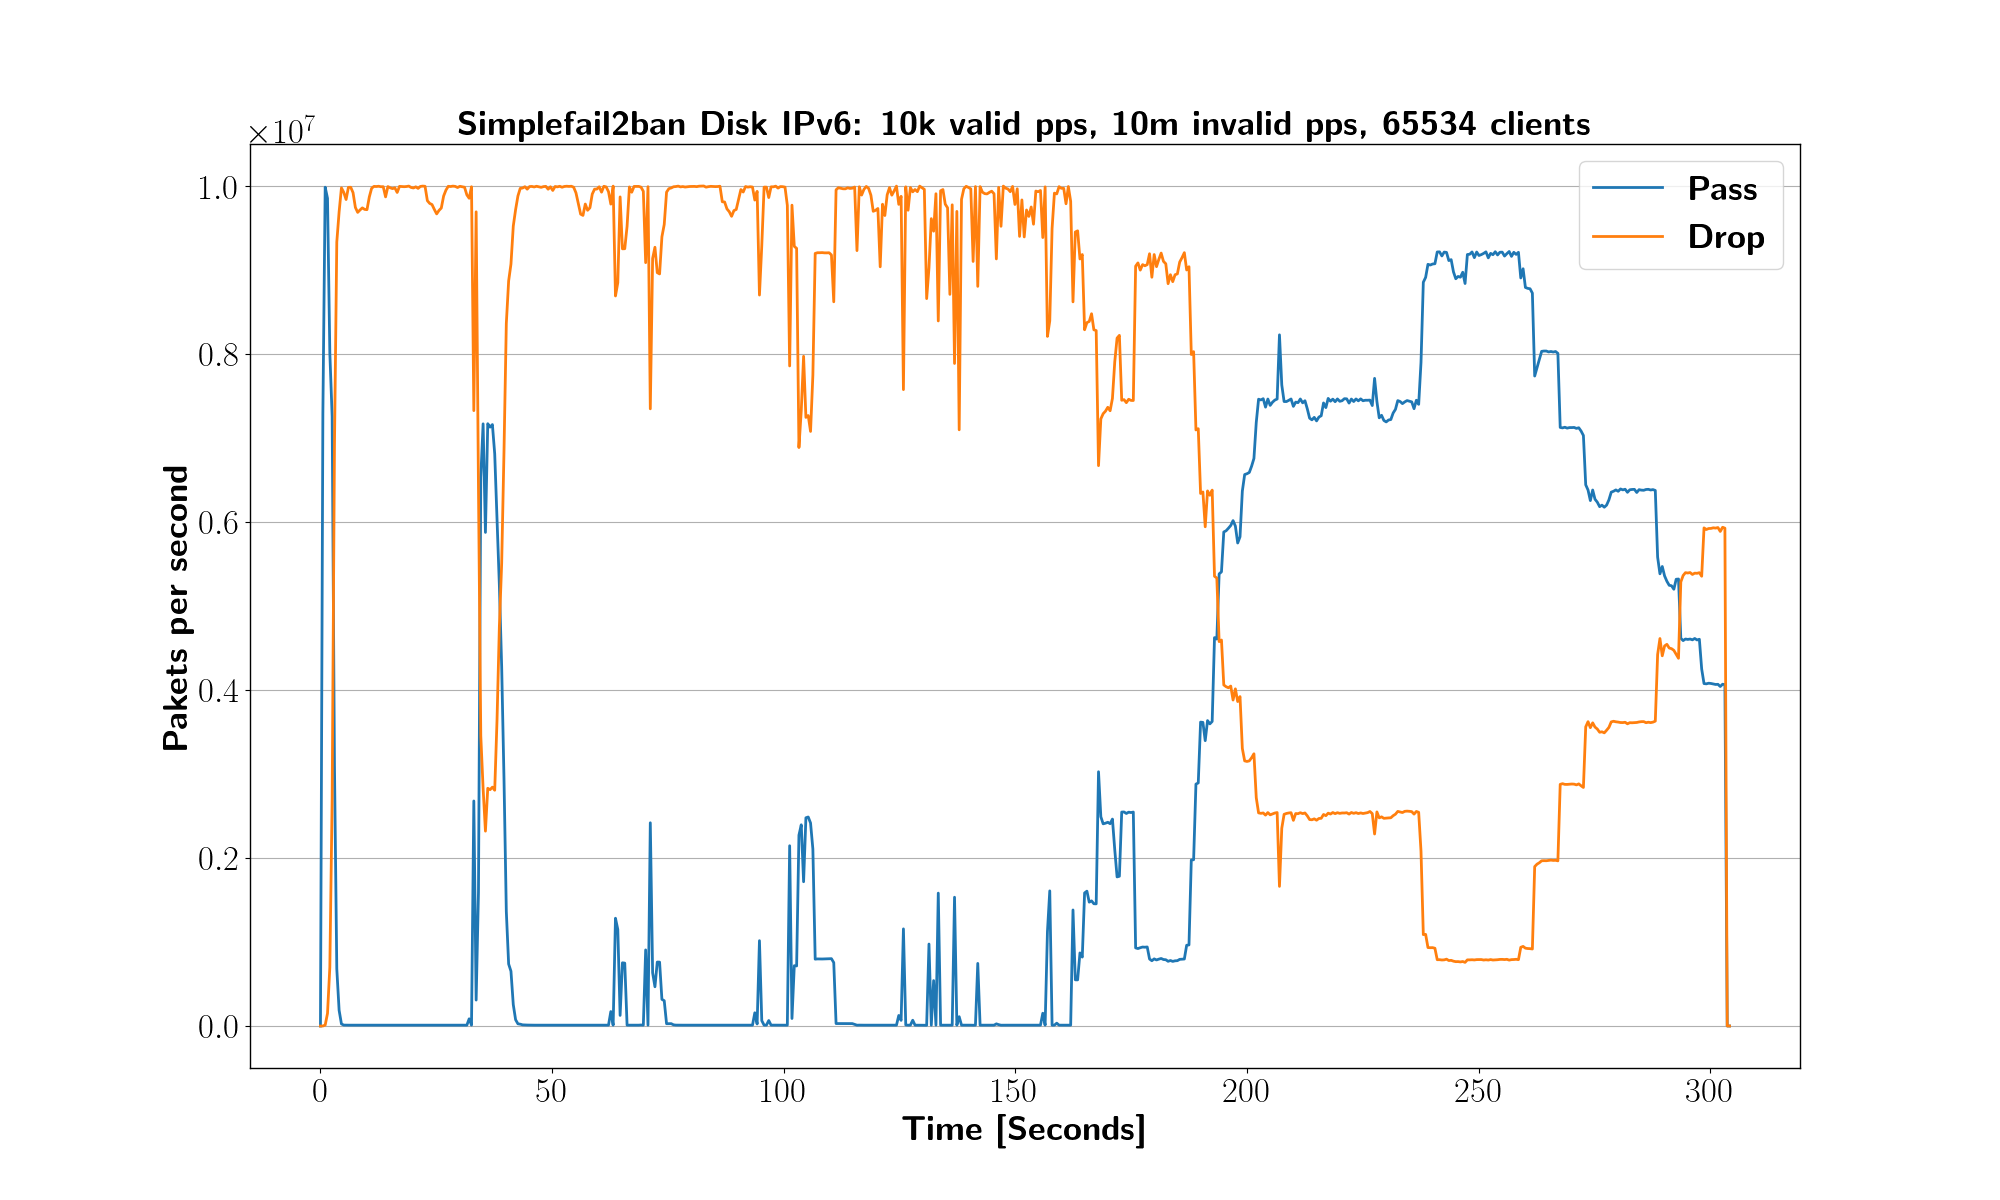
\includegraphics[width=1.2\textwidth]{images/simplefail2ban_disk_ipv6_v10k_iv10m_c65534.png}}
	\end{tabular}
	\begin{tabular}{lllll}
		\toprule
		\textbf{Total packets [$10^6$]} & \textbf{Packets dropped [$10^6$]} & \textbf{Relative drop [\%]} & \textbf{Log messages [$10^6$]} & \textbf{CPU [seconds]} \\ \midrule 
		2992.43 & 2065.28 & 69.13 & 205.4 & 346.73 \\
		\bottomrule
	\end{tabular}
	\caption[Simplefail2ban, Logfile IPv6, 10m \ac{PPS}]{Simplefail2ban Logfile \ac{IPv6}, 10 thousand wanted \ac{PPS}, 10 million unwanted \ac{PPS}, 65534 clients.}
	\label{fig:simplefail2ban:disk:ip6:10m}
\end{figure}


\begin{figure}[!h]
	\centering
	\scriptsize
	\begin{tabular}{c}
    	\centerline{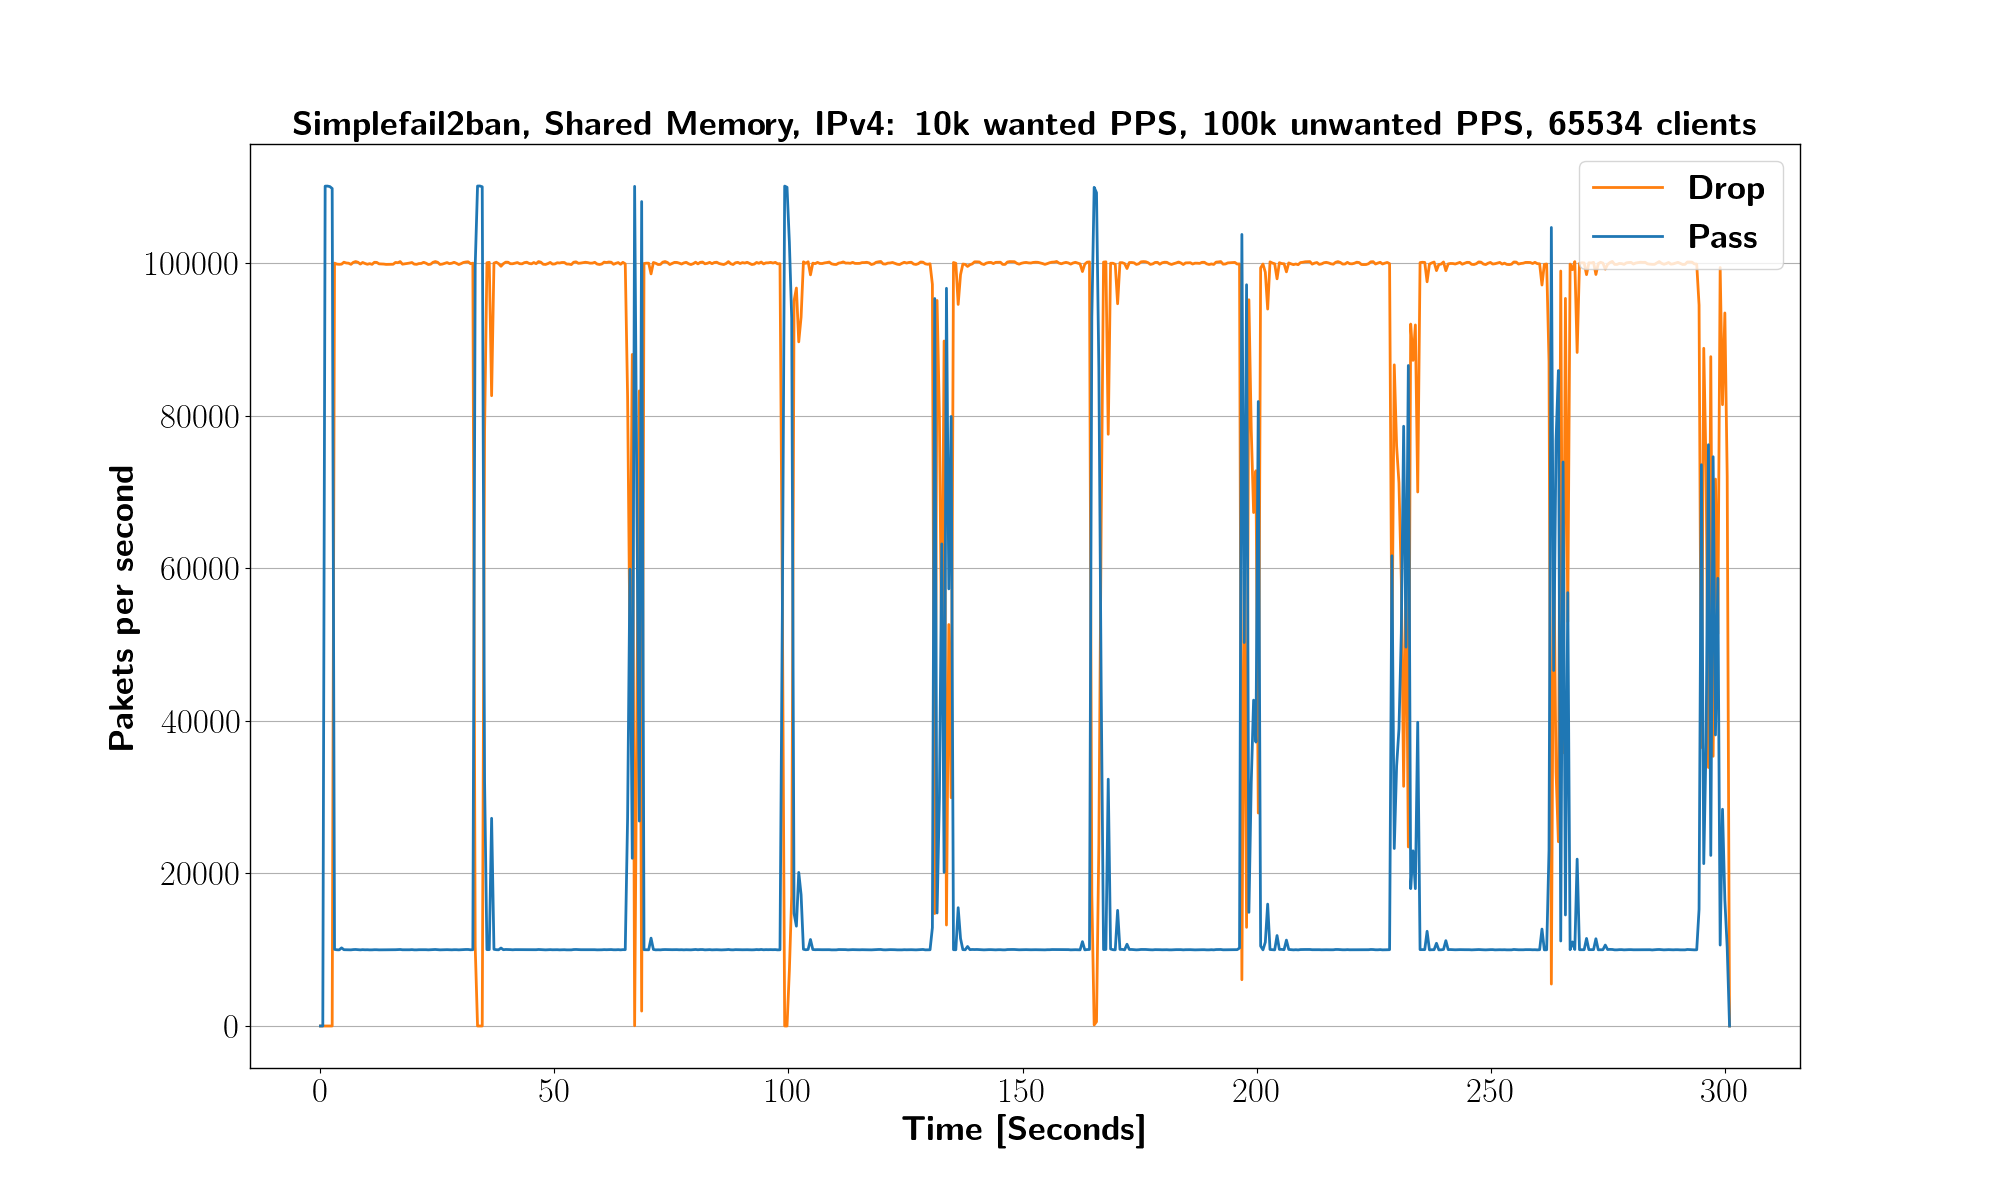
\includegraphics[width=1.2\textwidth]{images/simplefail2ban_shm_ipv4_v10k_iv100k_c65534.png}}
	\end{tabular}
	\begin{tabular}{lllll}
		\toprule
		\textbf{Total packets [$10^6$]} & \textbf{Packets dropped [$10^6$]} & \textbf{Relative drop [\%]} & \textbf{Log messages [$10^6$]} & \textbf{CPU [seconds]} \\ \midrule 
		33 & 27.95 & 99.64 & 2.05 & 13.68 \\
		\bottomrule
	\end{tabular}
	\caption[Simplefail2ban, Shared Memory, IPv4, 100k \ac{PPS}]{Simplefail2ban Shared Memory \ac{IPv4}, 10 thousand wanted \ac{PPS}, 100 thousand unwanted \ac{PPS}, 65534 clients.}
	\label{fig:simplefail2ban:shm:ip4:100k}
\end{figure}

\begin{figure}[!h]
	\centering
	\scriptsize
	\begin{tabular}{c}
    	\centerline{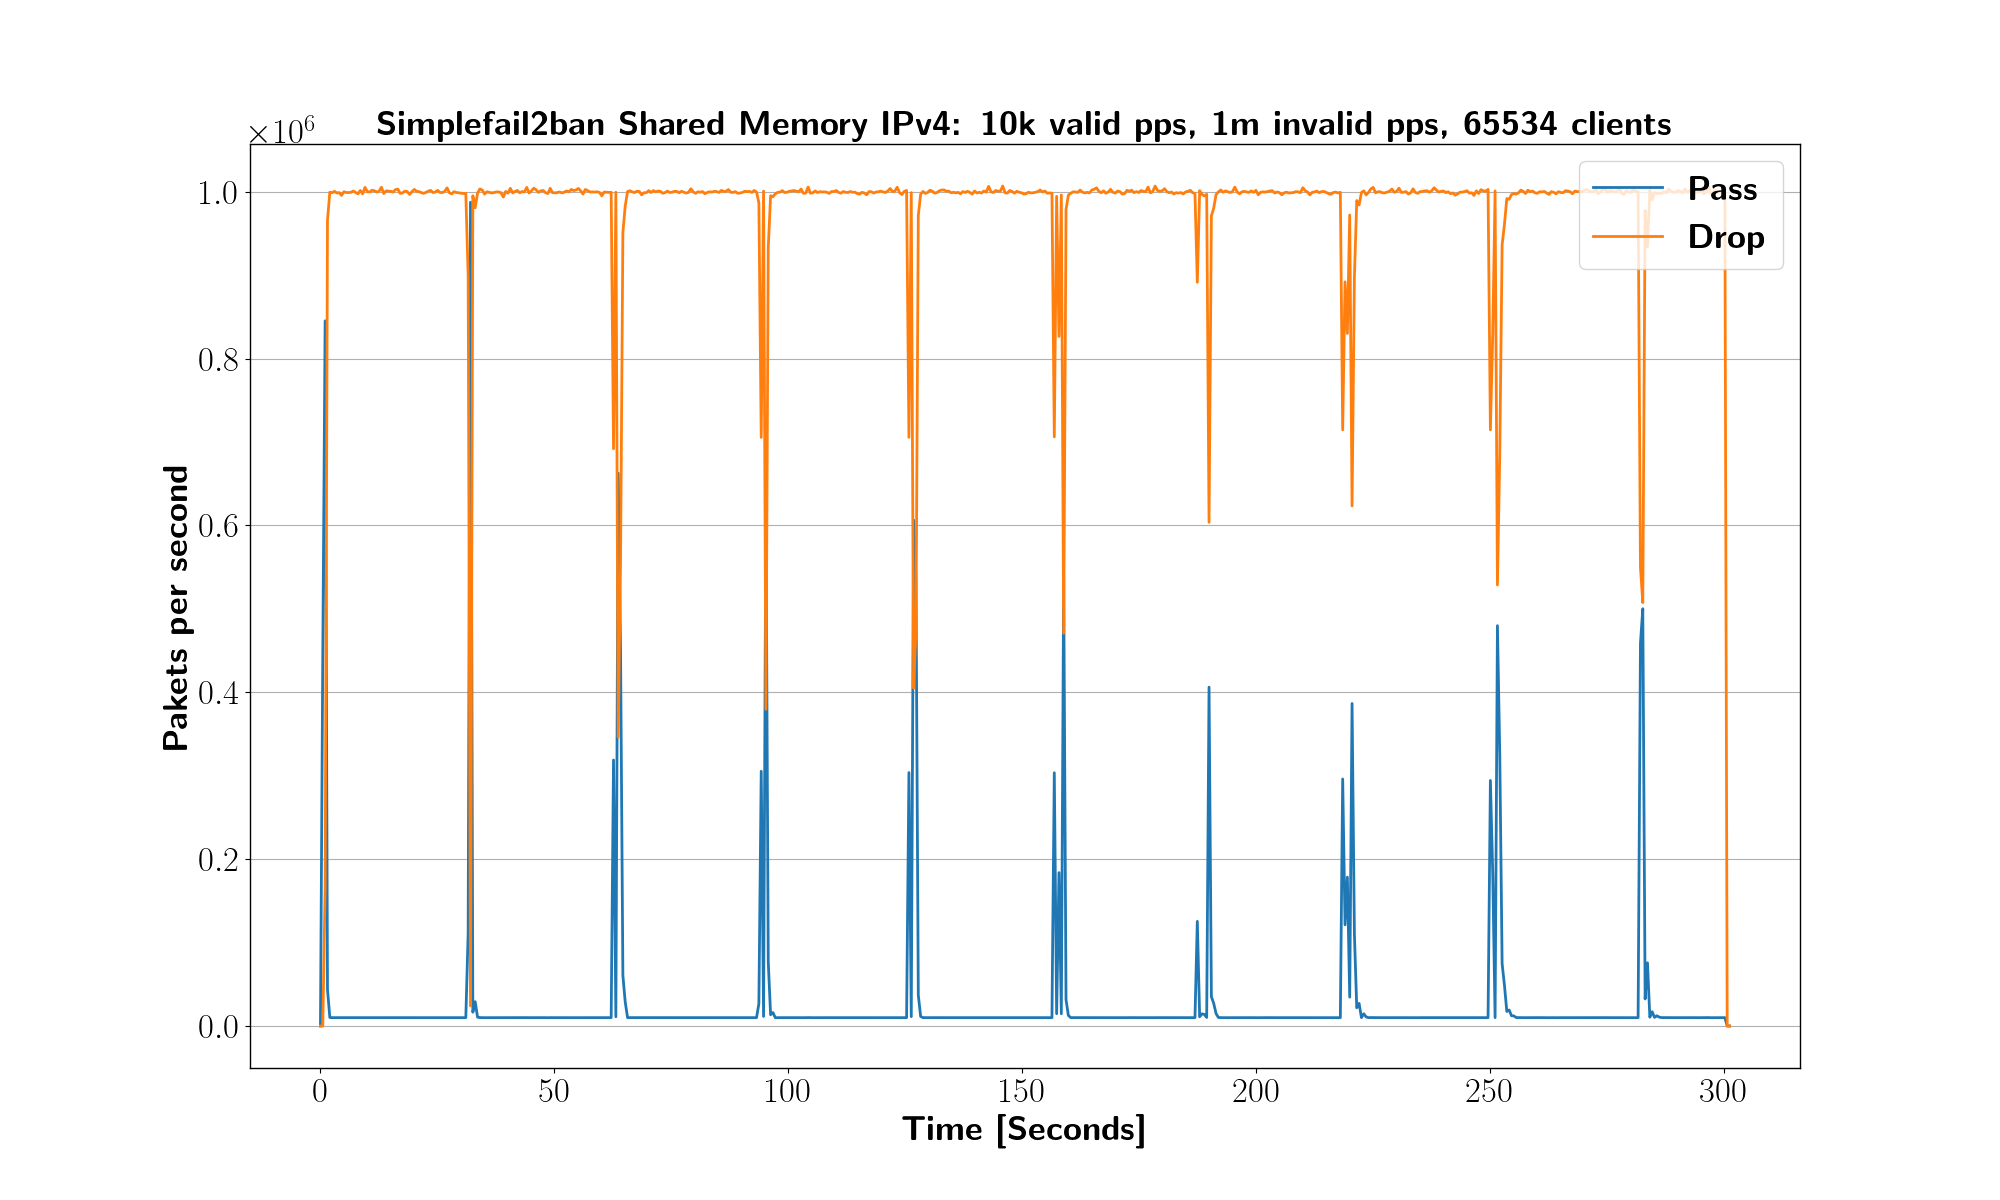
\includegraphics[width=1.2\textwidth]{images/simplefail2ban_shm_ipv4_v10k_iv1m_c65534.png}}
	\end{tabular}
	\begin{tabular}{lllll}
		\toprule
		\textbf{Total packets [$10^6$]} & \textbf{Packets dropped [$10^6$]} & \textbf{Relative drop [\%]} & \textbf{Log messages [$10^6$]} & \textbf{CPU [seconds]} \\ \midrule 
		303 & 294.34 & 98.88 & 4.61 & 15.52 \\
		\bottomrule
	\end{tabular}
	\caption[Simplefail2ban, Shared Memory, IPv4, 1m \ac{PPS}]{Simplefail2ban Shared Memory \ac{IPv4}, 10 thousand wanted \ac{PPS}, 10 million unwanted \ac{PPS}, 65534 clients.}
	\label{fig:simplefail2ban:shm:ip4:1m}
\end{figure}

\begin{figure}[!h]
	\centering
	\scriptsize
	\begin{tabular}{c}
    	\centerline{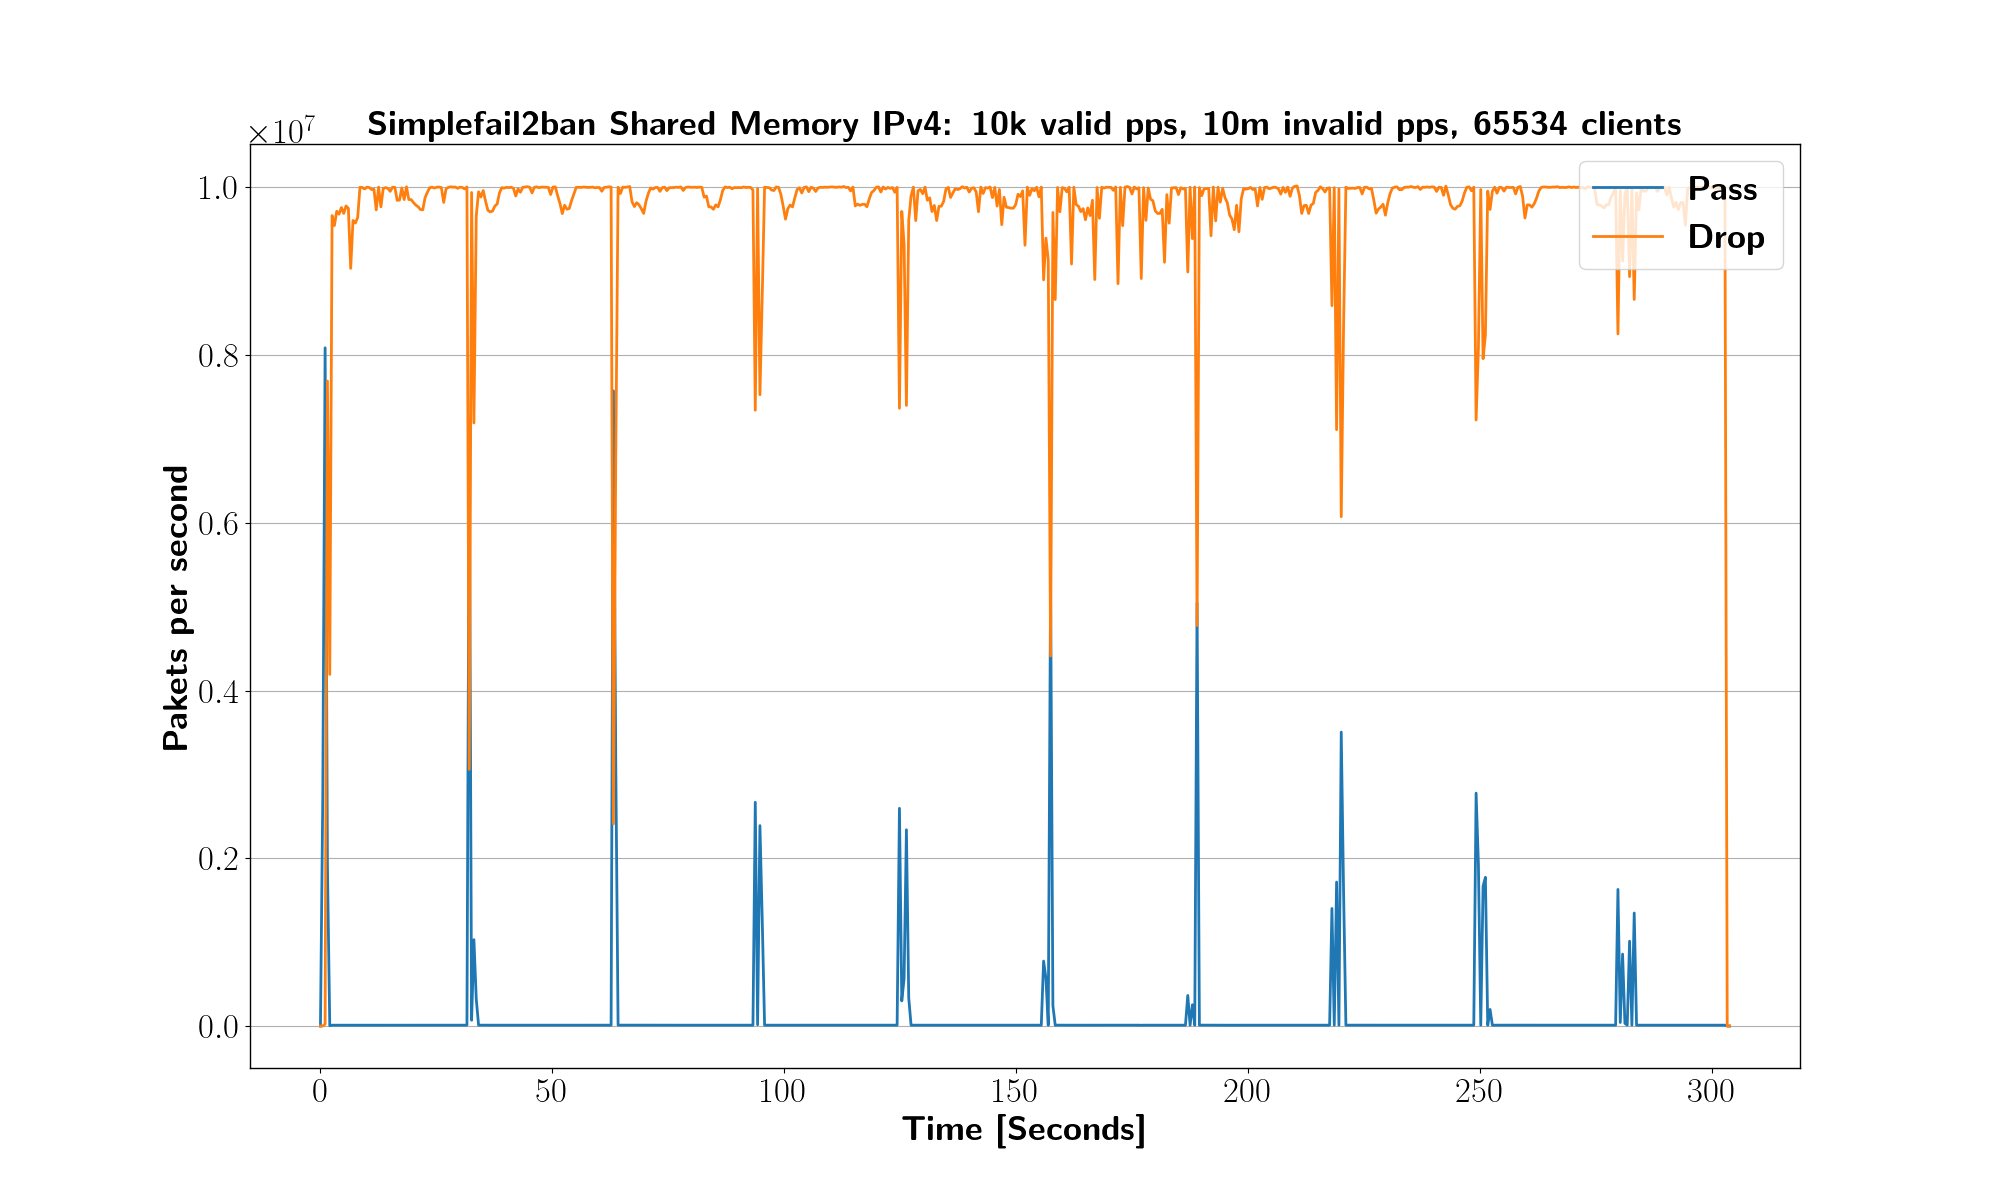
\includegraphics[width=1.2\textwidth]{images/simplefail2ban_shm_ipv4_v10k_iv10m_c65534.png}}
	\end{tabular}
	\begin{tabular}{lllll}
		\toprule
		\textbf{Total packets [$10^6$]} & \textbf{Packets dropped [$10^6$]} & \textbf{Relative drop [\%]} & \textbf{Log messages [$10^6$]} & \textbf{CPU [seconds]} \\ \midrule 
		2991.48 & 2948.51 & 96.72 & 7.69 & 25.59 \\
		\bottomrule
	\end{tabular}
	\caption[Simplefail2ban, Shared Memory, IPv4, 10m \ac{PPS}]{Simplefail2ban Shared Memory \ac{IPv4}, 10 thousand wanted \ac{PPS}, 10 million unwanted \ac{PPS}, 65534 clients.}
	\label{fig:simplefail2ban:shm:ip4:10m}
\end{figure}

\begin{figure}[!h]
	\centering
	\scriptsize
	\begin{tabular}{c}
    	\centerline{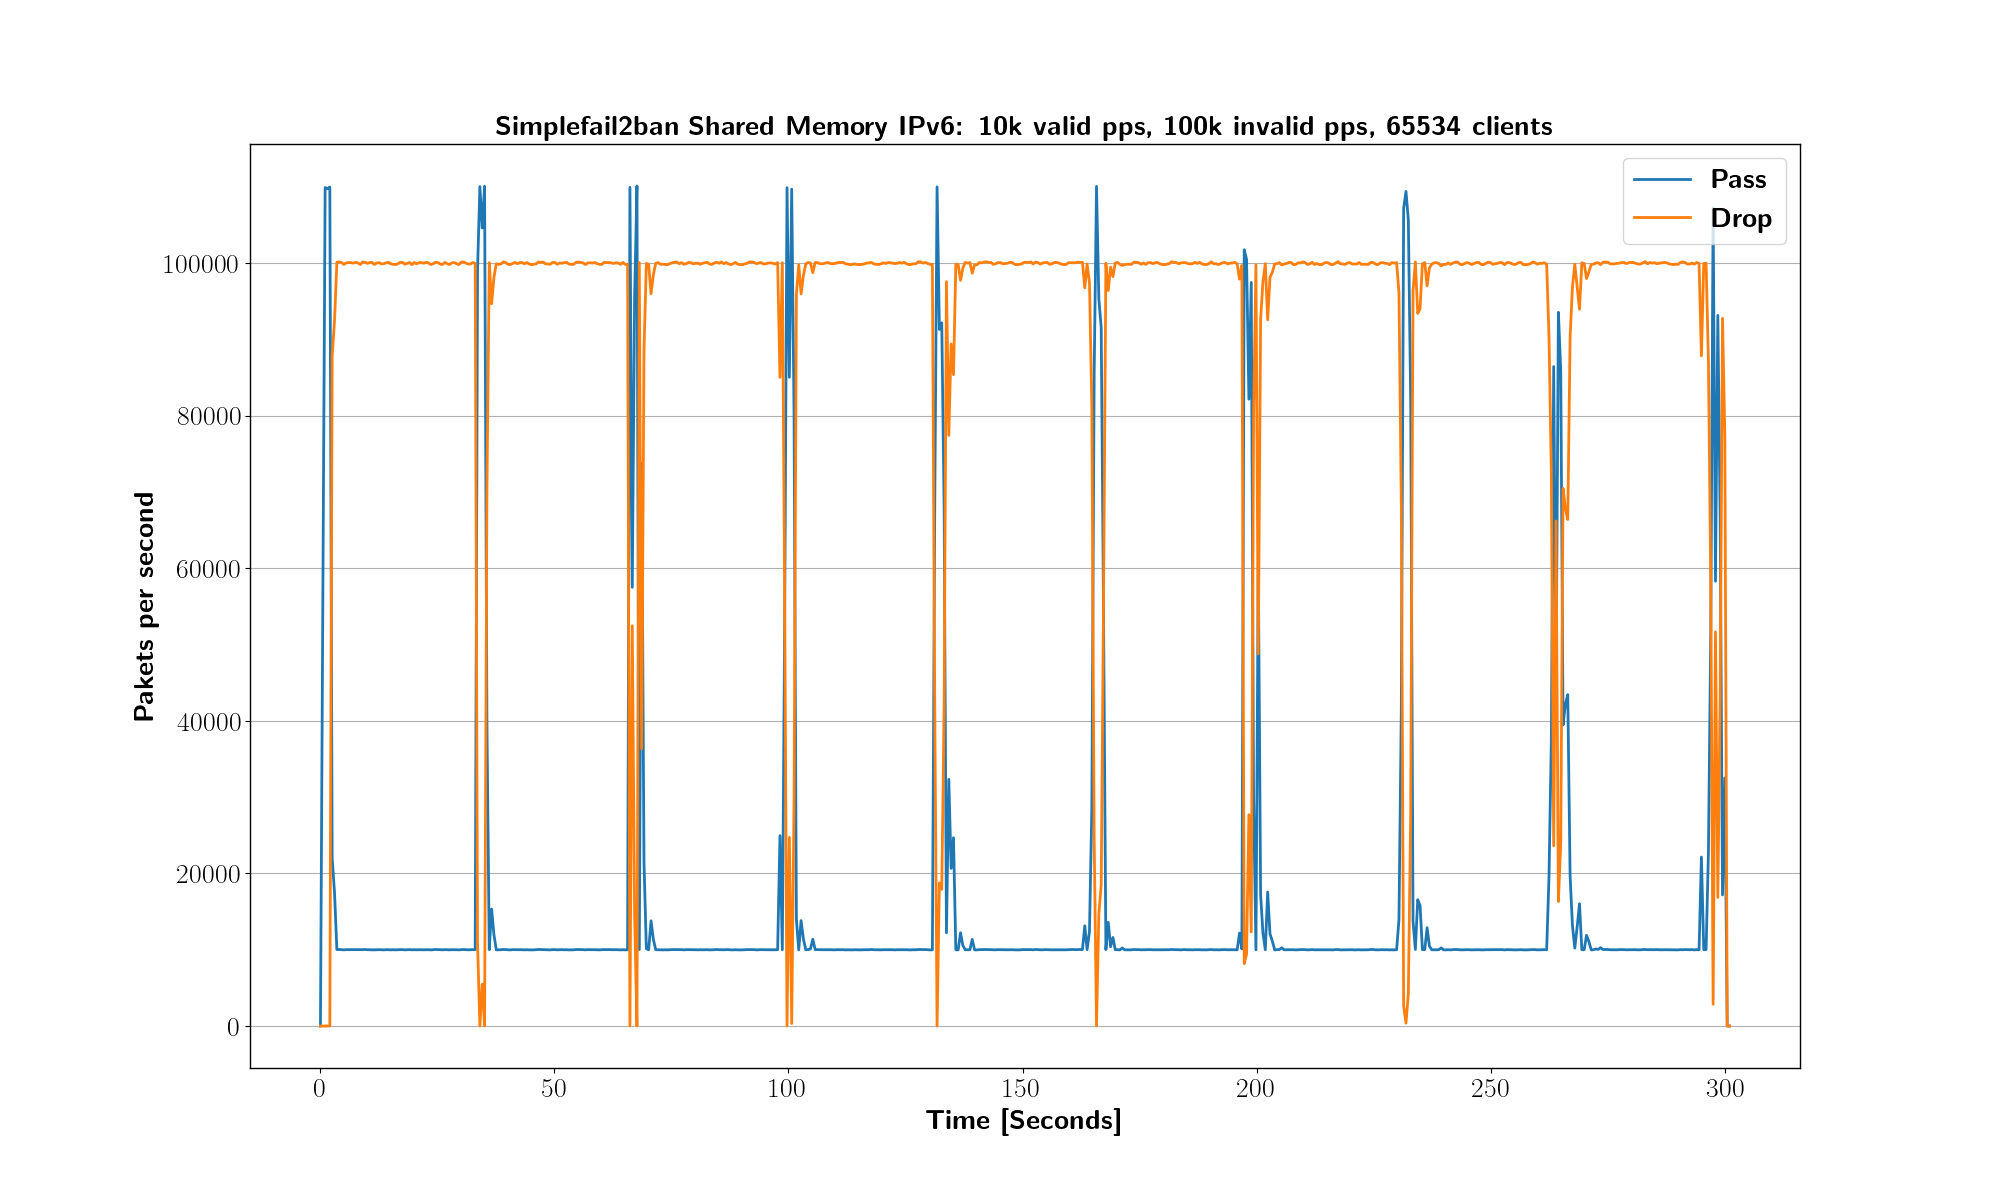
\includegraphics[width=1.2\textwidth]{images/simplefail2ban_shm_ipv6_v10k_iv100k_c65534.png}}
	\end{tabular}
	\begin{tabular}{lllll}
		\toprule
		\textbf{Total packets [$10^6$]} & \textbf{Packets dropped [$10^6$]} & \textbf{Relative drop [\%]} & \textbf{Log messages [$10^6$]} & \textbf{CPU [seconds]} \\ \midrule 
		33 & 27.95 & 99.67 & 2.05 & 15.55 \\
		\bottomrule
	\end{tabular}
	\caption[Simplefail2ban, Shared Memory, IPv6, 100k \ac{PPS}]{Simplefail2ban Shared Memory \ac{IPv6}, 10 thousand wanted \ac{PPS}, 100 thousand unwanted \ac{PPS}, 65534 clients.}
	\label{fig:simplefail2ban:shm:ip6:100k}
\end{figure}

\begin{figure}[!h]
	\centering
	\scriptsize
	\begin{tabular}{c}
    	\centerline{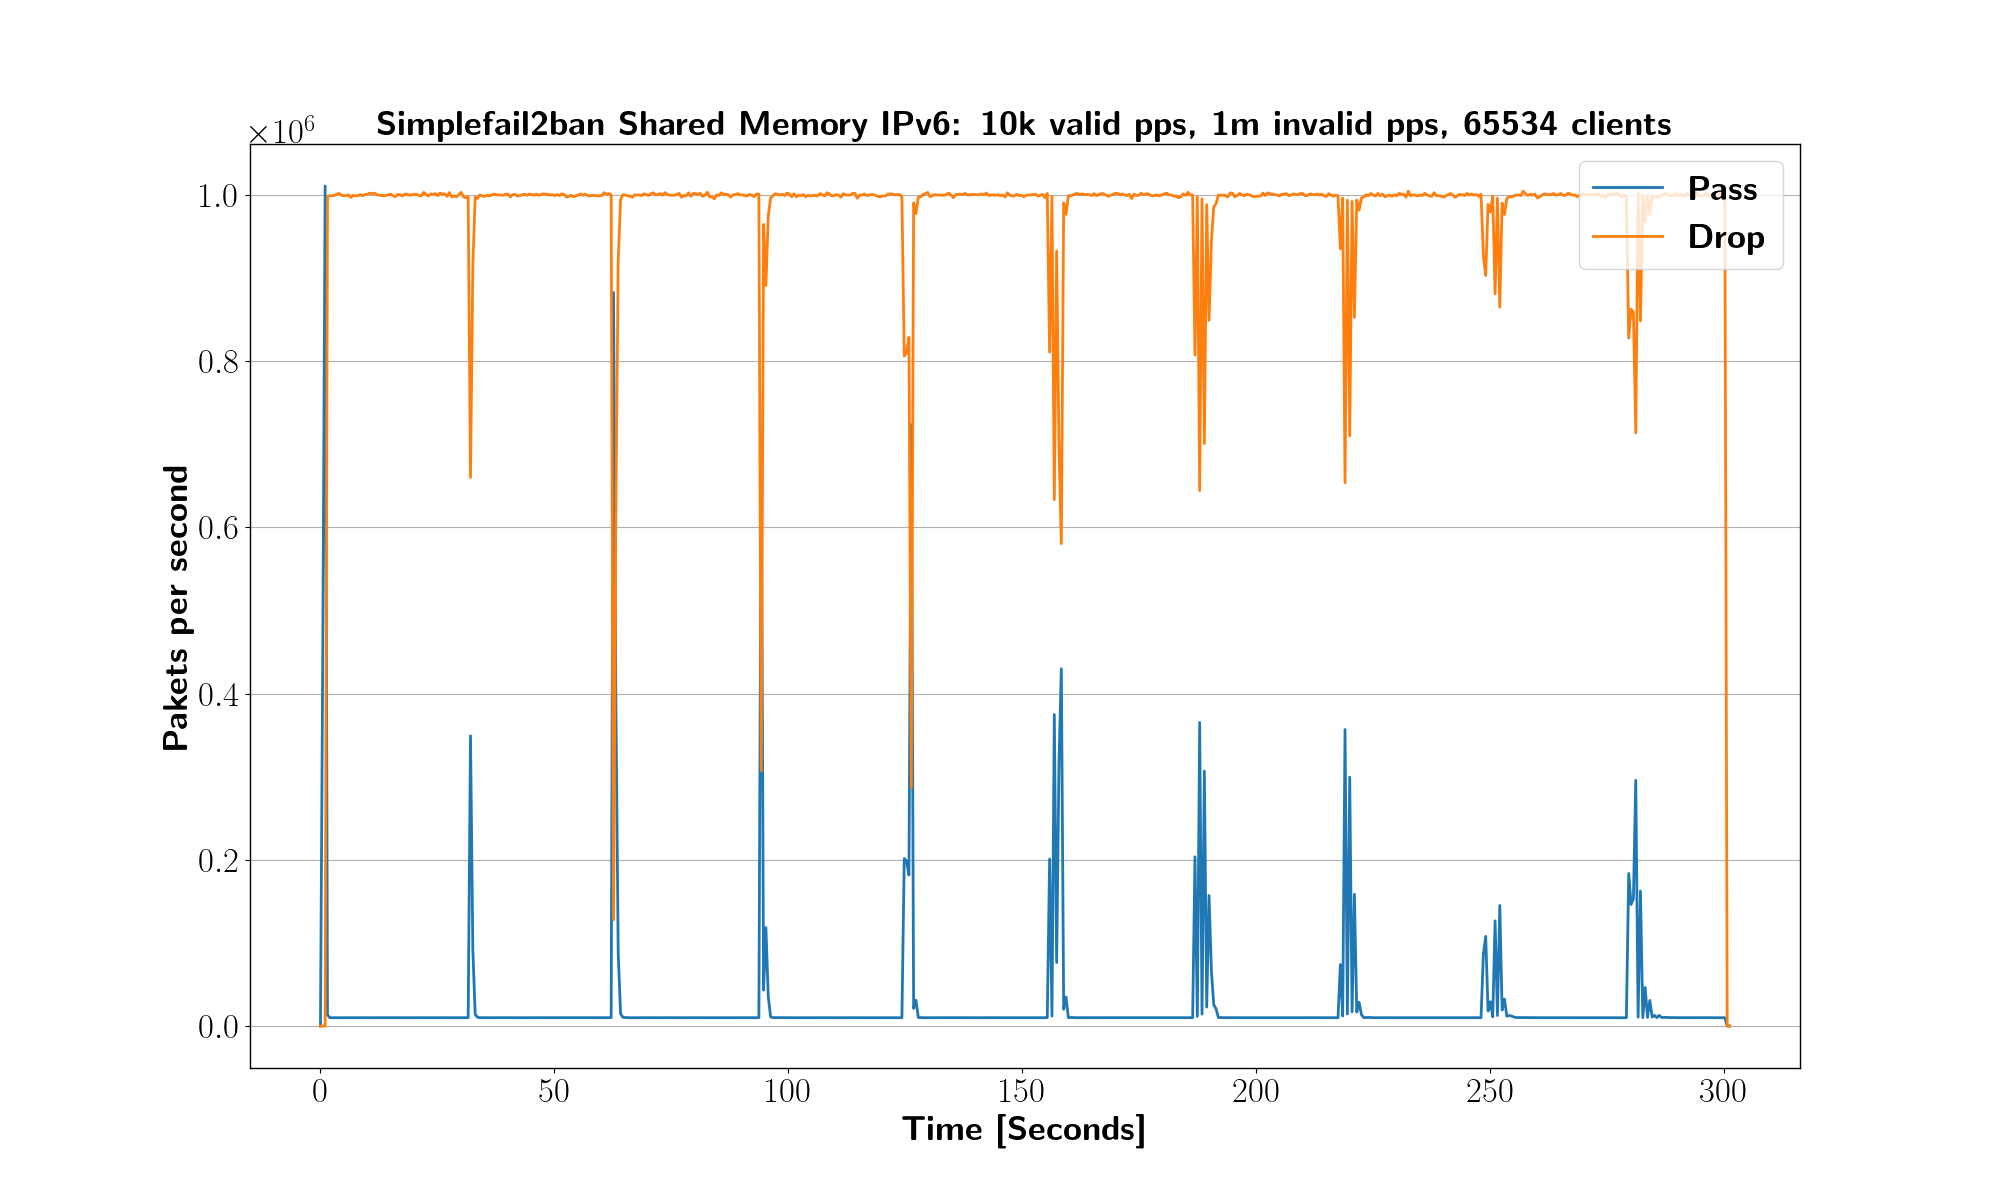
\includegraphics[width=1.2\textwidth]{images/simplefail2ban_shm_ipv6_v10k_iv1m_c65534.png}}
	\end{tabular}
	\begin{tabular}{lllll}
		\toprule
		\textbf{Total packets [$10^6$]} & \textbf{Packets dropped [$10^6$]} & \textbf{Relative drop [\%]} & \textbf{Log messages [$10^6$]} & \textbf{CPU [seconds]} \\ \midrule 
		303 & 294.77 & 98.9 & 4.39 & 17.46 \\
		\bottomrule
	\end{tabular}
	\caption[Simplefail2ban, Shared Memory, IPv6, 1m \ac{PPS}]{Simplefail2ban Shared Memory \ac{IPv6}, 10 thousand wanted \ac{PPS}, 1 million unwanted \ac{PPS}, 65534 clients.}
	\label{fig:simplefail2ban:shm:ip6:1m}
\end{figure}

\begin{figure}[!h]
	\centering
	\scriptsize
	\begin{tabular}{c}
    	\centerline{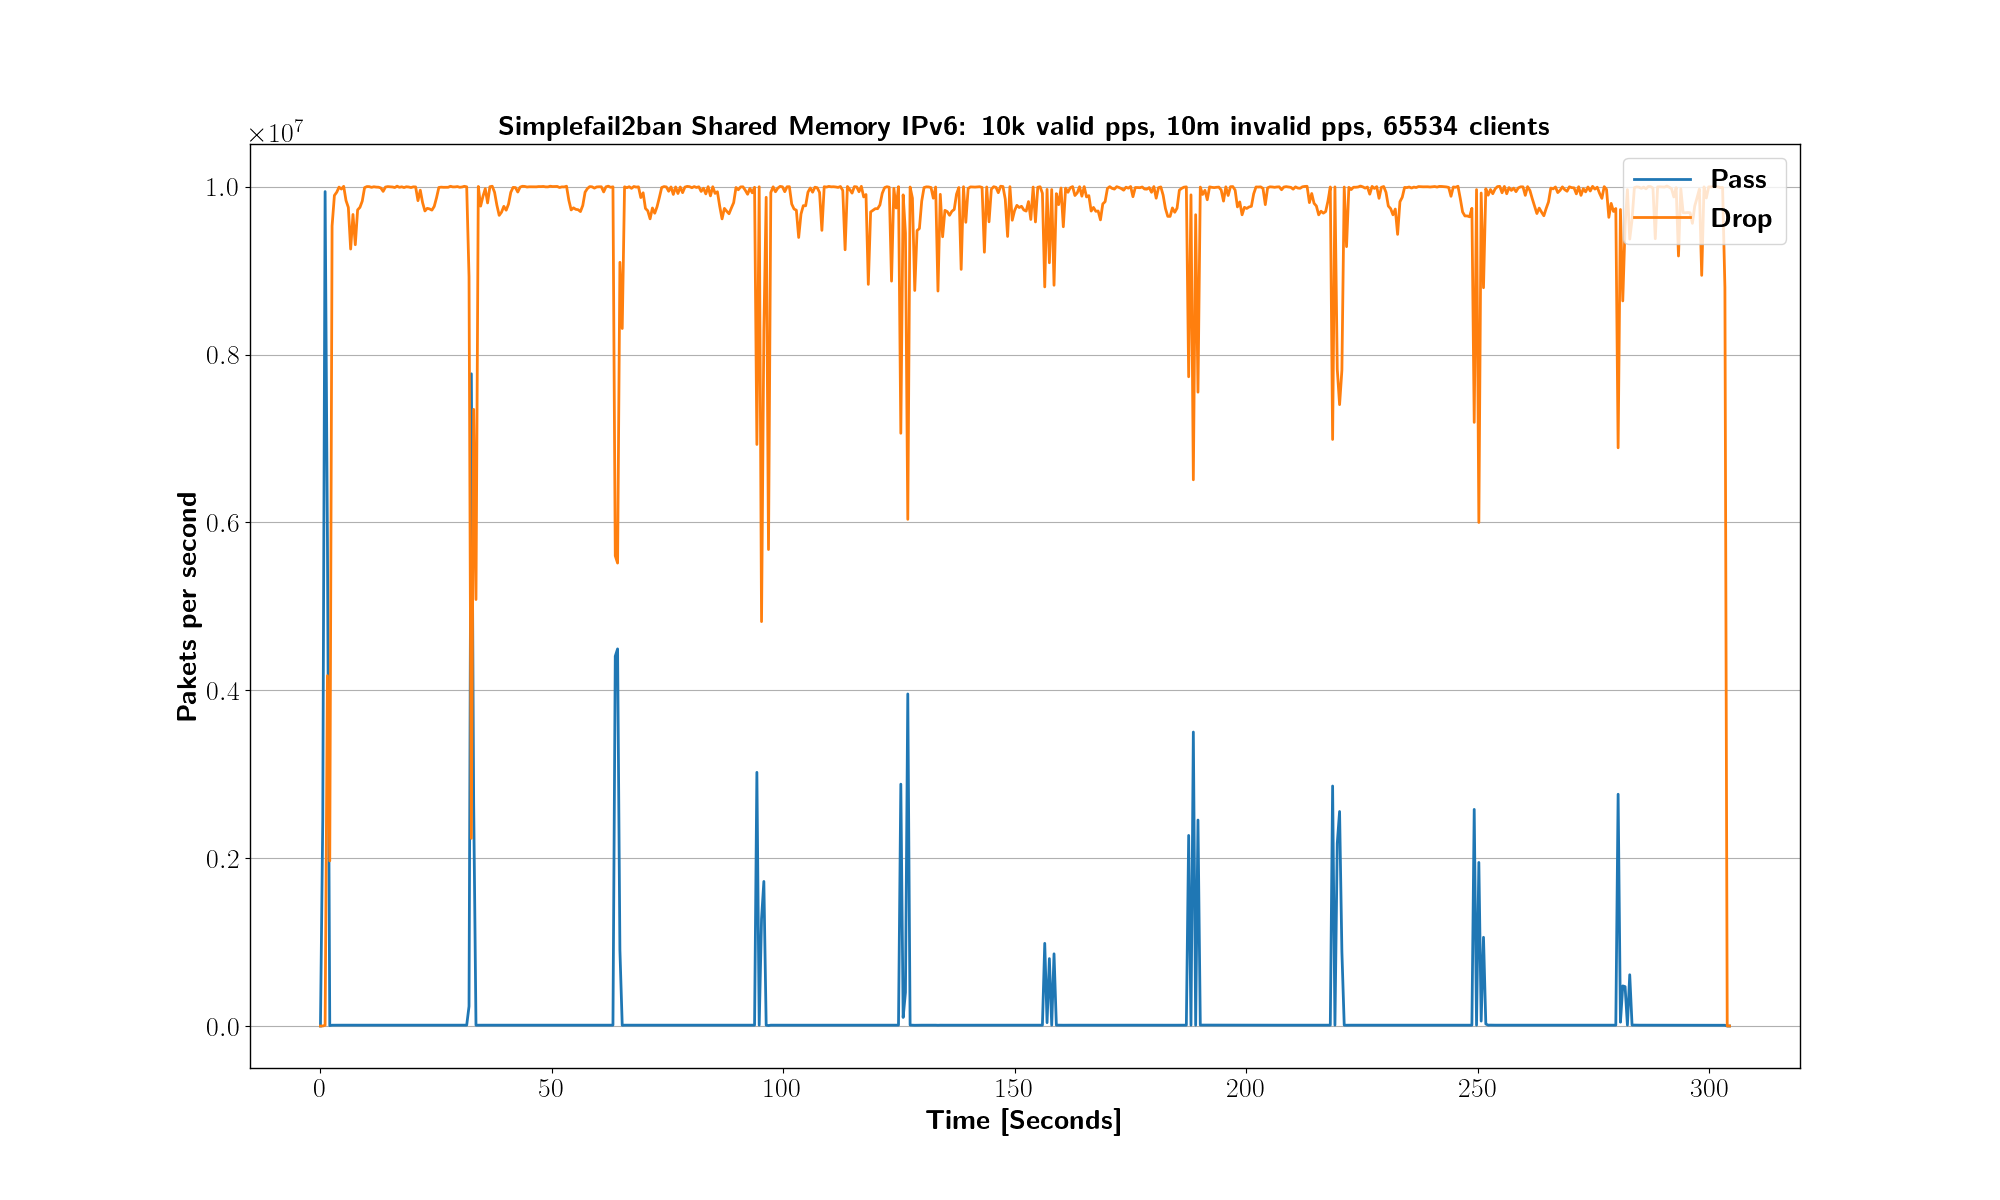
\includegraphics[width=1.2\textwidth]{images/simplefail2ban_shm_ipv6_v10k_iv10m_c65534.png}}
	\end{tabular}
	\begin{tabular}{lllll}
		\toprule
		\textbf{Total packets [$10^6$]} & \textbf{Packets dropped [$10^6$]} & \textbf{Relative drop [\%]} & \textbf{Log messages [$10^6$]} & \textbf{CPU [seconds]} \\ \midrule 
		2991.93 & 2947.1 & 98.66 & 8.88 & 32.36 \\
		\bottomrule
	\end{tabular}
	\caption[Simplefail2ban, Shared Memory, IPv6, 10m \ac{PPS}]{Simplefail2ban Shared Memory \ac{IPv6}, 10 thousand wanted \ac{PPS}, 10 million unwanted \ac{PPS}, 65534 clients.}
	\label{fig:simplefail2ban:shm:ip6:10m}
\end{figure}

%
% bibliography
%
\def\UrlBreaks{\do\/\do-}
% alphaurl is a special bibliography style which includes Hyperlinks 
% to papers
\begingroup
\sloppy
%\raggedright
\bibliographystyle{unsrt}
% bib file without extension
\bibliography{literature}
\endgroup


%\printindex 
 % Appendix etc.

\end{document}
